% Study guide for the team: everything in the evaluator report, explained twice (simple words, then technical words),
% with what to say, worked examples and likely questions. Build: report/guide/build.sh
\documentclass[11pt,a4paper,oneside]{report}
\usepackage[T1]{fontenc}
\usepackage[utf8]{inputenc}
\usepackage{mathptmx}
\usepackage[scaled=0.9]{helvet}
\usepackage{microtype}
\usepackage[a4paper,left=1.15in,right=1in,top=1in,bottom=1in]{geometry}
\usepackage{amsmath,amssymb}
\usepackage{graphicx,xcolor,booktabs,array,tabularx,longtable,enumitem,float}
\usepackage{fancyhdr,titlesec,setspace}
\usepackage[most]{tcolorbox}
\usepackage[hidelinks,bookmarksnumbered]{hyperref}
\usepackage{xurl}\urlstyle{tt}
\newcommand{\cpath}[1]{{\footnotesize\path{#1}}}
\graphicspath{{../figures/}{../diagrams/}}
\setstretch{1.12}\setlength{\parindent}{0pt}\setlength{\parskip}{6pt}
\setlist{itemsep=2pt,topsep=4pt,parsep=2pt}
\setcounter{tocdepth}{2}

\definecolor{simple}{HTML}{1B7F5C}
\definecolor{tech}{HTML}{2F5DA8}
\definecolor{say}{HTML}{B5651D}
\definecolor{warn}{HTML}{A33B3B}
\newtcolorbox{simplebox}{enhanced,breakable,colback=simple!6,colframe=simple,boxrule=0.7pt,arc=2pt,left=7pt,right=7pt,top=5pt,bottom=5pt,title={In simple words},fonttitle=\bfseries\sffamily\small,coltitle=white,colbacktitle=simple}
\newtcolorbox{techbox}{enhanced,breakable,colback=tech!5,colframe=tech,boxrule=0.7pt,arc=2pt,left=7pt,right=7pt,top=5pt,bottom=5pt,title={In technical words},fonttitle=\bfseries\sffamily\small,coltitle=white,colbacktitle=tech}
\newtcolorbox{saybox}{enhanced,breakable,colback=say!6,colframe=say,boxrule=0.7pt,arc=2pt,left=7pt,right=7pt,top=5pt,bottom=5pt,title={What to say},fonttitle=\bfseries\sffamily\small,coltitle=white,colbacktitle=say}
\newtcolorbox{warnbox}{enhanced,breakable,colback=warn!5,colframe=warn,boxrule=0.7pt,arc=2pt,left=7pt,right=7pt,top=5pt,bottom=5pt,title={Be careful here},fonttitle=\bfseries\sffamily\small,coltitle=white,colbacktitle=warn}
\newtcolorbox{examplebox}[1][]{enhanced,breakable,colback=gray!7,colframe=gray!60,boxrule=0.6pt,arc=2pt,left=7pt,right=7pt,top=5pt,bottom=5pt,title={#1},fonttitle=\bfseries\sffamily\small,coltitle=black,colbacktitle=gray!25}

\pagestyle{fancy}\fancyhf{}
\renewcommand{\headrulewidth}{0.4pt}
\fancyhead[L]{\small\itshape\nouppercase{\leftmark}}
\fancyhead[R]{\small Study guide: our project, explained}
\fancyfoot[C]{\small Page \thepage}
\fancypagestyle{plain}{\fancyhf{}\fancyfoot[C]{\small Page \thepage}}
\titleformat{\chapter}[display]{\bfseries\Large}{Part \thechapter}{6pt}{\Huge}
\titlespacing*{\chapter}{0pt}{-10pt}{16pt}
\titleformat{\section}{\bfseries\Large\color{tech}}{\thesection}{0.6em}{}
\titleformat{\subsection}{\bfseries\large}{\thesubsection}{0.6em}{}
\newcommand{\code}[1]{\texttt{\small #1}}
\newcommand{\cn}{C+N}
\newcommand{\q}[1]{\textbf{Q: #1}}
\renewcommand{\chaptermark}[1]{\markboth{#1}{}}

\begin{document}
\begin{titlepage}
\centering
{\Large\bfseries\color{tech} STUDY GUIDE}\\[10pt]
{\Huge\bfseries Probabilistic Cascading Failure and\\Agent-Assisted Root Cause Analysis\\for Microservice Systems}\\[14pt]
{\large What we built, why it works, what we measured, and what to say about it}\\[28pt]
\begin{tcolorbox}[colback=gray!6,colframe=gray!50,width=0.82\textwidth,boxrule=0.5pt]
\raggedright\small
This guide is for the four of us, not for the evaluator. The evaluator gets the \textbf{project report} (about 100 pages, formal). This guide is the long, plain version of the same project. Every topic appears three ways: \textbf{in simple words}, \textbf{in technical words}, and as \textbf{what to say} when someone asks. Read the simple box first. If you can explain that without looking, move to the technical one.
\end{tcolorbox}
\vfill
{\large Anish C \quad Royson Salis \quad Dhanush K Murthy \quad K Bharath Parmar}\\[4pt]
{\small Department of Artificial Intelligence \& Machine Learning, MITE Mangalore \quad 2026--2027}
\end{titlepage}
\tableofcontents
\chapter{How to use this guide}
\label{ch:howto}

\section{Two documents, two jobs}
We now have two documents about the same project, and they do different jobs.

\begin{itemize}
\item \textbf{The project report} (\code{report/main.pdf}, about 100 pages). This goes to the evaluator. It is formal, dense and complete. It has the equations, the tables, the screenshots, the references and the honest list of limits. People get tired of long reports, so we kept it close to 100 pages and cut everything that was not needed to support a claim.
\item \textbf{This study guide} (\code{report/guide/main.pdf}). This is for us. It is long on purpose. Nothing in it is new science: every number comes from the report. What it adds is explanation. It tells you what each part \emph{means}, why we built it that way, what the number really says, and what to answer when someone pokes at it.
\end{itemize}

\begin{saybox}
If an evaluator asks something and you do not remember the answer, the answer is in Part~\ref{ch:qa} (questions and answers). If you do not understand the answer, go to the part that explains the topic. Every part has a green box (simple words) and a blue box (technical words). Learn the green box first. The blue box is what you say when they want depth.
\end{saybox}

\section{How every part is built}
Each part follows the same pattern, so you always know where to look.

\begin{enumerate}
\item A green box: \textbf{in simple words}. A friend with no computer-science background should follow it.
\item A blue box: \textbf{in technical words}. The same idea with the proper terms, the numbers and the method.
\item Worked examples in grey boxes, with small numbers you can check by hand.
\item An orange box: \textbf{what to say}. Two or three sentences you can say out loud, in an order that works.
\item A red box when there is a trap: a claim that sounds stronger than the evidence, or a number that is easy to misquote.
\end{enumerate}

\section{The pitch at four lengths}
You need the same story at different lengths, depending on how much time the evaluator gives you. Practise all four.

\subsection{Thirty seconds}
\begin{saybox}
In a microservice system one failure spreads to the services that depend on it, so the operator gets a flood of alarms and cannot tell which service broke first. Our tool watches the containers from outside, over SSH, so we change nothing in the application. It builds the call graph, decides which services are behaving abnormally, ranks the likely root cause and predicts which services fall next. It needs no labelled data and no GPU.
\end{saybox}

\subsection{Two minutes}
\begin{saybox}
Add three things to the thirty-second version. First, \emph{how}: we read Docker state, statistics and each container's socket table, work out who calls whom from the listening port, and judge every service against its own recent normal. Second, \emph{what went wrong and how we fixed it}: our first machine-learning engine, a per-service Isolation Forest, flagged every service as 100\% anomalous the moment traffic stopped, because it could not tell ``everyone is quieter'' from ``one service is broken''. We replaced it with a load-aware model that first estimates how much the whole system's workload moved and then judges only what is left. On recordings with no faults and only changing load, the old engine was in alarm 23 to 52\% of the time and the new one 0\%. Third, \emph{how we know}: we injected 62 faults blind into two real systems we built, plus 84 live and 178 synthetic ones, and we report the results with confidence intervals, including the ones that were not significant.
\end{saybox}

\subsection{Five minutes}
Use the two-minute version, then add the cascade model (we learn, for each call edge, how often trouble crosses it, and use that to predict who falls next), the three engines you can switch between (Rules, ML, Hybrid) and the Detection engines page that shows all three side by side, and the honest limits (two real systems, no real users, brownouts of idle services are missed).

\subsection{Ten minutes, with the demo}
Run the demo in Part~\ref{ch:demo}: start the dashboard, show the 3D Islands view, break a container, show the incident page naming the root cause and the cascade, open the Detection engines page and show the three engines disagreeing in a useful way. Then finish on the results table.

\section{Where the ML depth is}
Part~\ref{ch:mlstory} tells the ML story. Parts~\ref{ch:deepforest} to~\ref{ch:deepeval} are the deep dives: the old model in detail (\ref{ch:deepforest}), the new model line by line with real worked output (\ref{ch:deepload}), the engine around it (\ref{ch:deepengine}) and every experiment behind each setting plus an ML question bank (\ref{ch:deepeval}). Read them in that order.

\section{The five numbers to remember}
If you remember nothing else, remember these. They are all in the report.

\begin{center}
\begin{tabular}{@{}rl@{}}
\toprule
\textbf{23--52\%} & time the old ML was in alarm when only the load moved (no fault)\\
\textbf{0\%} & the same for the new load-aware ML\\
\textbf{71\% vs 63\%} & faults caught \emph{and} correctly named, Hybrid vs Rules, on 62 real faults\\
\textbf{+8.1 points, $p=0.117$} & that difference, and it is \emph{not} statistically significant\\
\textbf{0.37 ms} & cost of one decision per service on one CPU core\\
\bottomrule
\end{tabular}
\end{center}

\begin{warnbox}
The 71\% against 63\% is the easiest number to overclaim. It is a real difference in our data, but with 62 faults it is not statistically significant. Say ``it points that way, and we say plainly that it is not significant''. Evaluators trust that sentence more than a bold claim. The \emph{strong} result is the 0\% against 23--52\%, which is large and clear.
\end{warnbox}

\chapter{The whole project as one story}
\label{ch:story}

Before any detail, learn the story. Every later part is one scene of it.

\section{Act one: a failure that spreads}
\begin{simplebox}
Think of a restaurant. The kitchen cannot get vegetables from the supplier, so the cooks slow down, so the waiters wait, so customers wait, so the manager gets angry calls from every table. If you only listen to the angry calls, the loudest one is a table, not the supplier. The real problem is two steps away from where the noise is.

Modern apps work like that restaurant. They are made of many small programs called \emph{services}. The checkout service calls the payment service, which calls the database. If the database gets slow, payment gets slow, then checkout gets slow, and the engineer on call sees alarms from all three. Which one is the cause? Usually not the loudest.
\end{simplebox}

\begin{techbox}
A microservice application is a set of independently deployed services connected by a directed call graph. A failure at a callee propagates \emph{against} the edges to the callers that wait on it. Under timeouts and retries the load amplifies, so within a minute many services alarm together (an \emph{alert storm}), and severity-based ranking points at a victim rather than the origin. Root-cause analysis (RCA) is the problem of identifying the originating service from the telemetry.
\end{techbox}

\section{Act two: the tools that exist, and why they did not fit us}
\begin{simplebox}
There are two families of tools. The first is clever research that uses neural networks to find the broken service. It needs lots of examples of past failures with the answer written next to them, it needs a graphics card, and it gives an answer you cannot check. The second family is the normal monitoring products. They are reliable, but they only start working after you change your application: add code, add helpers, add extra containers.

Small teams, and student projects like ours, often have neither the failure examples nor the permission to change the app. We wanted a tool that works from the \emph{outside}, learns what normal looks like by itself, and shows its working so a person can check it.
\end{simplebox}

\begin{techbox}
Recent localisation methods fuse metrics, traces and logs with graph neural networks or autoencoders (DiagFusion, DeepHunt, Eadro). They need labelled failures, GPU inference, and produce output an engineer cannot audit against the dashboard. Observability products (metrics scraping, distributed tracing, APM agents) need instrumentation in the application or a sidecar in every pod. Our setting is an unmodified Docker Compose stack reached over SSH, with no labels and one CPU core.
\end{techbox}

\section{Act three: what we built}
\begin{simplebox}
We built a program (the \emph{mapper}) that logs into the machine over SSH and looks at the containers from outside, the way a doctor looks at a patient: pulse (CPU), breathing (memory), who the patient is talking to (network connections). From the connections it draws a live map of which service calls which. For each service it learns what ``normal'' looks like, and raises a flag when the service moves away from normal. When flags appear, it works out which service most likely started it, and which healthy services are next in line.

It also has a 3D view, because a map of fifty services is easier to understand as a small city than as a tangle of lines.
\end{simplebox}

\begin{techbox}
The platform is about 36\,000 lines of TypeScript with 339 automated tests. A collector reads \code{docker ps/inspect/stats} and each container's \code{/proc/<pid>/net/tcp} over one SSH session. An evidence-weighted graph orients each edge by the listening port. A hybrid detector (load-aware residual model plus a robust rule layer, with container state as hard facts) raises the alarm. A ranker decomposes deviations and runs a personalised random walk. A cascade model with learned Beta--Binomial edge probabilities predicts who falls next. A dashboard shows everything in 2D and 3D, and a Detection engines page runs Rules, ML and Hybrid in parallel.
\end{techbox}

\section{Act four: the day our ML embarrassed us}
\begin{simplebox}
This is the most important scene, and the one an evaluator will remember if you tell it well.

Our first machine-learning engine learned, for each service, the pattern of its recent numbers. It worked fine on our fault experiments. Then, while testing the live tool, one of us stopped the traffic generator and switched to ML mode. \emph{Every service turned 100\% anomalous.} Nothing was broken. Traffic had simply stopped, so every number dropped, and the engine had never seen a quiet system and decided everything was wrong.

The lesson is simple to say: \textbf{the engine could not tell ``everybody got quieter'' from ``one service is sick''.} A real operator has this problem constantly, because traffic goes up and down all day.
\end{simplebox}

\begin{techbox}
The first engine kept two Isolation Forests per service, trained on a sliding window of its readings. A forest learns the shape of recent readings; a change of workload falls outside that shape for \emph{all} services at once. On our fault-free workload recordings it was in alarm 23\% (organic traffic on/off) and 52\% (closed-loop load stepped $2,8,2,0,20,2$ visitors) of the time. The other detectors we tried (k-NN, Mahalanobis, HBOS, the ensemble) did the same or worse, because they all model the readings themselves. The failure was hidden in our benchmarks by a replay bug (Part~\ref{ch:mlstory}) that deleted idle stretches from the recordings.
\end{techbox}

\section{Act five: the fix}
\begin{simplebox}
The fix is an idea, not a bigger model. Before judging any single service, ask: \emph{how much did the whole system's workload change in this moment?} If every busy service got twice as busy, that is a traffic change, and it is not a fault. Remove that shared change, and then judge each service on what is left. A real fault shows up in one service (or a few); a traffic change shows up in all of them by about the same amount. A median over many services is hard to move with one broken service, so it measures the shared part cleanly.

On the same fault-free recordings the new engine was in alarm 0\% of the time, and on the injected faults it caught about as many as the old one.
\end{simplebox}

\begin{techbox}
The load-aware residual model computes a load factor $L(t)$, the median log-shift of the signals that carry traffic (network in/out, request rate, CPU) over all busy services, then judges each service's signals against what $L(t)$ predicts: a robust $z$ under two hypotheses, ``ignores load'' ($b=0$) and ``follows load'' ($b=b_f$, a ridge-estimated slope), taking the smaller $z$. The spread is the larger of the MAD and the distance to the 90th percentile in the direction that matters. Only readings under the alarm line enter the training window, so a fault never becomes the baseline. Result: 0\% time in alarm on both workload recordings, with the same accuracy on injected faults (71\% against 69\% caught and named on the real faults).
\end{techbox}

\section{Act six: how we know any of it is true}
\begin{simplebox}
Anyone can say a tool works. We tried to prove it fairly. We built two realistic applications ourselves (an online shop and a bank), put them on cloud machines, and used a separate \emph{fault injector} that breaks containers at random times without telling the mapper. The injector writes the true answers in a private notebook that nobody reads until the end. Then we compare the mapper's answers with the notebook. We also ran 84 more faults live, 178 faults on simulated systems the tool had never seen, and fault-free recordings to count false alarms. We report the results with error bars, and we write down the things that did not work.
\end{simplebox}

\begin{saybox}
End your story with the honesty point. ``We report what did not work: the random walk is not statistically better than ranking by anomaly alone on these benchmarks, learned directions do not beat the name rule when names exist, and our own measurement had two bugs that made the engines look better than they were. We fixed both.'' That makes everything else you said more believable.
\end{saybox}

\chapter{The problem, stated four ways}
\label{ch:problem}

\section{Why this problem is hard}
\begin{simplebox}
Four things make it hard, and each one is a reason a piece of our system exists.

\begin{enumerate}
\item \textbf{Nobody knows who calls whom.} The documentation says one thing, the running system does another. If you do not know the map, you cannot follow a failure along it. \emph{Our answer: read the real connections from each container.}
\item \textbf{The loudest alarm is usually a victim.} Ranking by how bad a number looks points at the wrong service. \emph{Our answer: ask how much of a service's trouble is explained by the services it depends on.}
\item \textbf{Nobody sees what is coming.} Operators find out a service is hurt only when it alarms. \emph{Our answer: learn how often trouble crosses each connection and warn about the next services.}
\item \textbf{Black boxes are hard to trust at 3 a.m.} \emph{Our answer: every score is plain arithmetic and every part is shown on screen.}
\end{enumerate}
\end{simplebox}

\begin{techbox}
Formally: a system is a set $S$ of $N$ services with a directed call graph; an edge $u\to v$ means $u$ calls $v$. Every $\Delta=5$\,s the collector yields, for each service $s$, a reading $x_s(t)\in(\mathbb R\cup\{\varnothing\})^8$: CPU, memory, CPU throttling, network in and out, request rate, error share and 95th-percentile latency. $\varnothing$ marks a metric that was not reported and is \emph{never} replaced by zero, because a stopped container must be distinguishable from an idle one. Each reading comes with a container state (running, paused, restarting, exited, detached). At time $t$, using only readings up to $t$, the pipeline must decide (i) whether an incident is in progress, (ii) which service $r$ is its root cause, (iii) which healthy services will be affected before it ends, and (iv) what kind of fault it is --- without labelled failures, without changing any application, and well inside the 5\,s collection period.
\end{techbox}

\section{The four linked sub-problems and where we solve each}
\begin{center}
\small
\begin{tabularx}{\textwidth}{>{\raggedright\arraybackslash}p{3.3cm}>{\raggedright\arraybackslash}X>{\raggedright\arraybackslash}p{4cm}}
\toprule
\textbf{Sub-problem} & \textbf{What it means} & \textbf{Where in this guide}\\
\midrule
Invisible dependencies & Recover the call graph and its direction without instrumentation & Parts~\ref{ch:observe} and~\ref{ch:graph}\\
Alert storms & Decide who is abnormal, then who is the \emph{origin} among them & Parts~\ref{ch:detect}, \ref{ch:mlstory}, \ref{ch:rank}\\
No view of the future & Predict the next affected services; warn early & Parts~\ref{ch:cascade}, \ref{ch:more}\\
Black-box output & Show evidence for every number, in the UI and in the tests & Parts~\ref{ch:ui}, \ref{ch:system}\\
\bottomrule
\end{tabularx}
\end{center}

\section{What the project is \emph{not}}
This matters in a viva, because evaluators like to test the edges of a claim.

\begin{itemize}
\item It is \textbf{not distributed tracing}. There are no request IDs and no spans. The ``Traces'' page shows sampled TCP connection snapshots, not requests. If someone asks ``can you follow one request across services?'', the honest answer is no.
\item It does \textbf{not read application payloads} and does \textbf{not need code changes}.
\item It does \textbf{not use a language model}. The ``assistant'' is a transparent composition of statistical models. A language-model agent on top of the structured evidence is listed as future work.
\item It was \textbf{not tested on Kubernetes}. It targets Docker hosts reached over SSH.
\item It is \textbf{not a replacement for an APM suite}. It is a first-line triage tool.
\end{itemize}

\begin{saybox}
When asked ``is this AI?'': ``Yes, in the sense that it learns what normal looks like from data without labels, using robust statistics and a probabilistic cascade model. No, in the sense of a neural network or an LLM. We chose that on purpose, because the people who need it cannot supply labels or GPUs, and cannot audit a black box.''
\end{saybox}

\section{What ``agent-assisted'' means in the title}
\begin{simplebox}
The title says ``agent-assisted''. In our project there are two helpers. The \emph{collector agent} is the part that goes and looks at the machine. The \emph{diagnosis assistant} is the part that thinks about what it saw and tells the engineer: here is the likely cause, here is who is next, here is the type of fault, here is what to check. Neither one changes the application. Neither one uses a chat model.
\end{simplebox}

\begin{techbox}
We describe the two agents with the PEAS scheme. \textbf{Collector agent:} performance = complete, timely, truthful readings with correct edges and directions; environment = a Docker host over SSH running an unknown stack; actuators = SSH commands from a fixed catalogue; sensors = Docker state and statistics, socket tables, logs, interface counters. \textbf{Diagnosis assistant:} performance = caught-and-named rate, alarm time and prediction calibration; environment = the evidence-weighted graph and the readings it holds; actuators = incidents, rankings, predictions, runbooks and explanations in the dashboard; sensors = readings, container facts, graph and learned directions.
\end{techbox}

\begin{warnbox}
Do not say ``autonomous agent'' or ``agentic AI''. The only action the mapper takes on a host is restarting a container that exited with a non-zero code, a few times at most, and that can be switched off. Everything else is observation and advice.
\end{warnbox}

\chapter{The maths primer: every tool we use, from scratch}
\label{ch:primer}

You do not need to be a statistician to explain this project. You need to understand about ten small ideas. Each one below has a plain explanation, the formula, and a worked example with small numbers you can check on paper.

\section{Median and why we prefer it to the average}
\begin{simplebox}
The average adds everything up and divides. The median lines everything up and takes the middle one. Imagine five services using CPU of 10, 11, 10, 12 and 95 per cent. The average is 27.6, which describes nobody. The median is 11, which describes the typical service. One crazy value drags the average and hardly touches the median. Because we are trying to \emph{detect} crazy values, we must not let them pollute the measure of normal. So we use the median.
\end{simplebox}
\begin{examplebox}[Check it]
Values: $10,\ 11,\ 10,\ 12,\ 95$. Sorted: $10,10,11,12,95$. Middle (3rd) value: $11$. Average: $(10+11+10+12+95)/5=138/5=27.6$.
\end{examplebox}

\section{MAD: how spread out is ``normal''?}
\begin{simplebox}
To say a number is ``far from normal'' we need a ruler for how far is far. The ruler is the typical distance of values from the median. We take the distance of each value from the median, then take the median of those distances. That is the MAD (median absolute deviation). It ignores crazy values for the same reason the median does.
\end{simplebox}
\begin{examplebox}[Check it]
Values $10,10,11,12,95$, median $11$. Distances from the median: $1,1,0,1,84$. Sorted: $0,1,1,1,84$. Median distance: $1$. So MAD $=1$. A standard deviation would be about 37, ruined by the 95. Multiplying MAD by $1.4826$ makes it comparable to a standard deviation for bell-shaped data, so the robust $z$-score is $(x-11)/(1.4826\times1)$. For $x=95$: $z=84/1.4826\approx56.7$, hugely abnormal. For $x=12$: $z\approx0.67$, normal.
\end{examplebox}

\section{The robust $z$-score and ``one-sided''}
\begin{simplebox}
A $z$-score says how many rulers away from normal a value is. We only care about the \emph{bad} direction for most signals. CPU going \emph{down} is not a problem; it goes down after every restart. CPU going up is. So for CPU, memory, throttling, errors and latency we count only increases (``one-sided''). For traffic we count both directions, because traffic collapsing to zero is also a sign of trouble.
\end{simplebox}

\section{Log scale: ``twice as much'' means the same thing everywhere}
\begin{simplebox}
Think of the difference between 10 and 20 requests, and between 10\,000 and 20\,000. Both are ``twice as busy''. On a normal scale the second is a bigger jump. On a log scale both are the same step (about 0.69). We use the log scale so a doubling means the same thing to every service. We add a small ``unit'' inside the log so that tiny flickers on idle services do not look like big events.
\end{simplebox}
\begin{examplebox}[Check it]
$\ln 20-\ln 10=\ln 2\approx0.693$ and $\ln 20\,000-\ln 10\,000=\ln 2\approx0.693$. With a unit $u=0.1$ for requests: $x=\ln(v+0.1)$. For $v=0$: $x=\ln 0.1=-2.30$; for $v=0.1$: $x=\ln 0.2=-1.61$. A tiny flicker of $0.1$ requests per second moves the value by $0.69$, but the floor on the spread (0.3) keeps that from becoming an alarm.
\end{examplebox}

\section{Percentiles and the tail-aware spread}
\begin{simplebox}
The 90th percentile is the value that 90\% of readings are below. If a signal is quiet most of the time but jumps every few minutes, its median and MAD are tiny, so the ordinary jumps look like emergencies. We therefore make the ruler at least as long as the distance from the median to the 90th percentile. Jumps that happen regularly are then part of normal.
\end{simplebox}
\begin{examplebox}[Check it]
A bursty signal with 100 readings: 90 are around $1.0$ (MAD 0.05) and 10 are around $3.0$. The median is $1.0$, the MAD-based spread is $0.074$, so a reading of $3.0$ gives $z\approx27$: a false alarm on an ordinary burst. The 90th percentile is about $3.0$ (the lower end of the jumps), so the tail spread is $(3.0-1.0)/1.2816\approx1.56$. Now $3.0$ gives $z\approx1.3$: normal.
\end{examplebox}

\section{Regression and the ridge idea}
\begin{simplebox}
Regression draws the best straight line through a cloud of points. Here the points are: on the horizontal axis, how much the whole system's load moved; on the vertical axis, how much one particular signal moved. The slope of the line says how strongly that signal follows the load: slope 1 means it moves one for one; slope 0 means it ignores the load. Ridge adds a gentle pull toward a sensible starting slope, so when we have almost no data the slope does not swing wildly.
\end{simplebox}
\begin{examplebox}[Check it]
Slope formula with a prior: $b=\dfrac{\sum dL+\kappa b^0}{\sum L^2+\kappa}$. Suppose there are only three points: $L=(0.1,\,0.2,\,0.1)$ and $d=(0.1,\,0.25,\,0.12)$. Then $\sum dL=0.01+0.05+0.012=0.072$ and $\sum L^2=0.01+0.04+0.01=0.06$. With no prior the slope is $0.072/0.06=1.2$. With $\kappa=60$ and a prior slope $b^0=1$: $b=(0.072+60)/(0.06+60)=60.072/60.06\approx1.0002$. The data are too thin to move the slope, so it stays at the prior. After a big load swing, $\sum L^2$ becomes large and the data start to dominate.
\end{examplebox}

\section{Beta--Binomial: learning a probability from experience}
\begin{simplebox}
You want the chance that trouble crosses a link. Start with a mild guess (50\%), worth the evidence of two imaginary trials. Each time trouble reaches the caller, that is a success; each time it does not, a failure. The estimate is $(\text{successes}+1)/(\text{trials}+2)$ with our prior. More trials, and the estimate trusts the data more than the guess. (Part~\ref{ch:cascade} has a table of this.)
\end{simplebox}

\section{Noisy-OR: combining routes}
\begin{simplebox}
If there are two independent ways something can happen, the chance that it happens is: one minus the chance that \emph{neither} way works. If route A works 80\% of the time, route B works 40\% of the time, then neither works with probability $0.2\times0.6=0.12$, so at least one works with probability $0.88$.
\end{simplebox}

\section{PageRank and the random walk}
\begin{simplebox}
Picture a person wandering a city, choosing the next street at random but preferring busy streets. After wandering for a very long time, count the fraction of time spent in each neighbourhood. The neighbourhoods with the highest fraction are the most ``central'' to the walk. In our case, the walker prefers to move toward abnormal services and to stay on a service whose trouble nothing downstream explains. The service with the highest fraction is the best candidate for the origin. The ``restart'' means that with probability 0.15 the walker teleports back to an abnormal service, which stops it from wandering off to irrelevant parts of the map.
\end{simplebox}

\section{ROC, AUROC and average precision}
\begin{simplebox}
Suppose a detector gives every service-moment a score, and some of those moments really had a fault. Sort by score. A good detector has the faulted moments near the top. \textbf{AUROC} is the chance that a randomly chosen faulted moment scores higher than a randomly chosen healthy one: 1.0 is perfect, 0.5 is guessing. \textbf{Average precision} cares about how clean the top of the list is: if the top ten scores are all real faults, AP is high.
\end{simplebox}

\section{Confidence intervals and the bootstrap}
\begin{simplebox}
Any rate measured on a small number of faults wobbles. The bootstrap estimates the wobble by re-running the experiment many times on re-shuffled versions of the same data (picking faults with replacement) and looking at the spread of results. The middle 95\% of those results is the 95\% confidence interval. A comparison between two engines is trustworthy only when the interval for the \emph{difference} does not include zero.
\end{simplebox}

\section{Calibration}
\begin{simplebox}
A prediction is calibrated if it keeps its promises. If a forecaster says ``70\% chance'' on a hundred days, it should have rained on about seventy. We group predictions into bins by predicted probability and compare the average predicted probability with the actual fraction that came true in each bin. The expected calibration error (ECE) is the weighted average gap. Smaller is better.
\end{simplebox}

\chapter{How the system works, end to end}
\label{ch:system}

\section{One five-second heartbeat}
\begin{simplebox}
The mapper has a heartbeat. Every five seconds it does the same loop, over and over, for as long as it runs:

\begin{enumerate}
\item \textbf{Look.} Ask each machine what containers are running and how busy each one is.
\item \textbf{Listen.} Ask each container who it is currently talking to.
\item \textbf{Update the map.} Add new connections, drop old ones, work out who is the caller on each.
\item \textbf{Judge.} For every service, ask: is this normal for \emph{you}, given how busy the system is?
\item \textbf{Decide.} If something looks wrong, open an incident and work out the likely origin.
\item \textbf{Predict.} Work out which healthy services are likely to be hurt next.
\item \textbf{Show.} Push all of it to the dashboard.
\end{enumerate}

The whole thing takes a few milliseconds of computing. The rest of the five seconds is waiting.
\end{simplebox}

\begin{techbox}
One cycle: (1) collector polls \code{docker ps}, \code{inspect}, \code{stats} and reads \code{/proc/<pid>/net/tcp} and \code{/proc/<pid>/net/dev} per container; (2) \code{GraphStore} merges declared edges (from the Compose file) with observed ones, orients each socket by listening port and expires an observed edge ten minutes after its last sighting; (3) the three engines run in parallel on the same readings (rules score; ML engine with load factor, residual levels, walk, forecast, cascade; fused Hybrid); (4) \code{IncidentManager} builds the evidence for the \emph{active} engine only, calls the root-cause engine and opens, updates or resolves the incident; (5) the server pushes a \code{graph-update} over the WebSocket, coalesced to at most one frame per three seconds. The decision window costs about 0.37\,ms per service on one core.
\end{techbox}

\begin{figure}[H]
\centering
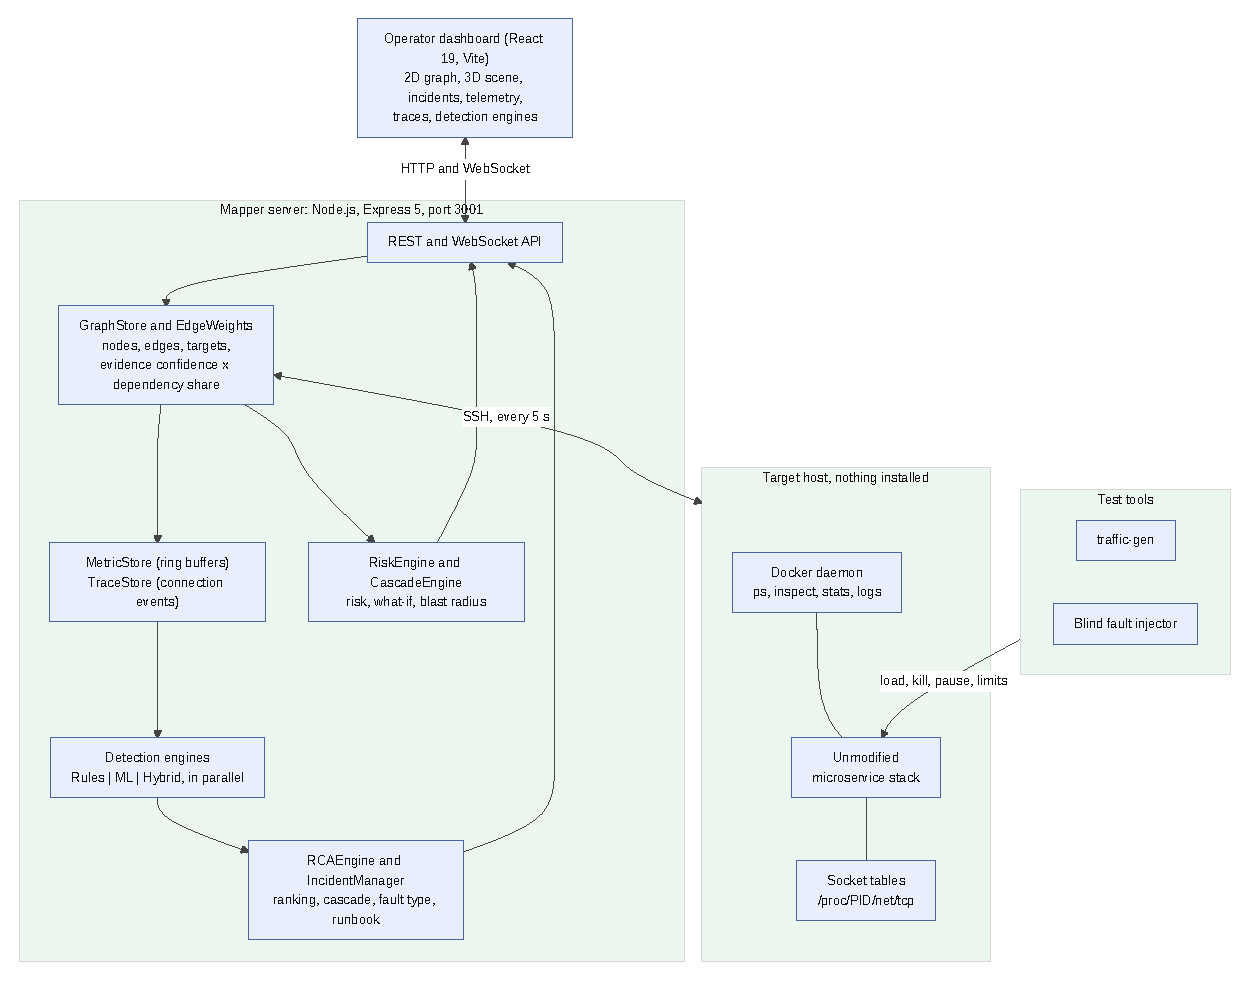
\includegraphics[width=0.98\textwidth,height=0.45\textheight,keepaspectratio]{d_architecture.pdf}
\caption{The architecture. The server reaches the target host over SSH and installs nothing on it. The three engines share the same readings and graph.}
\end{figure}

\section{The five layers, one sentence each}
\begin{center}
\small
\begin{tabularx}{\textwidth}{>{\raggedright\arraybackslash}p{3.1cm}>{\raggedright\arraybackslash}X}
\toprule
\textbf{Layer} & \textbf{What it is}\\
\midrule
Dashboard & A React 19 app. It never polls; the server pushes graph and incident updates over a WebSocket.\\
Server & One Node.js process (Express 5, TypeScript). It owns all state and is the only thing that writes to disk.\\
Connection and collection & One SSH session per target, running commands from a fixed, sanitised catalogue.\\
Target workloads & Unmodified Docker Compose applications. We touch nothing.\\
Test tools & A traffic generator and a blind fault injector, used for experiments only.\\
\bottomrule
\end{tabularx}
\end{center}

\section{The three engines and the switch}
\begin{simplebox}
At the top of the dashboard there is a switch: \textbf{Rules}, \textbf{Hybrid}, \textbf{ML}. These are three different ways of deciding that something is wrong. All three are always running in the background on the same data; the switch only chooses \emph{which one is allowed to open incidents}.

\begin{itemize}
\item \textbf{Rules} is the old-fashioned way: compare each number with the service's own recent history, and complain when it is far off. Fast, easy to explain, but it fires on ordinary noise and often blames the wrong service.
\item \textbf{ML} is our load-aware model plus the random walk. Fewest false alarms, best at naming the true source, but it needs about thirty readings per service before it judges anything.
\item \textbf{Hybrid} (the default) alarms if \emph{either} one alarms, or if a container is stopped, paused or crash-looping. It names the source with the ML ranking.
\end{itemize}
\end{simplebox}

\begin{techbox}
The Hybrid raises the alarm if a container fact holds ($\max_s f_s=1$), or the largest ML level reaches $\tau_\lambda=2$ (twice its own alarm line), or the largest rule score reaches $\tau_\rho=1.25$ (the rules alone must pass $1.25\times$ their own three-sigma line before they are trusted). A container fact raises the alarm at once. In the live system the model and rule conditions must hold for two consecutive windows. The offline evaluation requires two consecutive windows for all three conditions, the stricter reading. Ranking: services with a container fact first, then the ML random-walk order. Keeping all three engines computed on every cycle means that switching engines never starts the learned detector from nothing, and the Detection engines page can show what each decided, computed and predicted at the same moment.
\end{techbox}

\begin{figure}[H]
\centering
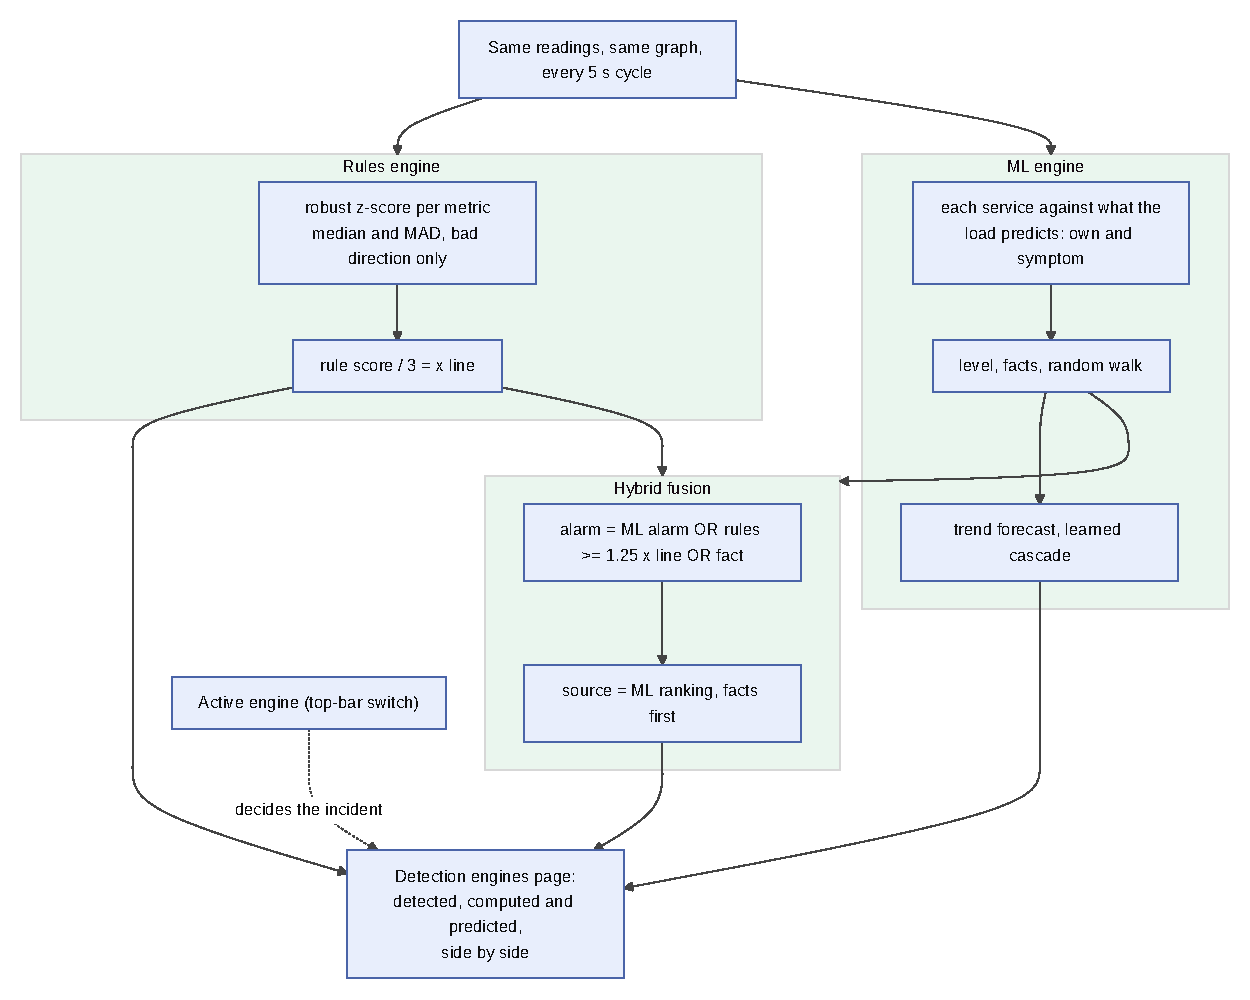
\includegraphics[width=0.98\textwidth,height=0.42\textheight,keepaspectratio]{d_engines_parallel.pdf}
\caption{The three engines run in parallel on the same inputs. The switch chooses which one decides the incident.}
\end{figure}

\begin{saybox}
``All three engines run all the time. The switch does not turn engines on or off; it chooses which one is allowed to open an incident. That is why the Detection engines page can compare them live on the same moment.''
\end{saybox}

\section{Design principles that explain odd-looking code}
Evaluators sometimes ask ``why is it done this strange way?'' The answer is almost always one of these rules.

\begin{enumerate}
\item \textbf{Nothing is installed on the target.} One SSH connection and a fixed set of Docker and \code{/proc} reads. The cost: no per-request data.
\item \textbf{Observed beats declared.} A \code{depends\_on} line is a claim; an open socket is a fact. The graph keeps both but never weighs them equally.
\item \textbf{Unmeasured is missing, never zero.} Zero means ``measured, and it was zero''. A made-up zero looks real on screen.
\item \textbf{Every number can be checked by hand.} Scores are arithmetic over named inputs, and the parts are shown.
\item \textbf{An arrow means ``calls''.} A failure moves \emph{against} the arrow. Reversing it flips everything downstream.
\item \textbf{Compare like with like.} Every model trains on one service's own history; degree, share and criticality are computed inside one project.
\item \textbf{Rules and models stay separate.} Incidents come from the detection engines; the optional Python findings are kept apart so no model is graded on its own output.
\item \textbf{Be light on the target.} Each loop waits for itself, reads each container once per sweep and rediscovers everything every 180 seconds.
\end{enumerate}

\begin{warnbox}
Principle 3 is the one people trip over. In the UI an unmeasured value shows as a dash, not as ``0\%''. If an evaluator sees a dash and asks why, this is the reason.
\end{warnbox}

\section{What happens when a host is slow or down}
\begin{simplebox}
Some machines are so busy that even the simple question ``what containers are running?'' takes a long time. On one overloaded two-gigabyte machine with eighteen heavy services, that question took 45 seconds. If we gave up after 10 seconds the whole machine would disappear from the map, which would look like a mapper bug. So we wait longer, and we built two small tools to tell the two cases apart: one checks the host step by step, the other prints what the mapper believes about it.
\end{simplebox}

\begin{techbox}
Timeouts are sized for a loaded host. \code{npm run check-host} walks one instance and stops at the first failure: port 22, key permissions, login, memory/load/disk, whether \code{docker} answers within 25 s, whether the application answers, which peers each front end calls, whether the mapper is up. \code{npm run mapper-edges} prints the target's status and last-seen time, its nodes and every edge with its evidence and last-seen time. Operational finding (Chapter~6 of the report): a host too small for its workload looks exactly like a mapper fault.
\end{techbox}

\chapter{Seeing a system without touching it}
\label{ch:observe}

\section{What ``from outside'' really means}
\begin{simplebox}
Imagine you want to know how busy a building is without going inside or asking anyone to wear a tracker. You can stand across the road and count people entering and leaving, see which windows are lit, and see which delivery vans stop at which door. You cannot read their private letters, but you learn a lot.

That is what the mapper does with a computer. It logs into the machine over SSH (like a remote terminal), and runs ordinary commands that Docker already offers: \emph{which containers exist}, \emph{how much CPU and memory each is using}, \emph{who is connected to whom}. Nothing is installed in the application. If you removed the mapper tomorrow, the application would not know it had ever been watched.
\end{simplebox}

\begin{techbox}
The connection manager keeps one SSH session per target (the \code{ssh2} library, no \code{ssh} binary needed) and runs commands from a fixed catalogue: \code{docker ps --no-trunc --format '{{json .}}'}, \code{docker inspect}, \code{docker stats --no-stream}, \code{docker logs}, and reads of \code{/proc/<pid>/net/tcp} and \code{/proc/<pid>/net/dev}. Every argument that reaches a shell passes a sanitiser (container identifiers must match the shapes Docker produces; timestamps and tail lengths are validated), and a test checks that an identifier with shell metacharacters is refused before any command is built. Each command has a timeout and a maximum output size.
\end{techbox}

\begin{saybox}
``The key sentence is: \emph{one SSH connection, a fixed list of read-only Docker and /proc commands, nothing installed.} That is why you can point it at a system you do not own.''
\end{saybox}

\section{The eight numbers per service}
\begin{simplebox}
For every service, every five seconds, we record eight numbers: how busy the processor is, how much memory it uses, how much it is being slowed down by its CPU limit (``throttling''), how much data comes in and goes out of its network, how many requests it handles, what share of them fail, and how slow the slowest ones are. That is the entire view we have. It is coarse, and we say so.
\end{simplebox}

\begin{techbox}
$x_s(t)=(\text{CPU},\ \text{memory},\ \text{throttle},\ \text{net in},\ \text{net out},\ \text{request rate},\ \text{error share},\ \text{p95 latency})$. CPU and memory are measured against the container's \emph{own} allowance, not the host's. Network counters come from the interface byte counters in \code{/proc/<pid>/net/dev}, which are exact, where \code{docker stats} prints values rounded to three significant figures (a 9.87\,MB counter moves in 10\,kB steps). Request rate, error share and latency exist only when a service reports them. A missing value stays missing.
\end{techbox}

\section{Who calls whom: the listening-port trick}
\begin{simplebox}
Every connection between two services is seen from \emph{both ends}. Service A shows a connection to B, and service B shows a connection from A. If you just record ``A talks to B'' on both sides, you get a fake arrow in each direction on every link, and the map becomes a tangle in which every service seems to depend on every other one.

The trick we use: on a connection, one side is the \emph{server} and holds a fixed ``listening port'' (like a shop's door number), and the other side is the \emph{client} and uses a random temporary port. The one with the fixed door number is the one being called. So the arrow points from the client to the owner of the listening port.
\end{simplebox}

\begin{techbox}
For each socket row in state ESTABLISHED or TIME\_WAIT: find the peer from the remote address (or apply the published-port rule when the call goes through the host's address). If the peer owns the remote port as a listening port and the scanned container does not own the local port, the edge is $a\to b$ with evidence \emph{listen-port}. If the scanned container owns the local port and the peer does not own the remote port, the edge is $b\to a$. If exactly one port is in the ephemeral range, the side with the ephemeral port is the caller (evidence \emph{ephemeral-port}). Otherwise the edge is marked \emph{unresolved} rather than guessed. Each connection is counted once by its key (caller ip:port $>$ callee ip:port), so a burst of short calls does not look like many links. Reading the socket table through the container's process id works for every image, including images with no shell.
\end{techbox}

\begin{examplebox}[A small worked example]
Suppose the \code{orders} container has an open connection from \code{10.0.0.5:51234} to \code{10.0.0.9:5432}. Which one is the database? Port 5432 is a well-known fixed port that the database container is listening on. Port 51234 is in the temporary range and no container is listening on it. So \code{orders} is the caller and the database is the callee, and the edge is $\texttt{orders}\to\texttt{orders-db}$ with evidence ``listen-port'' and confidence $1.0$.
\end{examplebox}

\begin{warnbox}
Before we fixed this, a bug recorded both directions for every link. Blast radius and criticality saturated: ``what is downstream of X?'' returned almost the whole graph. If an evaluator asks why we spend effort on direction, this is the answer: a wrong arrow flips every result that follows it.
\end{warnbox}

\section{Container facts: the things that are not ``a bit anomalous''}
\begin{simplebox}
If a container has stopped, that is not ``slightly unusual''. It is a fact, like a light being off. A normal statistics tool treats it as a very large anomaly score, which throws away the one thing you are sure about. We treat container state as evidence of its own kind. A container that is stopped, paused, restarting, or cut off from its network is a \emph{fact}, and when one exists, that service is ranked first.
\end{simplebox}

\begin{techbox}
\code{containerFact} maps the runtime state to \emph{down} (exited with a non-zero code, dead, vanished or not found), \emph{paused}, \emph{restarting}, \emph{detached} (network detached while running) or \emph{benign} (a load generator, or a container that exited with code 0). We added two facts that raw state misses after inspecting the real runs. First, \code{docker stop} exits with code zero, which looks like a finished job, so a service that had been running and then exits is marked \emph{stopped}. Second, a crash loop looks healthy between kills, so two outages within three minutes mark it. The ablation shows these facts matter most: removing the \code{docker stop} fact costs 18 points of caught-and-named on the real systems and 15 on the synthetic set.
\end{techbox}

\begin{saybox}
``Container state is a fact, not a degree. That single decision is worth more than any statistical refinement we tried. Remove the stop-fact and we lose 18 points on the real systems.''
\end{saybox}

\section{The one write the mapper makes}
\begin{simplebox}
Almost everything the mapper does is looking. The one thing it can \emph{do} is restart a container that crashed (exited with an error), a few times at most. It never touches containers that were stopped on purpose, and never restarts load generators. You can turn it off with one setting. We tested whether it changes our results by running the same faults with it on and off: it made no measurable difference on our two benches.
\end{simplebox}

\begin{techbox}
Setting: \code{MAPPER\_AUTO\_RESTART=off}. The rule skips exit code 0, so a deliberate \code{docker stop} is never undone. Live campaigns (21 faults each, auto-restart on and off, both benches) showed no effect beyond run-to-run variation, and a direct test (stopping \code{cart} and \code{payments} for 5 minutes each) showed the stopped containers stayed down for $\approx 300$\,s in both modes. Recommendation: switch it off when measuring detection, so the mapper cannot heal the faults the injector applies.
\end{techbox}

\chapter{The map: building and trusting the call graph}
\label{ch:graph}

\section{Two sources, two levels of trust}
\begin{simplebox}
There are two ways to know that service A depends on service B. One is that someone \emph{wrote it down}: the configuration file says ``A depends on B''. The other is that we \emph{saw it happen}: A really opened a connection to B a moment ago. Written-down links can be stale. Seen links are real, but a connection that is only seen once might be a fluke.

So we keep both, and we give every link a trust score between 0 and 1 based on how good its evidence is. A link we saw clearly, with a clear direction, gets 1.0. A link that exists only in the configuration file and never carried any traffic gets 0.4.
\end{simplebox}

\begin{techbox}
Declared edges come from the Compose file (\code{depends\_on}); observed edges come from socket tables. Each edge has a confidence $c(e)$ equal to its strongest evidence: $1.0$ for a call seen in request logs or oriented by a listening port; $0.85$ when only the ephemeral-port range orients it; $0.70$ observed without direction evidence; $0.50$ direction unresolved; $0.40$ declared but never seen carrying traffic. The dependency share $d(e)$ of an edge leaving a caller is its slow-baseline traffic normalised over that caller's edges. The edge weight is
\[
w(e)=\operatorname{clip}\bigl(c(e)\,d(e)\,\phi,\ 0,\ 1\bigr),
\]
with $\phi$ discounting fire-and-forget telemetry edges to a tenth. An observed edge expires ten minutes after it was last seen.
\end{techbox}

\begin{examplebox}[Why use a \emph{slow} baseline for the share?]
Suppose \code{orders} sends 90\% of its calls to \code{orders-db} and 10\% to \code{notifier}. Now \code{orders-db} dies. The traffic on that link drops to zero. If we weighted by the \emph{current} rate, the dead database would suddenly look unimportant to \code{orders} (0\% of traffic) at the exact moment it matters most. So the share is computed from a slow-moving average that remembers the link was important before it broke.
\end{examplebox}

\begin{warnbox}
The offline benchmarks replay recordings that do \emph{not} keep edge evidence, so they use unit weights. That means the report does \textbf{not} measure how much the evidence weighting helps. If an evaluator asks ``does the confidence weighting improve accuracy?'', the honest answer is: we use it live and it is consistent with what we saw, but we did not isolate its effect offline. That is listed under limitations and future work.
\end{warnbox}

\section{When names help, and when they do not}
\begin{simplebox}
Sometimes the listening-port trick cannot decide who calls whom. In those cases a simple fallback is to read the names: a service called ``gateway'' probably calls ``orders'', and ``orders'' probably calls ``orders-db''. That works until someone names their services ``alpha'', ``bravo'', ``charlie''. So we also built a version that learns the direction from how the services \emph{behave} when something goes wrong, with no help from names. When names are useless, it still gets 27 of 31 pairs right, where the name-based rule gets none right. When names are informative, the name-based rule is just as good, and we say so.
\end{simplebox}

\begin{techbox}
The collector sees most pairs from both ends (in the recorded runs 15 of 32 pairs in one system and 18 of 36 in the other), so direction must be recovered before a walk can follow it. The shipped heuristic reads names (an entry point calls a service, a service calls a datastore). Learned directions use four \emph{dynamic} signals (upward symptoms, downward traffic drops, implication $P(T_a\mid T_b)-P(T_b\mid T_a)$ with $T$ meaning ``in trouble'', and a Granger-style F-test on the symptom series) and two \emph{structural} signals (each service's depth from the entry point, and whether it reports request metrics of its own, which a datastore does not). The learned direction is the sign of $\sum_m\omega_m s_m(a,b)$ with weights $\omega_m\in\{0.5,1,2\}$ chosen by grid search on the tuning split; a pair stays undecided if the magnitude falls below $0.05$.
\end{techbox}

\begin{saybox}
``Learned directions stay correct when service names carry no information, 27 of 31 pairs against none for the name rule. But we are not claiming they improve ranking when names exist. They do not. We report that.''
\end{saybox}

\section{Why direction decides everything downstream}
\begin{simplebox}
Think of a river map. If you draw the arrows backwards, ``what is downstream of the factory?'' gives you the towns upstream of it. Every question we ask later (which service is the likely origin, which services are next, what is the blast radius of this one failing) is a question about arrows. A wrong arrow does not make the answer slightly worse. It makes it the opposite.
\end{simplebox}

\begin{techbox}
An edge $A\to B$ means $A$ calls $B$, so a failure at $B$ hits $A$: failure propagates \emph{against} the arrow. The random walk, the cascade risk and the blast radius all traverse the graph along or against edges. In the first version of the observation layer the graph was effectively undirected (every pair got a cycle), so ``downstream of $X$'' reached almost everything and blast radius and criticality saturated. A test now guards the orientation logic.
\end{techbox}

\chapter{Deciding that a service is behaving abnormally}
\label{ch:detect}

\section{The core idea: normal is personal}
\begin{simplebox}
What is a normal number? It depends on who you ask. A database might use 40\% of its memory all day, and that is normal for it. A tiny helper service might use 2\%. A rule such as ``alarm if memory is over 80\%'' is wrong for both of them. So instead of one rule for everyone, we compare every service with \emph{its own recent past}. If the database suddenly uses 90\% when it usually uses 40\%, that is unusual \emph{for the database}.
\end{simplebox}

\begin{techbox}
Services differ by orders of magnitude in every metric, so global thresholds fail. Each service is judged against its own recent window of readings, using robust statistics: the median for location and the median absolute deviation (MAD) for spread, because a mean and standard deviation are dragged by the very outliers we are trying to detect. A robust $z$ is $(x-\operatorname{median})/(1.4826\cdot\mathrm{MAD})$, and the constant 1.4826 makes MAD comparable to a standard deviation for Gaussian data.
\end{techbox}

\section{Engine 1: the rules}
\begin{simplebox}
The rule engine is the simple one. For each of the eight numbers it asks ``how many robust standard deviations away from this service's normal is it right now?'' and only cares about the bad direction (CPU going up, not down). If that distance passes a line (three), the service is flagged. Container facts (stopped, paused, crash-looping) are also flagged outright.

Strengths: very easy to explain, reacts fast to loud faults. Weaknesses: it fires on ordinary noise, so it raises the most false alarms, and it blames the loudest service, which is often a victim.
\end{simplebox}

\begin{techbox}
A robust one-sided $z$-score per metric (median and MAD, bad direction only) gives a rule score $\rho_s$ normalised so that $1$ is its three-sigma line. Settings include \code{minHistorySamples}=12, \code{zScoreAnomaly}=3.5, \code{zScoreHigh}=5, \code{zScoreCritical}=8, \code{minDeltaPercent}=5 (a large $z$ is ignored unless the metric moved at least 5 percentage points, so an idle service going from 0.05\% to 2\% CPU does not raise an incident), and absolute thresholds of 70\% (high) and 85\% (critical) for CPU and memory. Measured on the 62 real faults the rules detect 90\%, catch-and-name 63\%, raise 9.2 false-alarm episodes per fault-free hour and spend 9\% of the time in alarm.
\end{techbox}

\section{Engine 2: the old ML, an Isolation Forest per service}
\begin{simplebox}
An Isolation Forest is a way to find ``odd one out'' points. Imagine a pile of marbles on a table. If you draw random lines through the pile, a marble sitting far from the pile gets separated from the rest after only a few lines, while a marble in the middle takes many cuts. The fewer cuts it takes to isolate a point, the more unusual it is.

We trained two of these per service on its recent readings. They are good at ``this reading is unlike the recent ones''. And that is exactly their weakness: when the \emph{whole system} gets quieter, every service's readings are unlike the recent ones, so everything looks odd at once.
\end{simplebox}

\begin{techbox}
Isolation Forest (Liu, Ting and Zhou, 2008) isolates an outlier with few random cuts, with the anomaly score a monotone function of the expected path length. It needs no density estimate, which suits mixed, skewed metrics. The first engine used two forests per service (one over ``own'' resource signals, one over ``symptom'' signals), plus a range guard, and a 30-minute wait before accepting a large shift as the new normal. A forest cannot score a value beyond its training range higher than its most extreme training point, so the engine added a range guard; but that guard fires for every service when traffic changes for all of them.
\end{techbox}

\section{Engine 3: the new ML, the load-aware residual model}
\label{sec:loadmodel}
This is the part to understand best, because it is the contribution that came out of the failure.

\subsection{Step 0: the picture}
\begin{simplebox}
Imagine ten shops on one street. On a rainy day, every shop gets fewer customers. If you check each shop separately against its own history, every shop looks ``abnormally quiet'' and you think ten shops are broken. A smarter check first asks: \emph{how quiet is the whole street?} If the street is down by half, you expect every shop to be down by about half. Then you look for the shop that is down by \emph{more} than half, or the one that is up when the others are down. \emph{That} shop has a real problem.

This is the entire idea. Estimate the shared change, expect each service to follow it, and look at the leftover.
\end{simplebox}

\subsection{Step 1: put numbers on a log scale}
\begin{simplebox}
Traffic changes are multiplicative: ``twice as busy'' matters whether the service handled ten requests or ten thousand. A log scale turns ``twice as much'' into the same step everywhere. We also add a small ``unit'' so that tiny flickers on an idle service (a 1\% CPU blip) do not look like big events.
\end{simplebox}

\begin{techbox}
Each signal is $x_{s,f}=\log(v_{s,f}+u_f)$ with units $u_f=5$ for CPU (so a one-point blip on an idle service is no event), $1$ for memory, $2000$\,B/s for network and $0.1$ for request rate. A missing signal stays missing.
\end{techbox}

\subsection{Step 2: a slow reference}
\begin{simplebox}
For each number of each service we keep a ``reference'': the typical value over the last half hour. We take the \emph{median} (the middle value), not the average, so one weird spike does not move it. Everything is then measured as ``how far above or below its own reference is it right now?''
\end{simplebox}

\begin{techbox}
$r_{s,f}$ is the median of the service's last $360$ readings (half an hour at 5\,s). A short quiet spell does not move it. The shift is $d_{s,f}(t)=x_{s,f}(t)-r_{s,f}$.
\end{techbox}

\subsection{Step 3: measure the shared change (the load factor)}
\begin{simplebox}
Now take all the services that carry traffic and ask: on average, how far have they all moved right now? Use the \emph{median} of their moves. A median is the middle one when you line them up. If one service goes crazy, it is only one number at the end of the line, and the middle barely moves. If \emph{every} service moves up, the middle moves up. That is exactly the behaviour we want: the load factor follows the shared change and ignores a single broken service.

An idle database that always reads zero says nothing about traffic, so we only use signals that actually carry traffic (their reference is clearly above idle).
\end{simplebox}

\begin{techbox}
A signal \emph{carries traffic} if $r_{s,f}-\log u_f\ge 0.4$. Over the carrying signals of network in/out, request rate and CPU, the load factor is
\[
L(t)=\operatorname*{median}_{(s,f)\in\mathcal A(t)}\ d_{s,f}(t),
\]
taken only when at least two services contribute. $e^{L}$ is the factor by which the project's traffic changed; the Detection engines page shows it as a chip (``workload steady'' or ``traffic $\times$2.4, explained, not a fault'').
\end{techbox}

\begin{examplebox}[Worked example: ten services, one broken]
Nine busy services each move by about $+0.7$ on the log scale (traffic roughly doubled; $e^{0.7}\approx2$). One service, \code{payment}, moves by $+3.0$ because it is also in trouble. Sort the ten moves: $0.6,0.65,0.7,0.7,0.7,0.7,0.75,0.8,0.85,3.0$. The median is the average of the 5th and 6th, $(0.7+0.7)/2=0.7$. The load factor is $0.7$, not dragged by \code{payment}'s $3.0$. Expected move for each service is about $0.7$. \code{payment}'s leftover is $3.0-0.7=2.3$, which is large; the others' leftovers are about $0.0$ to $0.15$. Only \code{payment} stands out.
\end{examplebox}

\subsection{Step 4: some signals follow the load, some ignore it}
\begin{simplebox}
Not everything follows traffic. A gateway's network use goes up with traffic. A message bus idling in the corner may stay the same. The mapper learns, for each kind of signal, how strongly it follows the shared change in \emph{this} project, by comparing the past shared change with the past movement of those signals. If it has not seen enough load changes to learn, it uses a sensible starting guess (network and requests follow load about one-for-one, CPU about 0.4).
\end{simplebox}

\begin{techbox}
The slope $b_f$ is a ridge regression of the shifts $d_{s,f}(\tau)$ on $L(\tau)$ over the carrying signals in the stored window:
\[
b_f=\frac{\sum d\,L+\kappa\,b^0_f}{\sum L^2+\kappa},\qquad \kappa=60,
\]
with priors $b^0=1$ for network and requests and $0.4$ for CPU. The ridge term pulls the slope towards the prior until the data say otherwise.
\end{techbox}

\subsection{Step 5: judge the leftover, under two excuses}
\begin{simplebox}
Here is the clever safety trick. For each number we try two excuses. Excuse one: ``this signal ignores the load'' (so expect no change). Excuse two: ``this signal follows the load'' (so expect it to have moved with the street). If \emph{either} excuse explains the reading, it is not unusual. A reading is flagged only if \emph{neither} excuse can explain it. This keeps us from raising false alarms while the load changes, and keeps us from missing a real fault that happens during a load change: a CPU spike on one service during a traffic surge is still a spike compared with what the surge predicts.
\end{simplebox}

\begin{techbox}
For each hypothesis $b\in\{0,b_f\}$, the window of the service's \emph{accepted} readings gives a baseline $m^{(b)}$ (the median of $x_{s,f}(\tau)-bL(\tau)$) and a robust spread $\sigma^{(b)}$. The deviation is
\[
z_{s,f}=\min_{b\in\{0,\,b_f\}}\ \frac{\lvert x_{s,f}-bL-m^{(b)}\rvert}{\sigma^{(b)}},
\]
so a signal counts as unusual only if neither way of following the load explains it. Only \emph{increases} of CPU, memory, throttling, errors and latency count (less of them never signals a fault of the service itself and follows every restart); traffic counts in both directions. The service's level is $\max_f z_{s,f}/z_{\text{line}}$ with $z_{\text{line}}=4$, so level $1$ is the service's own alarm line and the hybrid uses level $2$ ($z=8$). The strongest signal and its $z$ are kept, so the verdict reads ``CPU 9.3 spreads from what the load predicts''.
\end{techbox}

\subsection{Step 6: how wide is ``normal''? The tail-aware spread}
\begin{simplebox}
Some numbers are \emph{bursty}: they are quiet most of the time and jump every few minutes even when nothing is wrong (think batch jobs). If you measure the spread of such a number in the usual way, the spread looks tiny, so an ordinary burst looks like a five-alarm event. We fix this by making the spread at least as wide as the distance from the typical value to the 90th-percentile value, in the direction we care about. A burst that happens regularly is then part of the normal width.
\end{simplebox}

\begin{techbox}
$\sigma=\max\bigl(1.4826\,\mathrm{MAD},\ (q_{0.90}-m)/1.2816,\ \phi_f\bigr)$ for the upper tail, or both tails for two-sided signals, with a floor $\phi_f$ at the smallest change worth noticing (floors $[0.2,0.05,0.3,0.3,0.3,0.02,0.2,3]$ over the eight signals). The MAD alone treats a bursty signal as Gaussian and alarms on its ordinary bursts. Measured effect: with the MAD spread instead of the tail-aware one, alarm time on the workload recordings rises from 0\% to 10\% and 6\%, and on the real systems it doubles from 6\% to 12\%.
\end{techbox}

\subsection{Step 7: do not learn from your own alarms}
\begin{simplebox}
The model learns what normal looks like from recent readings, but with a rule: \emph{only readings that were not alarming are allowed into the learning window.} Otherwise a long fault would slowly teach the model that the fault is normal, and the alarm would fade. There is one exception, on purpose. If a service settles at a new level that is only slightly unusual, and stays there for two minutes, we accept it as the new normal. A big shift is only accepted after thirty minutes. This way a service that really did change (after a deploy, say) stops alarming forever, but a real fault does not get absorbed quickly.
\end{simplebox}

\begin{techbox}
Only readings under level $1$ join the window of $W=120$ readings. A small steady shift (level below $3$) is accepted as the new normal after $24$ readings (two minutes), a large one after $360$ (thirty minutes). A service is judged only after $30$ readings. Baselines are cached and refreshed every four readings. The price: a mild fault that lasts longer than two minutes is eventually absorbed and the model stops alarming on it, while the rule layer and the container facts of the hybrid keep alarming. Raising the two-minute setting to 4--20 minutes changed nothing on accuracy but doubled alarm time on the real systems from 6\% to 13\%, so we kept two minutes.
\end{techbox}

\begin{warnbox}
This absorbed-fault behaviour is a real limitation, and you will see it in the live demo of the simulator: the ML engine alarms on the slow \code{payment} fault for about 48 simulated seconds, then goes quiet, while the Rules and Hybrid keep alarming. Say so before an evaluator notices it.
\end{warnbox}

\subsection{Summary of the model in one picture}
\begin{figure}[H]
\centering
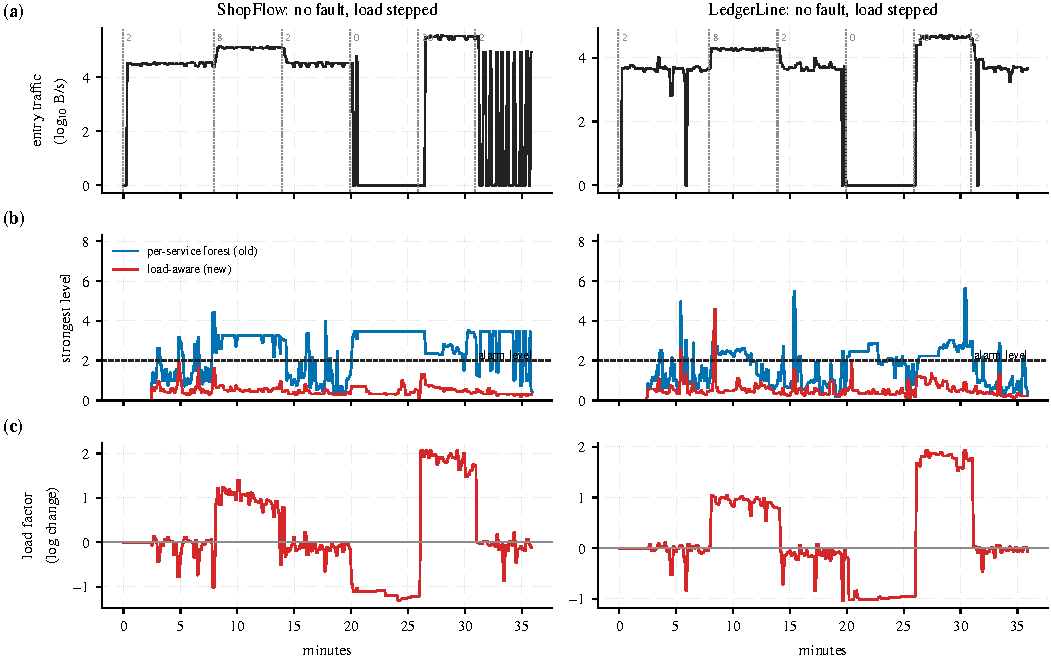
\includegraphics[width=0.98\textwidth]{fig_workload.pdf}
\caption{Two fault-free recordings with the load stepped (left ShopFlow, right LedgerLine). (a) Network traffic into the entry service. (b) The strongest service level of the old forest and of the load-aware model; the dashed line is the alarm level. (c) The load factor the new model read.}
\end{figure}

\begin{saybox}
``Panel (a) is the traffic going up and down. Panel (b) is the key: the old forest's level goes high every time the traffic changes, while the new model stays flat under the line. Panel (c) is why: the load factor follows the steps, so the model \emph{explains} the change instead of calling it a fault.''
\end{saybox}

\section{Hybrid: why have all three}
\begin{simplebox}
Rules react fast but fire on noise. ML is quiet and good at naming the source, but it needs warm-up and can absorb a slow fault. Container facts are the most reliable signal of all. The Hybrid alarms if \emph{any} of the three says so, and names the source using the ML ranking. We tuned one number: the rules alone only count if they go 25\% past their own line, so the Hybrid does not inherit all of the rule engine's false alarms.
\end{simplebox}

\chapter{The ML correction: what went wrong and how we fixed it}
\label{ch:mlstory}

This part is the longest on purpose. If the evaluator asks only one hard question, it will be about the ML, and the best answer is the true story told in order.

\section{The timeline}
\begin{enumerate}
\item \textbf{Version 1.} A per-service Isolation Forest, a random walk to rank causes, a hybrid with the rules. It scored well on our injected-fault benchmarks.
\item \textbf{The report.} Stopping the traffic generator and switching to ML made \emph{every service show a 100\% anomaly score}. Nothing was broken.
\item \textbf{Reproducing it.} We recorded fault-free runs where only the workload changed. In the first set the organic traffic generator ran, stopped, ran, stopped for longer, and ran again (62 minutes). In the second, a closed-loop generator held a constant number of visitors and stepped it $2\to8\to2\to0\to20\to2$ (72 minutes). Every alarm in those recordings is a false alarm by construction.
\item \textbf{The benchmark had hidden it.} Our replay tool skipped a reading whenever it was identical to the previous one. An idle service reports the same zeros again and again, so the replay deleted the idle stretches, and the old forest looked well behaved when traffic stopped. We fixed the replay.
\item \textbf{Comparing alternatives.} We built the contenders (below) and measured them on injected faults \emph{and} on those fault-free recordings.
\item \textbf{The choice.} The load-aware residual model with a tail-aware spread.
\item \textbf{Adopting and re-running everything.} Made the default, re-ran every experiment, tests, figures and the report.
\end{enumerate}

\begin{saybox}
Tell it in this order. The shape is: \emph{we found a real failure, we reproduced it, we found out why our own benchmark had hidden it, we compared fixes fairly, we picked the one that worked, we re-ran everything.} That is a strong research story.
\end{saybox}

\section{Why the old engine failed, in one picture}
\begin{simplebox}
The forest learned the \emph{shape} of each service's recent numbers. When the traffic changed, the numbers moved to a place the forest had never seen, for all services at once. A forest cannot say ``this is just louder than before''; it only knows ``this is unlike what I have seen''. Add a safety guard that fires when a value falls outside the range seen so far, and a total traffic change makes every guard fire at the same time. On top of that, a big shift was only accepted as the new normal after thirty minutes.
\end{simplebox}

\begin{techbox}
On fault-free workload recordings the old forest was in alarm 23\% (organic on/off) and 52\% (stepped load) of the time, and raised 27.7 and 21.3 false-alarm episodes per hour. Every other workload-blind detector did the same or worse: the ensemble of four 47\% and 88\%, k-NN 73\% and 96\%, Mahalanobis 38\% and 76\%, HBOS 75\% and 82\%. Because all of them model the readings themselves, a new workload is outside what they were fitted on. A forest also scores a value beyond its training range no higher than its most extreme training point, so the engine had added a range guard, which fires at once for every service when traffic changes for all of them. On the fault-free stretches of the live fault campaigns the same engine raised 40.9 alarm episodes per hour.
\end{techbox}

\section{The contenders}
\begin{simplebox}
We tried several ways of fixing it, so nobody could say we just picked the first thing. Three families:

\begin{enumerate}
\item \textbf{More of the same.} Other ``learn the shape'' detectors (k-NN, Mahalanobis, HBOS, an ensemble). They fail the same way.
\item \textbf{Simple control chart.} Judge each number against its own history with robust statistics, no learned shape. This already helps a lot, because it does not claim to know the shape of traffic.
\item \textbf{Ones that treat the shared workload explicitly.} A subspace model (the classic multivariate monitoring idea: the shared cause is one or two ``directions'' in the data, and an anomaly is what falls off those directions), and our load-factor model.
\end{enumerate}
\end{simplebox}

\begin{techbox}
All unsupervised, all computed from telemetry the mapper already collects. (a) Forest family: Isolation Forest, ensemble, k-NN, Mahalanobis, HBOS. (b) Control chart with MAD spread or tail spread. (c) Subspace residual (principal-component residual of the standardised readings of all services, 1 or 2 components). (d) Load factor with MAD or tail spread. We also tried and rejected a range guard on the residual (it added false alarms and changed no injected-fault result) and varied the alarm line, window, slow reference and drift time.
\end{techbox}

\section{The results table, and how to read it}
\begin{figure}[H]
\centering
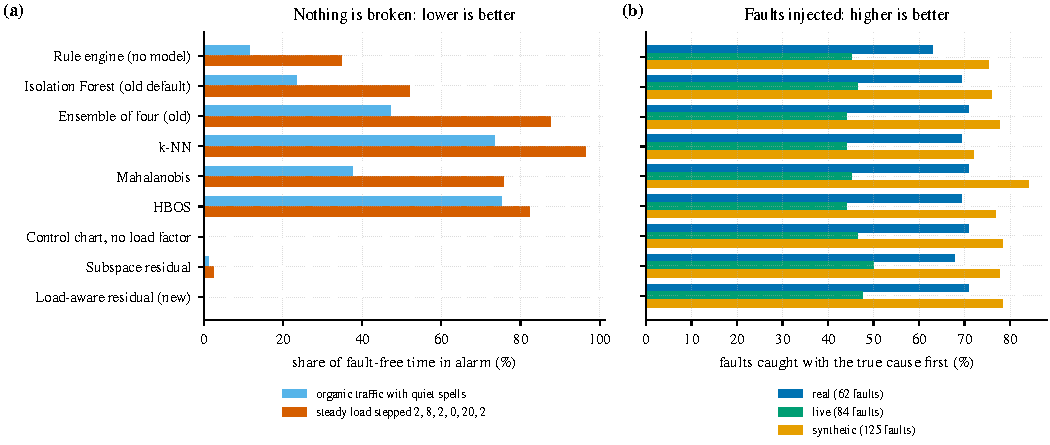
\includegraphics[width=0.98\textwidth]{fig_models.pdf}
\caption{The candidate models. (a) Share of fault-free time in alarm on the two workload recordings (lower is better). (b) Share of injected faults caught with the true cause first (higher is better).}
\end{figure}

\begin{center}
\scriptsize
\setlength{\tabcolsep}{3pt}
\begin{tabular}{lrrrrrrrr}
\toprule
 & \multicolumn{2}{c}{Real (62)} & \multicolumn{2}{c}{Live (84)} & \multicolumn{2}{c}{Synthetic (125)} & \multicolumn{2}{c}{No faults}\\
Model & C+N & FA/h & C+N & FA/h & C+N & FA/h & organic & steps\\
\midrule
Rule engine (z-score) & 63 & 9.2 & 45 & 16.3 & 75 & 2.6 & 12 & 35\\
Isolation Forest (old) & 69 & 4.6 & 46 & 40.9 & 76 & 0.2 & 23 & 52\\
Ensemble of four & 71 & 20.0 & 44 & 81.7 & 78 & 2.6 & 47 & 88\\
k-NN & 69 & 13.8 & 44 & 57.2 & 72 & 5.2 & 73 & 96\\
Mahalanobis & 71 & 23.8 & 45 & 65.4 & 84 & 2.6 & 38 & 76\\
HBOS & 69 & 34.6 & 44 & 57.2 & 77 & 1.4 & 75 & 82\\
Control chart, MAD spread & 73 & 10.0 & 44 & 24.5 & 79 & 0.6 & 13 & 31\\
Control chart, tail spread & 71 & 2.3 & 46 & 0.0 & 78 & 0.2 & 0 & 0\\
Subspace residual, 1 comp. & 68 & 3.1 & 50 & 8.2 & 78 & 0.4 & 1 & 3\\
Subspace residual, 2 comp. & 68 & 3.8 & 50 & 0.0 & 77 & 0.2 & 1 & 4\\
Load factor, MAD spread & 71 & 3.8 & 43 & 16.3 & 79 & 0.6 & 10 & 6\\
\textbf{Load factor, tail spread} & 71 & 2.3 & 48 & 0.0 & 78 & 0.2 & 0 & 0\\
\bottomrule
\end{tabular}
\end{center}

\begin{simplebox}
How to read this table in thirty seconds. \textbf{C+N} is ``caught and named'': the fault was detected \emph{and} the correct service was ranked first, in percent (higher is better). \textbf{FA/h} is false alarms per hour of fault-free time (lower is better). The last two columns are the share of time spent in alarm on recordings where \emph{nothing was broken}; every minute in alarm there is a mistake (lower is better, zero is perfect).

Look at the last two columns first: the forest family is at 23--96\%, the adopted model at 0\%. Then look at the C+N columns: they are all close, 68--84\% on the real and synthetic sets, 43--50\% on the live sets. So \emph{the models are alike at catching faults; they are not alike at staying quiet when only the workload moves.}
\end{simplebox}

\begin{techbox}
Three results stand out. (1) On injected faults the models are alike (68--73\% real, 43--50\% live, 72--84\% synthetic); differences of a few points are inside the noise of 62--125 faults. The forest-family detectors raise 4.6--34.6 episodes/h on the real systems and 40.9--81.7 on the live ones, against 2.3 and 0.0 for the adopted model. (2) On workload shifts they differ: adopted 0\% and 0\%, workload-blind family 23--75\% and 52--96\%. Replacing the forests by a robust residual with the tail-aware spread is the larger part of the improvement (control chart: 0\% and 0\%); the MAD spread alone is not enough (13\% and 31\%) because it treats bursty signals as Gaussian. (3) The load factor removes what is left: the control chart still raises 1.2 and 1.9 false episodes/h on the two recordings; with the load factor 0.0 and 1.0, and it is slightly better on the live faults (47.6\% against 46.4\% caught and named). The subspace residual is the strongest alternative (3\% and 4\% of the steady recording in alarm; 50\% C+N on live faults) but raises 7.7--10.7 false episodes/h on the steady steps, adapts more slowly and its cost grows faster than linearly.
\end{techbox}

\begin{warnbox}
Be honest about what the new model is \emph{not}: it is not more accurate than the forest at catching injected faults (71\% against 69\% on the real faults, inside the noise). The benefit is robustness: it does not mistake a workload change for a fault. Also admit that a fault that begins during a very large change of load can be masked, because both load hypotheses may explain it.
\end{warnbox}

\section{How we set its dials, and what each does}
\begin{center}
\small
\begin{tabularx}{\textwidth}{>{\raggedright\arraybackslash}p{4cm}>{\raggedright\arraybackslash}p{2.4cm}>{\raggedright\arraybackslash}X}
\toprule
\textbf{Dial} & \textbf{Value} & \textbf{What it does, in plain words}\\
\midrule
Alarm line $z_{\text{line}}$ & 4 robust spreads & How far from normal counts as ``level 1''. Looser (2) catches more faults but alarms on workloads; tighter (6--8) is silent but loses detection. 4 is the loosest value that keeps the workload recordings quiet.\\
Training window & 120 readings & About ten minutes of normal behaviour to learn from. 60 is too short (noisy again).\\
Slow reference & 360 readings & The half-hour median that shifts are measured from.\\
Readings before judging & 30 & Warm-up per service.\\
Mild drift & 24 readings & A small steady change becomes normal after 2 minutes.\\
Large drift & 360 readings & A large change needs 30 minutes.\\
Alarm level & 2 & The hybrid needs twice the line.\\
Persistence & 2 windows & The alarm must hold on two cycles in a row.\\
\bottomrule
\end{tabularx}
\end{center}

\begin{figure}[H]
\centering
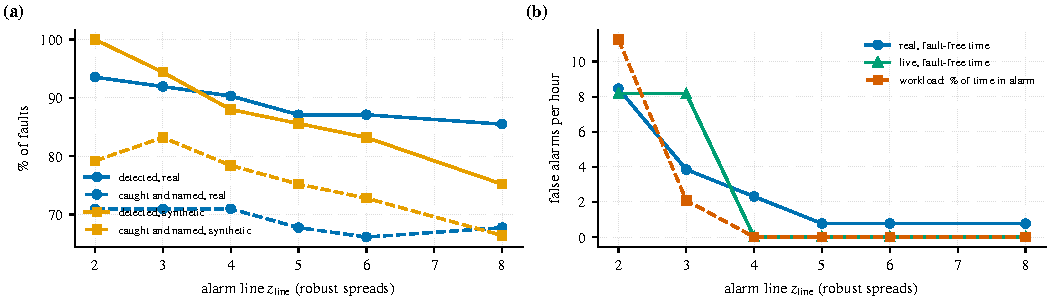
\includegraphics[width=0.98\textwidth]{fig_zline.pdf}
\caption{Sensitivity of the load-aware model to its alarm line.}
\end{figure}

\begin{warnbox}
We swept these dials on all recordings together. That is tuning on the test data, and the report says so. We chose the flat region of the sweep, not its maximum. If asked ``did you overfit the settings?'', say: ``Partly possible. The synthetic results come from a split we tuned on separately and scored once; the real-system numbers have no held-out system, so they are optimistic by an amount we cannot measure.''
\end{warnbox}

\section{The three-way comparison document}
We also wrote a standalone comparison in the repository (\code{wiki/44-ml-comparison.md}) that puts Rules, the old ML and the new ML side by side with plain-language reasons. Section 6.1.3 and Table 6.2 of the report show the same thing. The headline from it:

\begin{center}
\small
\begin{tabular}{lccc}
\toprule
 & Rules & Old ML & New ML\\
\midrule
Real faults: C+N / FA per h & 63\% / 9.2 & 69\% / 4.6 & \textbf{71\% / 2.3}\\
Live faults: C+N / FA per h & 45\% / 16.3 & 46\% / 40.9 & \textbf{48\% / 0.0}\\
Synthetic: C+N / FA per h & 75\% / 2.6 & 76\% / 0.2 & \textbf{78\% / 0.2}\\
Time in alarm, traffic on/off & 12\% & 23\% & \textbf{0\%}\\
Time in alarm, stepped load & 35\% & 52\% & \textbf{0\%}\\
Cost, 320 services (ms) & -- & 296 & \textbf{119}\\
\bottomrule
\end{tabular}
\end{center}

\begin{techbox}
Per-reading ranking (ROC): the plain rule $z$-score has the best AUROC on both sets (0.695 real, 0.873 synthetic) against 0.629 and 0.862 for the old forest and 0.665 and 0.842 for the load-aware model; the load-aware model has a higher average precision than the forest on the held-out set (0.665 against 0.528). This is not a contradiction: one high reading is cheap. What the user sees is an alarm (two cycles in a row) and a named source, and there the rules fall behind because they fire on traffic swings and blame the loudest service.
\end{techbox}

\begin{saybox}
``Honestly, per single reading the plain rule score is the best classifier. We say that in the report. The new model is not adopted because it ranks single readings better. It is adopted because it stays quiet when only the workload moves, which is the failure that an operator actually hit.''
\end{saybox}

\chapter{ML deep dive A: the old model, step by step}
\label{ch:deepforest}

This part opens the old engine completely. You need it for two reasons. An evaluator who hears ``we replaced our Isolation Forest'' will ask ``what exactly did it do, and why did it fail?'' And understanding the old model is the fastest way to understand the new one, because every design choice in the new model answers a specific weakness here.

Everything below is taken from the source files \code{isolationForest.ts}, \code{serviceBaseline.ts} and \code{detectors.ts}.

\section{What the old engine did, in one paragraph}
\begin{simplebox}
For \emph{each service separately}, the engine kept a window of that service's recent ``normal'' readings (the last 120 that did not look wrong). Every ten new normal readings it trained fresh Isolation Forests on that window. A new reading was scored by the forests: ``how unlike the recent normal readings is this one?'' The score was turned into a level, where 0 means typical, 1 means ``on the alarm line'' and 2 means ``twice as far out as the line''. If a service's level stayed at or above 1 for two readings in a row, it counted as anomalous, and its level fed the random walk that picks the root cause.
\end{simplebox}

\section{The Isolation Forest, with a tiny worked example}
\begin{simplebox}
Take a dozen people standing in a room, and ask each person their height. Now play the ``twenty questions'' game with random questions: pick a random cut, say ``are you taller than 1.63\,m?'', and split the room. Keep asking random questions to each half until every person stands alone. A very tall person (2.10\,m) is likely to be alone after one or two random cuts. A person of ordinary height needs many more cuts before they are alone, because many others look like them. \emph{The number of cuts needed to isolate a point is a measure of how unusual the point is.} An Isolation Forest repeats this with many random trees and averages the number of cuts.
\end{simplebox}

\begin{techbox}
Each tree is grown on a random sample of $\psi=64$ readings. At each node, among the features that still vary, one is chosen at random, and a random cut value is drawn uniformly between the minimum and maximum of that feature among the points at the node. The tree stops at depth $\lceil\log_2\psi\rceil=6$ or when one point is left. For a new reading $x$, the path length $h(x)$ is the depth at which it lands, plus a correction $c(n)$ for the number of points left at that leaf. The anomaly score is
\[
s(x)=2^{-\,E[h(x)]/c(\psi)},\qquad c(n)=2\bigl(\ln(n-1)+0.5772\bigr)-\frac{2(n-1)}{n}.
\]
$E[h(x)]$ is the average path over 100 trees. Here $c(64)=7.47$.
\end{techbox}

\begin{examplebox}[Check the formula]
With $\psi=64$ we have $c(64)=7.47$. If a reading is isolated after an average of only 2 cuts, its score is $2^{-2/7.47}=0.83$ (isolated fast: anomalous). If it takes about 7.47 cuts (an ordinary reading), the score is $2^{-1}=0.50$. If it takes 10 cuts, the score is $0.40$ (deep in the crowd).

\begin{center}
\small
\begin{tabular}{lcccccc}
\toprule
Average cuts $E[h]$ & 2 & 3 & 4 & 6 & 7.47 & 10\\
Score $s=2^{-E[h]/7.47}$ & 0.83 & 0.76 & 0.69 & 0.57 & 0.50 & 0.40\\
\bottomrule
\end{tabular}
\end{center}
So scores near 0.5 or below are ordinary and scores near 1 are anomalous.
\end{examplebox}

\section{From a raw score to a ``level''}
\begin{simplebox}
The raw score has no universal meaning: a quiet service and a busy service have different typical scores. So the engine learns each service's own scale. It scores all 120 of that service's own training readings. The median of those scores is ``typical''. The spread of those scores (the MAD, from Part~\ref{ch:primer}) is the natural wobble. The alarm line is set at ``typical plus three wobbles''. A new reading's level is how far its score is from typical, measured in units of the gap between typical and the line.
\end{simplebox}

\begin{techbox}
For each group of features: $\text{typical}=\operatorname{median}(s_i)$, $\text{spread}=1.4826\cdot\operatorname{MAD}(s_i)$, $\text{line}=\max(\text{typical}+3\cdot\text{spread},\ \text{typical}+0.02)$ for the forest (the margin of $0.02$ stops a perfectly flat series from alarming on noise). The level of a reading is $\max\bigl(0,\ (s-\text{typical})/(\text{line}-\text{typical})\bigr)$.
\end{techbox}

\begin{examplebox}[Worked example of a level]
Suppose the service's training scores have median $0.50$ and spread $0.02$. The line is $0.50+3\times0.02=0.56$. Now a new reading arrives:

\begin{center}
\small
\begin{tabular}{lccccc}
\toprule
Score of the new reading & 0.50 & 0.52 & 0.56 & 0.62 & 0.70\\
Level $=(s-0.50)/0.06$ & 0.00 & 0.33 & 1.00 & 2.00 & 3.33\\
\bottomrule
\end{tabular}
\end{center}
A level of 1 is the alarm line. A level of 2 is what the Hybrid needs to alarm.
\end{examplebox}

\section{The details that made the old engine behave the way it did}
\begin{center}
\small
\begin{tabularx}{\textwidth}{>{\raggedright\arraybackslash}p{3.7cm}>{\raggedright\arraybackslash}X}
\toprule
\textbf{Detail} & \textbf{What it was and why it mattered}\\
\midrule
Two forests per service & One over the ``own'' signals (CPU, memory, throttling) and one over the ``symptom'' signals (network in/out, requests, errors, latency). The service's level was the larger of the two. This is the origin of the own/symptom split that the ranker still uses.\\
Window of 120, retrain every 10 & The forests were rebuilt on the newest 120 accepted readings every ten accepted readings. That is the source of the cost spikes: every service refits at once.\\
Scored against the previous window & A reading was scored by the forest trained \emph{before} it, so it never judged itself.\\
Gate & Only readings under the line joined the training window, so a fault did not become normal.\\
Jitter & The training copy got a little Gaussian noise (half the feature's floor), so a feature that never moved still gave the trees something to cut.\\
Floors & The smallest change worth noticing per feature (for example $0.15$ log units for traffic, $3$ points for throttling).\\
One-sided features & CPU, memory, errors, latency and throttling can only be anomalous by being \emph{high}; a low value is replaced by the usual value before scoring.\\
Range guard & A value far outside anything seen in training would be cut off at the root of every tree, but the forest scores it \emph{no higher than its most extreme training point}. So the engine added a rule: a value $k$ floors beyond the training range counts as level 1 (with $k=5$). The final level was $\max(\text{model level},\text{range level})$.\\
Drift escape & A mild shift (level below 3) that stayed for 24 readings was accepted as the new normal; any larger one only after 360 readings (thirty minutes).\\
\bottomrule
\end{tabularx}
\end{center}

\section{Why it failed: the mechanism, with real numbers}
\begin{simplebox}
Put these details together and the failure is predictable. Traffic stops. Every service's network and request numbers fall to near zero, far outside the range they have shown in the last ten minutes. Two things happen at once. The forest scores these values as unusual, because they are in a region with no training points. And the range guard fires, because the values are many floors beyond the training range. Both push every service's level up \emph{simultaneously}. The model has no concept of ``everyone changed together, so it is the load''; it only knows each service's own history.
\end{simplebox}

We reproduced this on a tiny, fully specified system so you can see it directly. Four services with steady network traffic (gateway 40\,kB/s, orders 12\,kB/s, payments 6\,kB/s, catalog 20\,kB/s with a few per cent of noise). Both the old and the new model learn it for 90 steps, then the traffic changes for everyone at once. This is real output of the real code (\code{serviceBaseline.ts} and \code{loadModel.ts}); nothing is invented.

\begin{center}
\small
\begin{tabular}{lcccc}
\toprule
\textbf{Level (1 = alarm line)} & gateway & orders & payments & catalog\\
\midrule
Old forest, normal traffic & 0.00 & 0.00 & 0.00 & 0.00\\
Old forest, \textbf{everyone doubles} & 1.78 & 1.45 & 1.61 & 1.48\\
Old forest, \textbf{traffic stops} ($\times0.1$) & 2.52 & 1.91 & 1.46 & 2.23\\
\midrule
New model, everyone doubles & 0.06 & 0.02 & 0.03 & 0.02\\
New model, traffic stops & 0.31 & 0.10 & 0.38 & 0.10\\
\bottomrule
\end{tabular}
\end{center}

\begin{saybox}
``Four healthy services. Traffic doubles for all of them: the old forest puts every service above the alarm line, at 1.5 to 1.8. Traffic stops: the old forest puts every service at 1.5 to 2.5, which is at or above the Hybrid's alarm level of 2. The new model stays below 0.4 in both cases. The only thing that changed between the two models is that the new one first asks how much the whole project moved.''
\end{saybox}

\section{The other detectors in the family, in simple words}
\begin{simplebox}
We did not pick the forest because it was the only choice. We tried four ``learn the shape of recent readings'' detectors, and an ensemble of all four. They differ in how they define ``unusual'':

\begin{itemize}
\item \textbf{k-NN} (nearest neighbours): a reading is unusual if the closest five readings from the past are far away. Like asking ``has anyone ever seen a day like this?''
\item \textbf{Mahalanobis} (a multivariate control chart): a reading is unusual if it is far from the average \emph{in the units of how the features normally vary together}. If CPU and network normally rise together, a reading with high CPU and low network is more unusual than the same distances in the normal direction.
\item \textbf{HBOS} (histogram-based): for each feature separately, count how rare the reading's value is, using a histogram of the past. Fast, but blind to combinations.
\item \textbf{Ensemble}: average the four levels.
\end{itemize}

All four fail the same way, for the same reason as the forest: they model the readings themselves, so a new workload is a value they have never seen.
\end{simplebox}

\begin{techbox}
Implementation: features are standardised with a floor on the spread. k-NN scores the mean distance to the 5 nearest training readings. Mahalanobis uses the covariance shrunk by $0.3$ towards the identity (so it stays invertible with few readings), a Cholesky factorisation, and the distance $\sqrt{(x-\mu)^\top\Sigma^{-1}(x-\mu)}$. HBOS builds 10-bin histograms and sums $\ln(n/\text{count})$ over features, counting an empty bin as half a reading. Each detector gets its own typical value and line from its training scores, with minimum margins ($0.02$ forest, $0.3$ k-NN, $0.5$ Mahalanobis, $1$ HBOS). Results on workload recordings: ensemble 47\%/88\% of time in alarm, k-NN 73\%/96\%, Mahalanobis 38\%/76\%, HBOS 75\%/82\%, forest 23\%/52\%.
\end{techbox}

\begin{examplebox}[A one-line way to see why all four fail]
Imagine each service's recent history as a cloud of points. Everyone stopping their traffic moves \emph{all} the new points to the far-left corner, a region that none of the clouds touch. k-NN: the nearest neighbours are far away, so a big score. Mahalanobis: far from the mean, a big score. HBOS: the bin is empty, a big score. Forest: isolated in one cut, a big score. Four different methods, one blind spot.
\end{examplebox}

\begin{warnbox}
Do not say ``the forest was a bad model''. Say ``it is a good model of the shape of recent readings, and our problem is not about the shape of readings: it is about the part of the readings that moves with the workload. No model of the readings alone handles that''. That sentence is the whole insight of the correction.
\end{warnbox}

\chapter{ML deep dive B: the new model, line by line}
\label{ch:deepload}

This part walks through \code{loadModel.ts} in the order the code runs. Read it with the file open next to you. Everything numeric in this part is real output of the real code on a small system you can rebuild.

\section{The experimental system we use for all examples}
\begin{simplebox}
To keep numbers checkable we use a toy project of four services that only report one signal, how many bytes per second come in over the network. The true values are steady, with a few per cent of random wobble:

\begin{center}
\small
\begin{tabular}{lrrrr}
\toprule
 & gateway & orders & payments & catalog\\
\midrule
Normal network in (B/s) & 40\,000 & 12\,000 & 6\,000 & 20\,000\\
\bottomrule
\end{tabular}
\end{center}

Each model first watches 60 steps of this. Then we change the world in four different ways and look at what the model says. (The real system has eight signals per service; one signal is enough to follow every step.)
\end{simplebox}

\section{Step 0: how one reading is prepared (\code{vectorize})}
\begin{simplebox}
Each raw reading is a list of eight numbers. Before the model sees them, each positive quantity is put on a log scale with a small ``unit'' added inside. So a network reading of 40\,000 bytes per second becomes $\ln(40\,000+2000)=10.65$. Two special cases: error share and latency are replaced by ``missing'' if the service handled fewer than five requests in that interval (a share of five requests tells you nothing), and a missing metric stays missing.
\end{simplebox}

\begin{techbox}
\code{vectorize(h, p)} returns $[\ln(\mathrm{cpu}+5),\ \ln(\mathrm{mem}+1),\ \ln(\mathrm{rx}+2000),\ \ln(\mathrm{tx}+2000),\ \ln(\mathrm{rps}+0.1),\ \mathrm{err},\ \ln(\mathrm{p95}+1),\ \mathrm{throttle}]$ with \code{null} where a value is missing or (for errors and latency) the request count is under \code{minRequests}$=5$. Error share and throttling stay on their natural scale because they are already ratios/percentages.
\end{techbox}

\begin{examplebox}[Why the unit matters: the log of ``twice as much'' is not exactly 0.693]
Take the gateway at 40\,000 B/s. $\ln(40\,000+2000)=10.645$. After doubling, $\ln(80\,000+2000)=11.314$. The shift is $0.669$, not $\ln2=0.693$, because of the $+2000$ inside. For the quiet payments service (6\,000 B/s): $\ln 8000=8.987$ and $\ln 14\,000=9.547$, a shift of $0.560$. The unit makes small flows count a little less. That is intended: a 100 B/s change on a service that moves 6 kB/s should not look like a doubling.
\end{examplebox}

\section{Step 1: each service's slow reference}
\begin{simplebox}
For every signal of every service the model keeps the last 360 raw readings (half an hour), \emph{all} of them, even alarming ones. The reference is their median: ``what this signal is usually, over the last half hour''. A service gets a reference only after at least 30 readings. The shift of the current reading is how far it is above or below the reference.
\end{simplebox}

\begin{techbox}
\code{reference(s)}: if \code{slow.length < minTrain} return null, else for each feature take the median of the non-null values, provided at least half of the slow buffer has that feature. Note the two different buffers per service: \code{slow} (everything, 360 readings, used only for the reference) and \code{win} (accepted readings only, 120, used for baseline and spread). The reference includes alarming readings on purpose, so that after a long absence of normal data the reference still moves.
\end{techbox}

\section{Step 2: the load factor $L$}
\begin{simplebox}
Now the model asks the one question that fixes the old failure: \emph{how far has the whole project moved?} It looks at the traffic-carrying signals (network in, network out, request rate, CPU) of every service, computes each one's shift from its own reference, and takes the \emph{median}. That median is $L$. If $L=0.6$, the project's traffic is about $e^{0.6}\approx1.8$ times what it was.

Two protections make this safe. First, a signal only counts if it \emph{carries traffic}: its reference is at least 0.4 above its ``idle'' value. An idle database reads zeros whatever the load, so it must not vote ``no change'' in a way that drowns the others. Second, $L$ is only computed if at least two services contribute; otherwise it stays 0.
\end{simplebox}

\begin{techbox}
In code: for each service with a reference, for each load feature $f\in\{\text{netIn},\text{netOut},\text{requests},\text{cpu}\}$ with $x_f$ and $r_f$ both present and $r_f-\text{idle}_f\ge0.4$, push $x_f-r_f$ into \code{shifts}; count the service as \emph{contributing} if it pushed at least one. $L=\operatorname{median}(\text{shifts})$ if \code{contributing}$\ge$\code{minServices}$=2$, else $0$. The UI chip ``traffic $\times$k explained'' appears when $|L|\ge1$ (an $e$-fold change).
\end{techbox}

\begin{examplebox}[Computing $L$ by hand for the scenario ``everyone doubles'']
Shifts of the four network-in signals (noise-free): gateway $0.669$, orders $0.619$, payments $0.560$, catalog $0.646$. Sorted: $0.560,\,0.619,\,0.646,\,0.669$. The median of four numbers is the average of the middle two: $(0.619+0.646)/2=0.6325$. The model reported $L=0.605$ on the run with noise. So the project's traffic changed by a factor of $e^{0.605}=1.83$ (not exactly 2, because of the unit and the noise).
\end{examplebox}

\section{Step 3: the response slope $b_f$}
\begin{simplebox}
Does each signal follow the load one-for-one? The model starts from a sensible belief (network and request rate follow the load exactly, slope 1; CPU follows weakly, slope 0.4; memory, errors, latency and throttling are not expected to follow it at all, slope 0) and corrects the belief from the readings it has seen. If the load has hardly ever varied, the data say nothing, and the model keeps the belief. If the load has varied a lot, the data take over.
\end{simplebox}

\begin{techbox}
Pooled ridge estimate over all services and all stored window entries: $b_f=\bigl(\sum d\,L+\kappa\,b^0_f\bigr)/\bigl(\sum L^2+\kappa\bigr)$, with $d$ the stored shift from the service's reference, $L$ the load stored with that entry, $\kappa=60$ (\code{ridge}), and only services whose reference for $f$ is active. In the toy system the slope for network-in came out at exactly $1.00$ in every scenario: the data agree with the prior.
\end{techbox}

\section{Step 4: each service against what the load predicts}
\begin{simplebox}
This is the heart of it. For every signal of every service, the model tries two excuses, and then takes the \emph{better} one.

\begin{enumerate}
\item \textbf{Excuse A: ``this signal ignores the load''.} The baseline is the median of the service's own accepted readings, and the ruler is their spread. The deviation is how far the current reading is from that baseline.
\item \textbf{Excuse B: ``this signal follows the load with slope $b$''.} First subtract $b\times L$ from every stored reading and from the current one, then compute the baseline and the spread of those adjusted values, and the deviation of the adjusted current reading.
\end{enumerate}

The signal's score is the \emph{smaller} of the two deviations. If either excuse explains it, it is not unusual. The service's level is the largest score over its signals, divided by the alarm line (4 spreads).
\end{simplebox}

\begin{techbox}
For $f$ and each $b\in\{0,\ b_f\}$ (just $\{0\}$ if $b_f=0$): residuals $\rho_\tau=x_f(\tau)-b\,L_\tau$ over the window; baseline $m=\operatorname{median}(\rho)$; spread from \code{mad} and, in \code{tail} mode, at least $(q_{0.9}-m)/1.2816$ for upper-only signals or $\max$ of the up and down tail distances otherwise; spread floored at $\phi_f$. Then $z_b=(x_f-bL-m)/\text{spread}$, clipped at $0$ for upper-only signals, and $z_f=\min_b|z_b|$. Level $=\max_f z_f/z_{\text{line}}$ with $z_{\text{line}}=4$. Baselines are cached per signal and hypothesis and recomputed every 4 readings (or if the window length has changed by more than 20).
\end{techbox}

\subsection{The four scenarios, with the real numbers}
\begin{center}
\small
\setlength{\tabcolsep}{4pt}
\begin{tabular}{>{\raggedright\arraybackslash}p{4.6cm}>{\centering\arraybackslash}p{2.7cm}cccc}
\toprule
\textbf{Scenario} & $L$ (factor) & gateway & orders & payments & catalog\\
\midrule
A. Everyone doubles & 0.605 ($\times1.83$) & 0.06 & 0.02 & 0.03 & 0.02\\
B. Only \code{payments} $\times5$ & 0.023 ($\times1.02$) & 0.01 & 0.00 & \textbf{1.16} & 0.00\\
C. Everyone doubles, \code{payments} also $\times5$ & 0.647 ($\times1.91$) & 0.03 & 0.04 & \textbf{1.17} & 0.02\\
D. Traffic stops (everyone $\times0.1$) & $-1.591$ ($\times0.20$) & 0.31 & 0.10 & 0.38 & 0.10\\
\bottomrule
\end{tabular}
\end{center}
(The columns are each service's \emph{level}; 1.0 is the alarm line, 2.0 is what the Hybrid needs.)

\begin{simplebox}
Read the table row by row.

\textbf{A:} the whole project doubled. $L$ moves to about 0.6. Every service follows it, so every service's leftover is about zero. All levels are tiny. A traffic surge is not a fault.

\textbf{B:} only \code{payments} jumps fivefold. The median of the four shifts $(0,0,0,1.39)$ is about 0, so $L\approx0$: the project did not move. \code{payments}' leftover is the whole jump, so its level is 1.16, over the alarm line. The others are untouched. The model has pointed at the right service.

\textbf{C:} both at once: everyone doubles \emph{and} \code{payments} is 5 times worse than everyone else. $L$ moves to 0.647. The surge is removed, and \code{payments} still shows 1.17, almost the same as in B. This is the case the whole design is for: a fault \emph{during} a load change is still visible.

\textbf{D:} the traffic stops. $L$ falls to $-1.59$. Every service follows it down. All levels stay below 0.4. (The old forest put all four at 1.5 to 2.5 here, Part~\ref{ch:deepforest}.)
\end{simplebox}

\begin{warnbox}
Notice that a fivefold jump in a \emph{single network signal} gives only a level of about 1.16, not the 2.0 needed to alarm the Hybrid. That is by design: one noisy-looking signal is weak evidence. With the floor of $0.3$ log units, a fivefold change is $\ln5=1.39$ log units, $z\approx1.39/0.3=4.6$. To reach level 2 (z = 8) a single network signal needs a shift of about $8\times0.3=2.4$ log units, an eleven-fold change. Faults that stop or starve a service (CPU saturation, memory, throttling, errors, a stopped container) move several signals at once or are container facts, so they are not weak in practice. If an evaluator asks ``why did a fivefold jump not alarm?'', this is the answer.
\end{warnbox}

\section{Step 5: which readings may teach the model (the gate)}
\begin{simplebox}
After judging a reading, the model decides whether to let it into the training window. The default answer is: only if the service's level is below 1. This is how the model avoids learning from its own alarms. There is one escape hatch, with two speeds: if the level stays between 1 and 3 for 24 readings in a row (two minutes), the new state is accepted as normal; if the level was at 3 or more, it takes 360 readings (half an hour).
\end{simplebox}

\begin{techbox}
\code{normal = !ready || level < 1}. \code{rejectedRun} counts consecutive non-normal readings; \code{mildRun} counts consecutive non-normal readings with level $<3$. \code{accepted = normal || rejectedRun >= driftAfter(360) || mildRun >= mildDriftAfter(24)}. The raw reading always enters \code{slow}; only accepted readings enter \code{win} (kept to the newest 120).
\end{techbox}

\begin{examplebox}[Real output: a mild fault is accepted after exactly 24 readings]
In the toy system, \code{payments} jumps fivefold and \emph{stays} there. The model reports:

\begin{center}
\small
\begin{tabular}{>{\raggedleft\arraybackslash}p{2.6cm}>{\centering\arraybackslash}p{3.2cm}>{\raggedright\arraybackslash}p{6cm}}
\toprule
Reading after the jump & Level & Taught to the model?\\
\midrule
1, 2, 3 & 1.15, 1.16, 1.13 & no\\
10 & 1.15 & no\\
20, 23 & 1.12, 1.11 & no\\
\textbf{24} & 1.11 & \textbf{yes: accepted as the new normal}\\
25, 26, 30 & 1.14, 1.11, 1.11 & yes\\
40 & 0.33 & yes (the window now contains enough of the new level that the baseline has moved)\\
\bottomrule
\end{tabular}
\end{center}

So: the alarm lasts two minutes (24 readings of 5 seconds), after which the ML engine stops alarming on it. The rules and container facts are unaffected, which is why the Hybrid keeps its alarm. This is the limitation from Part~\ref{ch:limits}, now with the exact number.
\end{examplebox}

\section{Step 6: the floors and what ``level 1'' means in each signal}
\begin{simplebox}
Every signal has a ``floor'': the smallest change we refuse to ignore. If a signal is perfectly flat, its spread would be zero and any tiny change would be infinite standard deviations away. The floor prevents that. It also sets the \emph{sensitivity}: level 1 equals four floors above the baseline in the worst case.
\end{simplebox}

\begin{center}
\small
\begin{tabular}{lcccc}
\toprule
Signal & Unit $u$ & Floor $\phi$ & Counts & Slope prior $b^0$\\
\midrule
CPU & 5 & 0.2 & up only & 0.4\\
Memory & 1 & 0.05 & up only & 0\\
Network in & 2000 & 0.3 & both ways & 1\\
Network out & 2000 & 0.3 & both ways & 1\\
Requests & 0.1 & 0.3 & both ways & 1\\
Errors & -- & 0.02 & up only & 0\\
Latency & 1 & 0.2 & up only & 0\\
Throttling & -- & 3 & up only & 0\\
\bottomrule
\end{tabular}
\end{center}

\begin{techbox}
Level 1 (z = 4) in a signal with floor $\phi$ is at least $4\phi$ in its log (or natural) unit when the data are very flat. For memory $4\times0.05=0.2$ log units (about a 22\% rise); for network $4\times0.3=1.2$ log units (a 3.3-fold change); for errors $4\times0.02=0.08$ (8 percentage points of error share); for throttling 12 points. In noisier signals the actual spread is larger than the floor and the threshold is correspondingly higher.
\end{techbox}

\section{Step 7: the early-warning trend}
\begin{simplebox}
Alongside the level, the model keeps the last 24 values of each rising-only signal's deviation and fits a straight line through them. If the line slopes upwards, is a good fit, and will reach the alarm line within the next 24 readings (two minutes), it reports a forecast. The mapper only shows a warning when the trend holds for two readings in a row and the service is not already alarming.
\end{simplebox}

\begin{techbox}
For each upper-only feature, with at least $\max(8,12)=12$ points: least-squares slope $b$ and $R^2=s_{xy}^2/(s_{xx}s_{yy})$; require $b>0$ and $R^2\ge0.6$; projected level in 24 steps $=(\bar y+b(\text{last}+24-\bar x))/4$; crossing time $(4-\bar y)/b+\bar x$. The engine warns when the projected level is at least \code{warnAt}, the service is below the alarm level, and the condition has held two steps in a row.
\end{techbox}

\section{Putting Steps 1--5 in one paragraph you can say}
\begin{saybox}
``For every signal, we keep a half-hour reference and take the median shift of all busy services; that median is the load factor. Each service's signal is then judged against its own accepted history after removing what the load predicts, under two excuses, ignore the load or follow it, and we keep the smaller deviation. Only readings below the alarm line may teach the model, with a two-minute escape for mild shifts. So the model says: this signal is z spreads above what the current load predicts, and here is the signal.''
\end{saybox}

\chapter{ML deep dive C: the engine around the model}
\label{ch:deepengine}

The load-aware model gives each service a \emph{level}. That is only the first third of the ML engine. This part follows the level through the rest of the engine: from level to anomaly, to the random walk, to the ranking, to the cascade, to the alarm. It follows \code{mlEngine.ts}, \code{randomWalk.ts}, \code{propagation.ts} and \code{hybrid.ts}.

\section{The engine's step in three passes}
\begin{simplebox}
Every five seconds the engine does three passes over the services.

\begin{enumerate}
\item \textbf{Pass 1: facts.} For every service, look at the container state first. Is it stopped, paused, restarting, detached from the network, or has it restarted since last time? Is it crash-looping (two or more outages in the last three minutes without being stable since)? These need no statistics.
\item \textbf{Pass 2: the model.} Services that are \emph{not} in a hard state send their new readings to the load-aware model, which returns a level per service. (Services in a hard state are left out: their readings are not trustworthy teaching material.)
\item \textbf{Pass 3: decide.} Turn levels into anomalies, add the facts, run the walk, rank, spread risk, and decide the alarm.
\end{enumerate}
\end{simplebox}

\begin{techbox}
In Pass 1 the engine also converts \code{docker stop} (exit code 0 after at least 12 readings of running) into a \emph{stopped} fact. In Pass 2 the model is called once per round of readings (usually one). In Pass 3 each service's streak of consecutive readings with level $\ge1$ is maintained.
\end{techbox}

\section{From level to ``anomaly'': persistence and the floor}
\begin{simplebox}
A level of 1.2 for one single reading is not yet a verdict. Noise can do that. So the engine only believes a level once it has held for \textbf{two readings in a row}. Until then the level is capped at 0.99. After that, the level is turned into an \emph{anomaly} between 0 and 1 that the walk uses: anything below 0.5 counts as 0 (healthy), and a level of 2 or more counts as 1 (fully anomalous). In between it is proportional.
\end{simplebox}

\begin{techbox}
\code{persistent = streak >= servicePersist (2)}; \code{lvl = hard ? 10 : persistent ? level : min(level, 0.99)}; \code{anomaly = hard ? 1 : (lvl < anomalyFloor (0.5) ? 0 : min(1, lvl/anomalySat (2)))}. The own anomaly (from the own level: CPU, memory, throttling) is computed the same way but is 0 unless the service is persistent. A sweep of \code{anomalySat} (2, 3, 4, 6, 10) showed no benefit from changing it.
\end{techbox}

\begin{examplebox}[From level to anomaly]
\begin{center}
\small
\begin{tabular}{lccccc}
\toprule
Level (held 2+ readings) & 0.3 & 0.5 & 1.0 & 1.16 & $\ge2$\\
Anomaly & 0 & 0.25 & 0.5 & 0.58 & 1\\
\bottomrule
\end{tabular}
\end{center}
Hard facts have level 10 and anomaly 1 regardless. So the \code{payments} fault of the earlier example (level 1.16 held) has an anomaly of $0.58$, enough for the walk to take it seriously, but not enough to open an incident on its own in the Hybrid (which needs level 2).
\end{examplebox}

\section{The random walk in detail}
\begin{simplebox}
The walker lives on the call graph. Each service has an anomaly number. At each step the walker, standing on service $u$, chooses where to go by weighted dice:

\begin{itemize}
\item \textbf{Forward, to something $u$ calls}: weight = (edge weight) $\times$ (how anomalous the callee is). The more anomalous a callee, the more attractive. This follows trouble \emph{down} toward its source.
\item \textbf{Backward, to something that calls $u$}: weight = $0.2\times$ (how anomalous that caller is). A small chance to step back up, so the walker can escape a dead end.
\item \textbf{Stay}: weight = the larger of (a) $u$'s anomaly minus the anomaly of its most anomalous callee, and (b) $u$'s own-resource anomaly. In words: stay if you are sicker than everything you call, or if your own CPU and memory are off, which nothing downstream can cause.
\end{itemize}

At each step, with probability 0.15 the walker teleports back to a random anomalous service (more likely to a very anomalous one). Run 60 rounds. The fraction of time on each service is its root-cause score.
\end{simplebox}

\begin{techbox}
\code{rootCauseWalk}: for each node $i$ build a row of moves: for each callee $j$ with edge weight $w$, $p=w\,a_j$ (and $j$ updates \code{worstCallee} unless the direction is unknown/mutual); for each caller $k$, $p=\rho\,a_k$ with $\rho=0.2$; stay $p=\max(0,\ a_i-\text{worstCallee},\ o_i)$. Normalise each row (if the row sums to zero, stay with probability 1). Restart distribution $r_i=a_i/\sum a$. Iterate $\pi\leftarrow\alpha r+(1-\alpha)\pi P$ for 60 iterations with $\alpha=0.15$. Output $\pi/\sum\pi$.
\end{techbox}

\subsection{Three toy cases with real output}
Chain: \code{checkout}\,$\to$\,\code{orders}\,$\to$\,\code{orders-db}, all edge weights 1.

\begin{center}
\small
\begin{tabularx}{\textwidth}{>{\raggedright\arraybackslash}p{4.4cm}>{\raggedright\arraybackslash}X>{\raggedright\arraybackslash}p{4.6cm}}
\toprule
\textbf{Case} & \textbf{Inputs (anomaly $a$; own $o$)} & \textbf{Walk score: checkout / orders / orders-db}\\
\midrule
1. The database is the real cause & $a$: 0.6 / 0.8 / 1.0; own: 0 / 0 / 1 & 5\% / 19\% / \textbf{76\%}\\
2. A victim is louder than the cause & $a$: 0.9 / 1.0 / 0.5; own: 0 / 0 / 0.5 & 11\% / 42\% / \textbf{47\%}\\
3. \code{orders}' own CPU is the cause, nobody downstream is sick & $a$: 0 / 1 / 0; own: 0 / 1 / 0 & 0\% / \textbf{100\%} / 0\%\\
\bottomrule
\end{tabularx}
\end{center}

\begin{simplebox}
\textbf{Case 1} is the easy one: the database is the most anomalous and has its own trouble. The walker spends three quarters of its time there. \textbf{Case 3} shows the ``stay'' rule at work: \code{orders} has its own CPU problem and nothing it calls is sick, so the walker stays on it.

\textbf{Case 2} is the hard case, the one the graph logic exists for. The victim \code{orders} is louder (anomaly 1.0) than the true cause \code{orders-db} (0.5). Ranking by loudness alone would pick \code{orders} (and \code{checkout} next). The walk picks \code{orders-db} (47\%), but narrowly over \code{orders} (42\%). That is honest: with weak evidence at the source, the walk is not a miracle.
\end{simplebox}

\begin{warnbox}
Do not claim the walk is magic. On this toy case the plain PageRank variant (MicroRCA style, no stay term and no own-resource term) gives \code{orders-db} \textbf{83\%} (and \code{orders} 11\%), more decisive than our walk's 47\%. The stay and own-resource terms matter in case 3 (a fault with no sick dependency) and protect sources that are sick on their own. In the benchmarks the walk was \emph{not} significantly better than ranking by anomaly alone; both walk variants are compared in the code (\code{rca: 'walk' | 'pagerank' | 'onset' | 'depth'}). If an evaluator asks ``why this walk and not plain PageRank?'', say: ``it is the MonitorRank form, which has the explaining-away stay term; we compared the alternatives and the difference on our data is within the noise.''
\end{warnbox}

\section{The final ranking: facts first, then the walk}
\begin{techbox}
The engine sorts services by: (1) hard fact first (\code{hardFirst}), (2) walk share, (3) level, (4) name. So a stopped container is always at the top; among the statistically anomalous services the walk decides; level breaks ties. The alternatives (\code{rca}) are: \emph{pagerank} (plain personalised PageRank), \emph{onset} (the walk weighted by who turned abnormal first, half weight per 30 seconds of delay) and \emph{depth} (the deepest anomalous service, down-weighting those that have an anomalous callee of known direction). All are in the code for comparison; \emph{walk} is the default.
\end{techbox}

\begin{saybox}
``Facts first, because a stopped container is a certainty. Among the statistical anomalies, a random walk on the call graph with an explaining-away term decides, and the level breaks ties. We also implemented plain PageRank, an onset-time variant and a depth variant, and found no significant difference on our data, so we kept the walk.''
\end{saybox}

\section{From a suspect to ``who is next''}
\begin{simplebox}
Two things happen in the cascade model every cycle. \textbf{Learning:} whenever a service \emph{newly} turns abnormal, each of its healthy callers is recorded as a trial: ``within the next minute, does this caller turn abnormal too?'' If yes, that is a success for that edge; if the minute passes, a failure. \textbf{Predicting:} when the alarm is on, take the top suspect, treat it as certain (risk 1), and spread risk up the callers using the learned edge probabilities and the noisy-OR rule (Part~\ref{ch:cascade}). Services already abnormal are removed from the answer, so the list only contains healthy services at risk.
\end{simplebox}

\begin{techbox}
\code{PropagationModel.update(step, onsets, abnormal, callersOf)}: settle open trials (success the moment the caller is abnormal; failure when \code{until} passes), then for each onset $x$ and each caller not already abnormal and without an open trial, open a trial with \code{until = step + 12}. \code{risk(root, \ldots)}: four sweeps of breadth-first propagation up the callers; $\text{risk}(c)=1-\prod_{y\in\text{callees}(c)}(1-\text{risk}(y)\,p(c\leftarrow y))$ over callees with a risk; delete the root and every abnormal service. Probability \code{prob(caller, callee)} $=(k+2\cdot0.5)/(n+2)$.
\end{techbox}

\section{The Hybrid: the exact fusion}
\begin{simplebox}
The Hybrid is a tiny piece of code that takes three numbers per moment and decides. Detection (should we alarm?): \emph{or-strict}, meaning ML over its line, or the rules clearly over theirs (25\% past), or a fact. Ranking (who is first?): the ML order, facts first. We also tested other ways to fuse them: plain ``or'', ``and'', ``agree'' (the same service over the line in both engines), a weighted blend, and reciprocal-rank fusion. The one we use balances catching things the ML absorbs against the rules' false alarms.
\end{simplebox}

\begin{techbox}
\code{fuseMoment}: \code{fact = 10 if any hard else 0}. Detection: \code{or-strict}: $\max=\max(\max_s\lambda_s,\ \max_s\rho_s/1.25)$ and the project alarms when this reaches the line (1 after scaling; the engine's own line is level 2, so ML needs level 2 and rules need $1.25\times$ their three-sigma line). Ranking \code{ml}: ML rank order after facts. Alternatives: \code{blend} $=0.5\cdot\text{walk}/\max+0.5\cdot\text{rule}/\max$; \code{rrf} $=1/(60+r_{ML})+1/(60+r_{rules})$ (reciprocal-rank fusion). The live system requires the ML and rule conditions to hold for two consecutive windows and lets a fact raise the alarm at once.
\end{techbox}

\section{Everything the engine returns per cycle}
\begin{center}
\small
\begin{tabularx}{\textwidth}{>{\raggedright\arraybackslash}p{3.6cm}>{\raggedright\arraybackslash}X}
\toprule
\textbf{Output} & \textbf{Meaning (and where you see it)}\\
\midrule
\code{services[id]} & level, anomaly, own and symptom levels, fact, forecast, strongest signal (\code{top}): the numbers on the Detection engines page.\\
\code{rank}, \code{ranked} & random-walk shares and the ordered suspect list: the ranking panel.\\
\code{maxLevel}, \code{hot} & the strongest level (a fact counts as 10) and whether it reaches the alarm level 2.\\
\code{learnedServices} & how many services have a model yet: ``ML has learned 10 of 10 services''.\\
\code{warnings} & early warnings: a service not at the alarm level whose trend will reach it, held two readings.\\
\code{atRisk} & the cascade risk of each healthy service from the top suspect: the ``next in line'' list.\\
\code{workload} & the load factor $L$, how many services contributed, whether $|L|\ge1$: the workload chip.\\
\bottomrule
\end{tabularx}
\end{center}

\chapter{ML deep dive D: the choices we tested, and the ML question bank}
\label{ch:deepeval}

Every dial in the new model was chosen by an experiment, not a feeling. This part lists each experiment with its real numbers, then gives you an extra bank of ML-specific questions.

\section{The two alternatives that treat the workload explicitly}

\subsection{The control chart: the new model without the load factor}
\begin{simplebox}
The simplest possible fix is to drop the learned shape entirely and judge each signal against its own recent median and spread, with the bursty-signal protection. That is the \emph{control chart} version of the model: the same code with the load factor switched off (\code{mode: 'control'}). It does not claim to know the shape of traffic, so it does not call a new traffic level ``unusual in shape''. It already gets the time in alarm to 0\% on both workload recordings. What it lacks is the ability to \emph{explain} a change: after a big shift, the first readings are still far from the old median, so a few false alarm episodes remain (1.2 and 1.9 per hour).
\end{simplebox}

\subsection{The subspace (PCA) model: the principled multivariate alternative}
\begin{simplebox}
The subspace model comes from network monitoring. Suppose you measure every signal of every service. The \emph{shared causes} (how busy the project is, the time of day) push many numbers up and down together. In a table of readings these shared movements span only one or two ``directions''. The model finds those directions from recent healthy data (principal components) and treats everything along them as explained. An anomaly is what sticks out \emph{off} those directions. It is elegant, and it works: 1\% and 3\% of time in alarm on the two workload recordings (one component), 50\% caught-and-named on the live faults, the best of any model on that set.

Why we did not adopt it: it raised 7.7 to 10.7 false-alarm episodes per hour on the steady load steps; it adapts more slowly to a new load pattern; and its cost grows faster than linearly because the covariance has one row per service-signal pair (1.2 seconds per window at 320 services against 0.12 s for the load factor).
\end{simplebox}

\begin{techbox}
\code{pcaModel.ts}: standardise every signal of every ready service by its slow reference (median) and tail-aware spread; load $=$ the median of the network-in/out shifts when at least four values exist; keep a window of healthy standardised vectors (keys \code{service|feature}); every 10 accepted vectors refit the covariance and extract the top 1--2 eigenvectors by power iteration with deflation; the residual of a new vector $e=u-UU^\top u$ (after centring) is scaled per coordinate by the residual's spread over the healthy window (floor $0.35$); one-sided features count only upward; the level is $\max z/4$. The same gate and drift rules apply.
\end{techbox}

\section{The sweeps, with real numbers}
For each sweep the other settings stay at their defaults. Columns: C+N (caught and named) and FA/h (false alarms per hour) on the real, live and synthetic sets, and the two workload recordings (FA/h and alarm time).

\subsection{The alarm line $z_{\text{line}}$ (the most important dial)}
\begin{center}
\scriptsize
\setlength{\tabcolsep}{3pt}
\begin{tabular}{rcccccc}
\toprule
$z_{\text{line}}$ & Real (C+N / FA) & Live (C+N / FA) & Synth. (C+N / FA) & Organic (FA / alarm) & Steps (FA / alarm)\\
\midrule
2 & 71 / 8.5 & 44 / 8.2 & 79 / 1.0 & 15.0 / 11\% & 16.5 / 11\%\\
3 & 71 / 3.8 & 45 / 8.2 & 83 / 1.4 & 5.8 / 2\% & 2.9 / 0\%\\
\textbf{4} & \textbf{71 / 2.3} & \textbf{48 / 0.0} & \textbf{78 / 0.2} & \textbf{0.0 / 0\%} & \textbf{1.0 / 0\%}\\
5 & 68 / 0.8 & 49 / 0.0 & 75 / 0.2 & 0.0 / 0\% & 1.0 / 0\%\\
6 & 66 / 0.8 & 49 / 0.0 & 73 / 0.0 & 0.0 / 0\% & 1.0 / 0\%\\
8 & 68 / 0.8 & 49 / 0.0 & 66 / 0.0 & 0.0 / 0\% & 1.0 / 0\%\\
\bottomrule
\end{tabular}
\end{center}
\begin{simplebox}
Think of the alarm line as a volume knob. Turn it low (2) and the model is jumpy: it catches every fault (real detection 94\%, synthetic 100\%) but fires on workload swings (15 false episodes per hour, 11\% of calm time in alarm). Turn it high (8) and it is silent but misses faults (synthetic detection falls to 75\%). The value 4 is the \emph{loosest} setting that keeps both workload recordings quiet, so it is the most sensitive quiet setting.
\end{simplebox}
\begin{figure}[H]
\centering
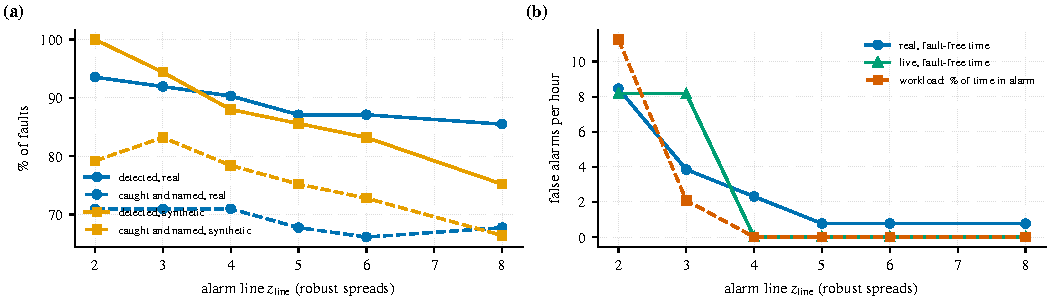
\includegraphics[width=0.98\textwidth]{fig_zline.pdf}
\caption{Sensitivity of the load-aware model to its alarm line (alarm at level 2, that is at twice the line).}
\end{figure}

\subsection{The training window}
\begin{center}
\small
\begin{tabular}{rcccc}
\toprule
Window & Real FA/h & Live FA/h & Organic (FA / alarm) & Steps (FA / alarm)\\
\midrule
60 & 1.5 & 8.2 & 10.4 / 9\% & 7.7 / 6\%\\
\textbf{120} & 2.3 & 0.0 & 0.0 / 0\% & 1.0 / 0\%\\
240 & 1.5 & 0.0 & 0.0 / 0\% & 1.9 / 0\%\\
\bottomrule
\end{tabular}
\end{center}
\begin{simplebox}
Too short a window (60 readings, five minutes) does not hold enough of the signal's natural wobble, so the spread is underestimated and the workload recordings become noisy again. 120 is enough; 240 does not help.
\end{simplebox}

\subsection{The slow reference length}
\begin{simplebox}
120, 360 and 720 readings (10, 30 and 60 minutes) all give essentially the same result (only 120 raised 1.2 false episodes per hour on the organic recording). It matters little once it is long enough; we kept 30 minutes.
\end{simplebox}

\subsection{The drift time for mild shifts}
\begin{center}
\small
\begin{tabular}{rcccc}
\toprule
Readings & Real FA/h & Real alarm time & Synth. detected & Synth. C+N\\
\midrule
\textbf{24 (2 min)} & 2.3 & 6\% & 88\% & 78\%\\
48 (4 min) & 3.1 & 13\% & 89\% & 78\%\\
72 (6 min) & 3.1 & 13\% & 90\% & 78\%\\
120 (10 min) & 3.1 & 13\% & 90\% & 78\%\\
240 (20 min) & 3.1 & 13\% & 90\% & 78\%\\
\bottomrule
\end{tabular}
\end{center}
\begin{simplebox}
We wanted to make the model alarm for longer on mild faults, so we tried longer drift times. It changed nothing on accuracy (caught-and-named stayed at 71\% real, 78\% synthetic) and nothing on the workload recordings, but \emph{doubled} the time in alarm on the real systems (6\% to 13\%) and raised false alarms from 2.3 to 3.1 per hour, because a service whose footprint changes after a restart stays in alarm until accepted. So we kept two minutes and documented the consequence.
\end{simplebox}

\subsection{The range guard (rejected)}
\begin{center}
\small
\begin{tabular}{rcc}
\toprule
Range guard $k$ floors beyond the window range & Steps FA/h & Steps alarm time\\
\midrule
\textbf{off (0)} & 1.0 & 0\%\\
4 & 4.8 & 1\%\\
6 & 2.9 & 0\%\\
10 & 1.0 & 0\%\\
\bottomrule
\end{tabular}
\end{center}
\begin{simplebox}
The old engine had a range guard (``a value far outside what you have seen counts as level 1''). We tried carrying it over to the new model. It changed no result on any fault set and \emph{added} false alarms on the steady-load steps (4.8 per hour at $k=4$ against 1.0 without it). So the new model has none: the robust spread, with its tail-aware part, already scales to the jump.
\end{simplebox}

\subsection{The spread: MAD against tail-aware}
\begin{center}
\small
\begin{tabular}{lcccc}
\toprule
 & Real FA/h & Live FA/h & Organic alarm & Steps alarm\\
\midrule
Load factor, MAD spread & 3.8 & 16.3 & 10\% & 6\%\\
\textbf{Load factor, tail spread} & 2.3 & 0.0 & 0\% & 0\%\\
Control chart, MAD spread & 10.0 & 24.5 & 13\% & 31\%\\
Control chart, tail spread & 2.3 & 0.0 & 0\% & 0\%\\
\bottomrule
\end{tabular}
\end{center}
\begin{simplebox}
The tail-aware spread is the second-biggest improvement after dropping the forest. With the MAD alone, bursty signals look far more extreme than they are, and even the load factor alarms 10\% and 6\% of calm time. With the tail spread both are 0\%.
\end{simplebox}

\section{The ablation of the final model, explained}
\begin{center}
\small
\begin{tabular}{lcccc}
\toprule
 & \multicolumn{2}{c}{Real} & \multicolumn{2}{c}{Synthetic held-out}\\
Variant & C+N & Alarm time & C+N & Alarm time\\
\midrule
Full model & 71 & 6\% & 75 & 4\%\\
$-$ \code{docker stop} fact & 53 & 6\% & 60 & 4\%\\
$-$ crash-loop fact & 71 & 6\% & 68 & 4\%\\
$-$ load factor & 71 & 6\% & 75 & 4\%\\
$-$ tail-aware spread & 71 & 12\% & 75 & 5\%\\
$-$ random walk & 68 & 6\% & 73 & 4\%\\
$-$ one-sided features & 69 & 24\% & 75 & 0\%\\
$-$ two-speed drift & 71 & 13\% & 74 & 14\%\\
Alarm at level 1 instead of 2 & 73 & 12\% & 77 & 7\%\\
\bottomrule
\end{tabular}
\end{center}
\begin{simplebox}
Read the table by columns. \textbf{C+N column:} only the \code{docker stop} fact (53 against 71) and the crash-loop fact (68 against 75 on synthetic) change how many faults are caught and named, plus the walk by a few points. \textbf{Alarm-time column:} the statistical mechanisms (tail spread, one-sided features, two-speed drift) are what keep the model quiet: without one-sided features alarm time on the real systems goes from 6\% to 24\%. The load factor does not change either column on \emph{injected} faults, because the load does not move in them; its value shows only on the workload recordings (Part~\ref{ch:mlstory}).
\end{simplebox}

\begin{saybox}
``Different mechanisms earn their keep on different measures: the facts decide how many faults we catch and name, and the statistical machinery decides whether we stay quiet. The load factor is invisible on injected faults and decisive on workload changes, and that is exactly why we also measured workload changes.''
\end{saybox}

\section{ML question bank}
Extra questions that go deeper than Part~\ref{ch:qa}.

\q{Walk me through what happens to one reading, from raw numbers to an alarm.}\\
\textbf{Answer:} Eight raw numbers are log-transformed (with units) into a vector. The load model compares each signal with the service's slow reference, takes the median shift over busy services as $L$, estimates slopes by ridge, and judges each signal against the service's accepted-window baseline after subtracting $bL$, under two hypotheses, keeping the smaller deviation. The max over signals divided by 4 is the level. If the level holds two readings, it becomes an anomaly (0 below level 0.5, 1 at level 2) and enters the random walk; facts count as level 10. The Hybrid alarms if a fact holds, or the largest level reaches 2, or the rule score reaches 1.25 times its line.

\q{Why log-transform?}\\
\textbf{Answer:} Workload changes are multiplicative, so on a log scale ``twice as busy'' is the same step for a service at 10 requests and one at 10\,000, which lets one load factor describe all services. The unit inside the log stops tiny flows on idle services from turning into big jumps.

\q{Why is the load factor a median and not a regression across services?}\\
\textbf{Answer:} A median is robust: a fault that distorts one or two services cannot move it, so it measures the shared change even while a fault is present. A regression would be pulled by the faulty service.

\q{What if only one service carries traffic?}\\
\textbf{Answer:} Then the load factor is not computed (it needs at least two contributing services) and stays 0. The model then behaves like the control chart.

\q{What if the whole project is faulty, for example the host runs out of memory?}\\
\textbf{Answer:} Then ``everyone moved together'' can look like load. But memory and throttling have slope prior 0, so they are not explained by load; the model only subtracts load from signals that follow it. Container facts (restarts, OOM exits) also raise the alarm directly.

\q{Why two hypotheses instead of just using the learned slope?}\\
\textbf{Answer:} The slope is estimated for a signal across the project; an individual service might ignore the load (a message bus) or follow it (a gateway). Trying both and keeping the smaller deviation handles both before either has been seen to move, and with the load unchanged both agree.

\q{Doesn't taking the minimum over hypotheses hide real faults?}\\
\textbf{Answer:} It can, if a fault happens to look like a load-following move. The risk is largest for a fault that begins during a very large load change. That is stated in the limitations, and the facts and the rules (which do not use the load factor) are a second line.

\q{How does the model avoid learning a fault?}\\
\textbf{Answer:} Only readings under level 1 join the window. A mild shift becomes normal after 24 readings, a large one after 360. So a mild fault is absorbed after two minutes; the rules and facts keep alarming.

\q{Why not just retrain the forest more often?}\\
\textbf{Answer:} A forest of the readings can never explain a workload change, however fresh it is: after a change it would still be in alarm until the window refills, then the window contains the new workload. The problem is not staleness; it is that the model has no notion of load.

\q{Is a deeper neural model a better fix?}\\
\textbf{Answer:} It could learn load dependence if given enough labelled variety, but that needs training data and is not auditable. Our fix is one extra estimate (the median shift) and a subtraction.

\q{How do you know the load factor works rather than just the tail spread?}\\
\textbf{Answer:} Two comparisons. With the tail spread, the control chart already has 0\% time in alarm but still 1.2 and 1.9 false episodes per hour on the two workload recordings; adding the load factor gives 0.0 and 1.0. With the MAD spread, the control chart is in alarm 31\% of the stepped-load recording and the version with the load factor 6\%, so the load factor removes most of the load-driven alarms even when the spread is poor. The tail spread is the larger part of the improvement; the load factor removes what remains.

\q{What is the ridge for, if the slope came out at the prior anyway?}\\
\textbf{Answer:} In our toy case and in much of the data, the load varies little and the prior (slope 1) is right. The ridge prevents wild slopes when the load has barely varied, and lets the slope adapt when it has.

\q{Why is memory not load-following?}\\
\textbf{Answer:} Memory in these services is dominated by fixed footprints, caches and leaks, not by instantaneous traffic; a prior slope of 0 means memory growth is never explained away by load, which is right for leaks.

\q{Why are errors and latency judged only upward?}\\
\textbf{Answer:} Lower error or latency than usual is never a fault of the service, and it follows every restart. Counting it would raise false alarms.

\q{Why do you ignore errors and latency below five requests?}\\
\textbf{Answer:} An error share computed from fewer than five requests is meaningless (one failure out of two is 50\%). So those two signals are treated as missing in that interval.

\q{Why is the first judgement delayed to 30 readings?}\\
\textbf{Answer:} A baseline and a spread need data. Below 30 readings (two and a half minutes) the median and MAD are too uncertain. Until then the service is \emph{not ready} and only container facts apply.

\q{What does ``accepted'' mean on a reading?}\\
\textbf{Answer:} That it was allowed into the training window: it was normal (level under 1), or it was a mild deviation that has lasted 24 readings, or a large one that has lasted 360.

\q{How is the old model's cost spike explained?}\\
\textbf{Answer:} Each service retrains its forests every ten accepted readings. With many services their schedules coincide, so the cost shows 95th-percentile windows nine times the mean. The new model refreshes baselines every four readings, with a peak about three times the mean.

\q{If the load-aware model is not more accurate, why replace the forest?}\\
\textbf{Answer:} Because accuracy on injected faults was never the defect. The defect was a false alarm on every service at every workload change, which the forest cannot fix and the load model does. We also cut the cost by 2.5 times at 320 services.

\q{Why not use the subspace model, which has the best live C+N?}\\
\textbf{Answer:} It is as good at discriminating but raised 7.7--10.7 false episodes per hour on steady load steps, adapts slowly, and costs more as services grow. The load factor was quieter and cheaper. If a project had few services and a strongly shared load, the subspace model would be a reasonable alternative.

\q{Did you test the ML on a system it had never seen?}\\
\textbf{Answer:} On 16 random synthetic topologies scored once, yes. On real systems, we only have our two benches, and the settings were not tuned on a held-out real system; we say the real numbers are optimistic by an unmeasured margin.

\q{What is the single weakest assumption of the load model?}\\
\textbf{Answer:} That the shared workload is a single scalar that all busy services follow with a common slope. If different services follow different parts of the traffic (for example batch jobs and user traffic), a single factor is too crude. The two-hypothesis test softens this, and a multi-factor model is future work.

\chapter{Finding the root cause}
\label{ch:rank}

\section{Step one: split a service's trouble into ``mine'' and ``inherited''}
\begin{simplebox}
Back to the restaurant. The waiter is unhappy because the kitchen is slow. The waiter's unhappiness is real, but it is \emph{explained by the kitchen}. If you ask ``whose fault is it?'' you do not want to point at the waiter.

For each service we ask: is its trouble coming from its \emph{own} resources (its CPU is maxed out, its memory is full), or is it showing only \emph{symptoms} (slow responses, errors, odd traffic) that could simply be inherited from something it calls? CPU, memory and throttling are \emph{own} signals, because a dependency cannot make your CPU spin. Traffic, errors, latency and network are \emph{symptoms}, because you can inherit them. If a service's symptoms are fully explained by a sick service it depends on, we subtract that explanation. What is left is the service's own contribution.
\end{simplebox}

\begin{techbox}
With own level $o(s)$, symptom level $\sigma(s)$ and callees $C(s)$,
\begin{align*}
x(s)&=\gamma\max_{c\in C(s)}a(c),\\
\operatorname{raw}(s)&=\max\bigl(o(s),\ \max(0,\ \sigma(s)-x(s))\bigr),
\end{align*}
where $a(c)$ is the anomaly level of a callee and $\gamma=1.0$ is the weight of what a sick callee explains. A service whose symptoms a sick callee fully explains drops out; one that is abnormal in its own resources stays. The ML engine keeps the two levels (own and symptom) separate for exactly this purpose.
\end{techbox}

\begin{examplebox}[Worked example: three services in a chain]
\code{checkout}\,$\to$\,\code{orders}\,$\to$\,\code{orders-db}. The database's disk is the real problem. Levels right now (1.0 = the service's own alarm line):

\medskip
\begin{center}
\small
\begin{tabular}{lrrr}
\toprule
Service & own level $o$ & symptom level $\sigma$ & what its callee explains $x$\\
\midrule
orders-db & 2.5 & 0.5 & (none, it has no callee) \\
orders & 0.1 & 2.2 & $1.0\times\max(a_{\text{orders-db}})\approx 2.5$\\
checkout & 0.0 & 1.8 & $1.0\times\max(a_{\text{orders}})\approx 2.2$\\
\bottomrule
\end{tabular}
\end{center}

Then $\operatorname{raw}(\text{orders-db})=\max(2.5,\ \max(0,0.5-0))=2.5$. For \code{orders}: $\max(0.1,\ \max(0,2.2-2.5))=0.1$. For \code{checkout}: $\max(0.0,\ \max(0,1.8-2.2))=0.0$. Even though \code{orders} and \code{checkout} are loud (symptoms 2.2 and 1.8), their trouble is explained by the service they call, so they drop to nearly zero. \code{orders-db} keeps 2.5. It is ranked first.
\end{examplebox}

\section{Step two: the random walk}
\begin{simplebox}
The first step is local: it looks at each service and its neighbours. The second step looks at the \emph{whole map}. Imagine a little walker standing on the map. At each step it moves along a link, but it prefers to move toward services that look abnormal and it likes to stay on a service whose trouble nothing downstream explains. Now let the walker walk for a very long time and count how much time it spent at each service. The service it visits the most is the best candidate for the origin. Why? Trouble flows \emph{toward} callers, so the walker following the trail of trouble ends up circling the place it started from.

This idea is a classic (it is the same maths as Google's original PageRank, adapted to a call graph). We did not invent it. We feed it better inputs.
\end{simplebox}

\begin{techbox}
The ranker is a personalised-PageRank walk in the MonitorRank form. A walker on the directed graph steps to a callee $v$ with weight $w(u\to v)\,a(v)$, back to a caller with weight $\rho_{\mathrm b}\,a(u)$, and stays with weight $\max(0,\ a(u)-\max_c a(c),\ o(u))$, restarting on the anomalous set with probability $\alpha=0.15$. The stationary share $\pi_s$ is the score, and services with a container fact rank first. The \emph{stay} term is what lets the true source, whose trouble nothing downstream explains, collect the most mass. The edge weights $w(e)$ are the evidence-weighted confidences of Part~\ref{ch:graph}.
\end{techbox}

\begin{saybox}
``The decomposition removes inherited trouble locally; the random walk then combines that over the whole graph. And facts rank first, because a stopped container is a certainty.''
\end{saybox}

\section{What the evidence says about ranking}
\begin{center}
\small
\begin{tabular}{lcccc}
\toprule
Ranking method (real systems, 62 faults) & C+N & 95\% CI & A@1 & A@3\\
\midrule
Rules & 63 & [52, 74] & 70 & 91\\
Severity (loudest service) & 68 & [56, 79] & 75 & 86\\
ML (load model + walk) & 71 & [60, 81] & 79 & 89\\
Hybrid (default) & 71 & [60, 81] & 79 & 89\\
\bottomrule
\end{tabular}
\end{center}

\begin{simplebox}
\textbf{A@1} is: among the faults we detected, how often was the true root cause ranked first? \textbf{A@3} is: how often was it in the top three? \textbf{C+N} is: out of \emph{all} faults, how often did we detect it \emph{and} rank it first? The bracket is the range in which the true rate probably lies (a 95\% confidence interval).

The interesting part is that the walk is \emph{not} significantly better than just ranking by the loudest anomaly. The difference between Hybrid and Rules is $+8.1$ points with an interval of $[-1.6,+17.7]$ and $p=0.117$. We report this honestly.
\end{simplebox}

\subsection{When does the graph matter? The amplification study}
\begin{simplebox}
In most of our faults the broken service is also the loudest service, so a naive ``loudest first'' wins. That tells you nothing about the graph. To test the case where the graph \emph{should} matter, we made a version where victims get louder than the origin (like a retry storm). We turned up the ``amplification'' knob from 1 (normal) to 4 (victims feel it four times as hard). If the graph logic is worth anything, ranking by the walk should hold up while ranking by loudness should fall.
\end{simplebox}

\begin{figure}[H]
\centering
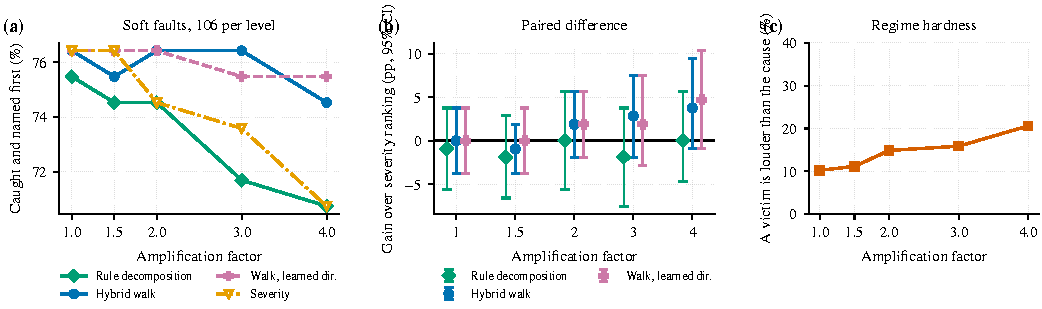
\includegraphics[width=0.98\textwidth]{fig_amp.pdf}
\caption{Amplification study on soft faults (106 per level).}
\end{figure}

\begin{techbox}
Soft faults (brownout, latency, memory) were regenerated with the amplification factor $A\in\{1,1.5,2,3,4\}$, the hybrid's alarms were kept identical for every ranker and only the ranking varied. As $A$ grows, the share of faults in which some victim is louder than the true cause rises from 10\% to 21\%, the severity ranking falls from 76\% to 71\%, and the walk holds at 75--76\%, so the gain of the walk over severity grows from zero to $+3.8$ points (95\% CI $[-0.9,+9.4]$ at $A=4$) and that of the walk with learned directions to $+4.7$ ($[-0.9,+10.4]$). The intervals include zero at every level. So the shape is as the theory predicts, but the sample is too small to confirm it.
\end{techbox}

\begin{warnbox}
Do not claim ``the graph ranking is proven better''. Say ``it behaves as theory predicts as amplification grows, the gain is a few points, and our sample is too small to confirm it''.
\end{warnbox}

\section{Per-class accuracy: where it works and where it does not}
\begin{figure}[H]
\centering
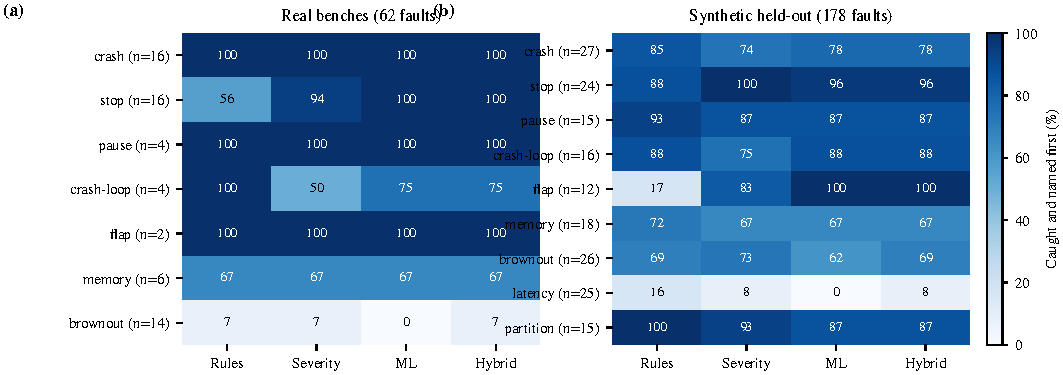
\includegraphics[width=0.98\textwidth]{fig_class.pdf}
\caption{Caught-and-named rate by fault class (percent; $n$ faults per class), on the real systems (a) and the synthetic held-out set (b).}
\end{figure}

\begin{simplebox}
The tool is best at faults with a clear \emph{fact} (a container that stops or is paused) and weakest at \emph{brownouts}: a service that is slowed down by a resource limit but not stopped, especially when it was nearly idle to begin with. A nearly idle service that gets slower barely changes any of the eight numbers, so there is nothing for any detector to see. That is an honest open problem; we show it on the figure and say it in the limitations.
\end{simplebox}

\chapter{Predicting who is next: the cascade model}
\label{ch:cascade}

\section{The idea}
\begin{simplebox}
Once a service is in trouble, the interesting question for the engineer is: \emph{who else is about to be hurt?} Not every dependency passes trouble along. A service with a timeout, a cache or a circuit breaker may shrug off a failing dependency. A service with none of those may collapse right away. We cannot read the code to find out which is which, so we \emph{learn it from experience}: every time one service goes bad, we look at the services that call it and ask, within a minute, did they go bad too? Over time each connection collects a track record, like ``this link has passed trouble along 6 times out of 8''.
\end{simplebox}

\begin{techbox}
Each call edge $c\to x$ carries an unknown probability $p(c\leftarrow x)$ that trouble in $x$ reaches its caller $c$. Whenever a service $x$ turns abnormal, every healthy caller $c$ is one \emph{trial}; it succeeds if $c$ turns abnormal within one minute (12 windows). With $k$ successes in $n$ trials and a Beta prior of mean $\pi_0$ and strength $m$, the posterior mean is
\[
\hat p(c\leftarrow x)=\frac{k+m\,\pi_0}{n+m}.
\]
All experiments use an uninformative prior ($\pi_0=0.5$, $m=2$). No labels are needed: the trials are the system's own history.
\end{techbox}

\begin{examplebox}[Worked example: one edge's track record]
Prior: mean $0.5$, strength $2$ (so it behaves like having seen 1 success and 1 failure). The edge \code{orders}$\leftarrow$\code{orders-db}.

\begin{center}
\small
\begin{tabular}{lcc}
\toprule
After & $k/n$ & $\hat p=(k+1)/(n+2)$\\
\midrule
no trials & 0/0 & $1/2=0.50$\\
1 trial, success & 1/1 & $2/3=0.67$\\
3 trials, 3 successes & 3/3 & $4/5=0.80$\\
8 trials, 6 successes & 6/8 & $7/10=0.70$\\
8 trials, 1 success & 1/8 & $2/10=0.20$\\
\bottomrule
\end{tabular}
\end{center}

A rarely used edge stays close to $0.5$ (the prior) and moves as evidence arrives. An edge that has repeatedly failed to pass trouble drifts down. This is the standard Bayesian update for a rate, and it is simple enough to do by hand in a viva.
\end{examplebox}

\section{From edge probabilities to ``risk of a service''}
\begin{simplebox}
Suppose we suspect the database is the origin. A service two steps away can be hit by two different routes. Each route is a chain of ``trouble crosses this link'' events, so the chance along a route is the \emph{product} of the link chances. Then, if there are two independent routes, the service is hit if \emph{either} route delivers it. The chance that neither does is the product of the two failures, so the chance of being hit is one minus that. This rule is called \emph{noisy-OR}.
\end{simplebox}

\begin{techbox}
Given a suspected root $r$, risk flows up the call graph by noisy-OR, the independent-cascade model of influence spread:
\[
P(r)=1,\qquad P(c)=1-\prod_{x\in C(c)}\bigl(1-P(x)\,\hat p(c\leftarrow x)\bigr).
\]
Services already abnormal are dropped, services above a risk cut are reported as likely next, and $\sum_c P(c)$ estimates the blast radius.
\end{techbox}

\begin{examplebox}[Worked example: the gateway with two routes]
A four-service graph. Root \code{db} is sick ($P=1$). The \code{gateway} calls two services, \code{orders} and \code{catalog}, and both call \code{db}.

Learned edge probabilities: $\hat p(\text{orders}\leftarrow\text{db})=0.8$, $\hat p(\text{catalog}\leftarrow\text{db})=0.4$, $\hat p(\text{gateway}\leftarrow\text{orders})=0.5$, $\hat p(\text{gateway}\leftarrow\text{catalog})=0.5$.

\begin{align*}
P(\text{orders})&=1-(1-1\times0.8)=0.80\\
P(\text{catalog})&=1-(1-1\times0.4)=0.40\\
P(\text{gateway})&=1-(1-0.80\times0.5)(1-0.40\times0.5)\\
&=1-(0.60)(0.80)=1-0.48=0.52.
\end{align*}

So the gateway has about a 52\% chance of being hit via its two routes. If we had used plain reachability (``is there any path?'') the gateway would be marked 100\% affected, which overstates what happens when callers have protections.
\end{examplebox}

\section{How good are the predictions?}
\begin{figure}[H]
\centering
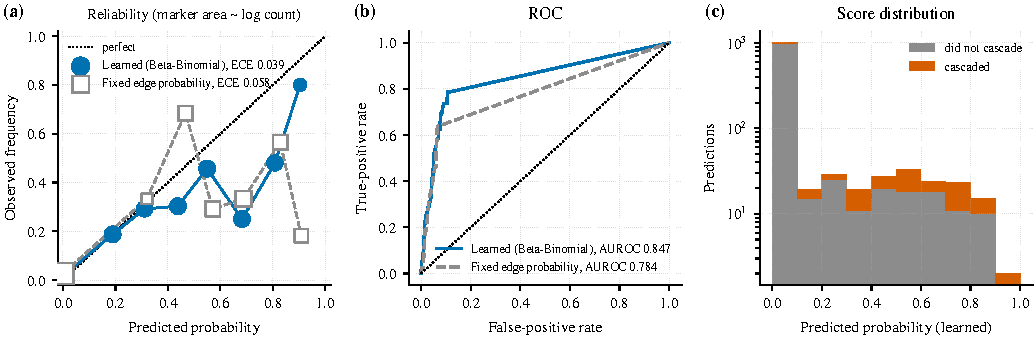
\includegraphics[width=0.98\textwidth]{fig_calibration.pdf}
\caption{Who-is-next prediction on the synthetic held-out set. (a) Reliability diagram. (b) ROC curves. (c) Distribution of the learned probabilities.}
\end{figure}

\begin{simplebox}
A good prediction has two properties. It should \emph{rank} well (the services that really fall are among the highest). And it should be \emph{honest about its numbers} (when it says 70\%, about 70\% of those services really fall). The second property is called \emph{calibration}. Our learned model ranks only slightly better than a fixed-probability version, but it is clearly \emph{better calibrated}: its percentages mean what they say.
\end{simplebox}

\begin{techbox}
On the synthetic held-out set (163 faults, 1\,289 predictions, 69 cascades) the learned propagation model reaches AUROC 0.841 against 0.827 for the same noisy-OR with every edge fixed at 0.7, a Brier score of 0.047 against 0.052 and an expected calibration error of 0.033 against 0.051. The reliability curve is noisy in the upper bins, which hold few predictions. Brier score $=\frac1n\sum_i(p_i-y_i)^2$; ECE $=\sum_b\frac{n_b}{n}\lvert\bar p_b-\bar y_b\rvert$ over equal-width bins.
\end{techbox}

\begin{warnbox}
On the \emph{real} systems this experiment cannot be done well: only 10 of 535 predictions were followed by a cascade, because real faults are mostly single-service outages that the systems absorb. The real-system comparison (AUROC 0.742 against 0.633) is not informative. Never say ``learned cascade prediction works on real systems''. Say ``it is better calibrated on synthetic cascades, and real cascades were too rare for a real-system test''.
\end{warnbox}

\begin{saybox}
``Noisy-OR is the independent-cascade model. Our contribution is learning the edge probabilities online as Beta--Binomial posteriors from the system's own incidents. Calibration is better than fixed probabilities (ECE 0.033 against 0.051); ranking is only slightly better; and on real systems cascades were too rare to test it.''
\end{saybox}

\chapter{Early warning, change points and fault typing}
\label{ch:more}

These three pieces sit on top of the main pipeline. They do \emph{not} change what is detected or how it is ranked (with one exception noted below). They add information for the operator.

\section{Early warning: a trend before the alarm}
\begin{simplebox}
Some faults arrive slowly. A memory leak climbs for ten minutes before the service dies. A normal alarm only fires when the line is crossed. An early warning looks at the \emph{direction} the number is heading. If a service's deviation has been rising steadily over the last two minutes, and the straight line through those points will cross the alarm line within the next two minutes, we flag it early.
\end{simplebox}

\begin{techbox}
For each rising-only feature, a least-squares line fitted to the load-aware residual $z$ over the last two minutes (24 readings) and projected two minutes ahead flags a service that has not reached the alarm level but will. Only lines with $R^2\ge0.6$ count, so a noisy up-down wobble does not trigger a warning.
\end{techbox}

\begin{figure}[H]
\centering
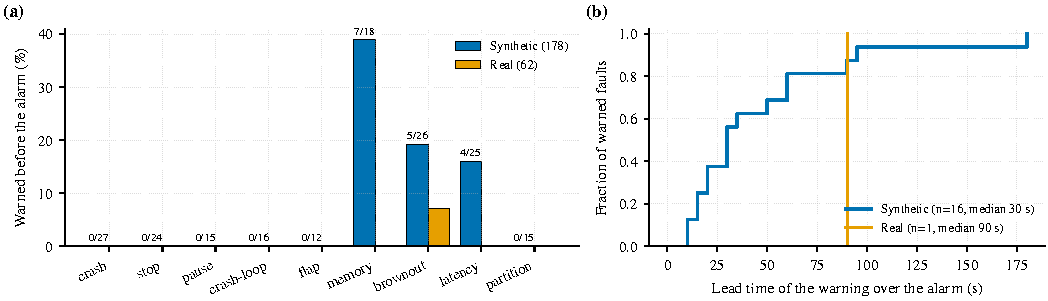
\includegraphics[width=0.98\textwidth]{fig_early.pdf}
\caption{Early warning. (a) Share of faults warned before the alarm, by fault class. (b) Lead time of the warnings over the alarm.}
\end{figure}

\begin{warnbox}
This is the \textbf{weakest} part of the system, and the report says so. On the synthetic set it warns before the alarm for 13 of 178 faults (7 of 18 memory leaks, 4 of 25 latency faults, 2 of 26 brownouts) with a median lead of 25 seconds and 0.8 false warning episodes per fault-free hour. On the real systems it fired before the alarm for \emph{none} of the 62 faults, because those faults are abrupt, and raised 6.9 false warning episodes per hour. If asked ``does it predict failures?'', say ``it warns early for some gradual faults in simulation; on our real, abrupt faults it did not, and we report it as the weakest component''.
\end{warnbox}

\section{Change-point alarms: faster, at a price}
\begin{simplebox}
A usual alarm waits until a number is clearly beyond its normal range. A \emph{change-point} detector instead notices that the \emph{average has shifted}, which can happen a few seconds sooner. It is like noticing that a car has started drifting before it actually leaves the lane. The trade is that it also reacts to harmless shifts, so you spend more time in alarm.
\end{simplebox}

\begin{techbox}
We used online Page--Hinkley change-point detection on the raw metrics as an additional alarm source. On the real systems it lifts the detected fraction from 90\% to 95\% and cuts the median detection delay from 11.3\,s to 4.8\,s, but alarm time rises from 8\% to 16\%. On the synthetic set, whose faults are abrupt, the curves almost coincide. It is available as a research variant; the shipped default does not use it.
\end{techbox}

\begin{figure}[H]
\centering
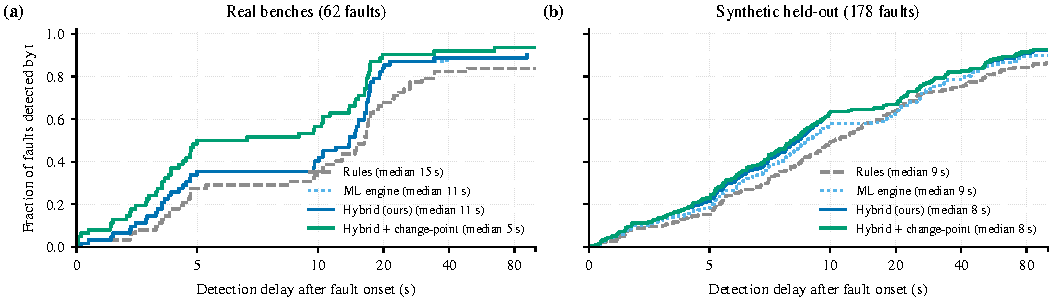
\includegraphics[width=0.98\textwidth]{fig_delay.pdf}
\caption{Detection delay after fault onset as a cumulative distribution.}
\end{figure}

\begin{saybox}
``Change-point alarms cut the median detection delay from 11.3 to 4.8 seconds on the real systems, but they double the time in alarm, from 8 to 16 percent. We list it as a trade-off, not a free win, which is why it is not the default.''
\end{saybox}

\section{Naming the type of fault and attaching a runbook}
\begin{simplebox}
When an alarm fires and we have a top suspect, the engineer's next question is ``what kind of problem is it?'': did it crash, was it stopped on purpose, is it crash-looping, is it leaking memory, is it just slow? We use a small decision-tree-style classifier (a random forest) that looks at 35 things about that service's recent telemetry and names the type. Then we attach a short checklist of two to four concrete commands for that type, like ``check \code{docker logs}'' or ``look at the memory limit''. The classifier only labels and advises. It never changes the alarm or the ranking.
\end{simplebox}

\begin{techbox}
At the alarm, 35 features of the top suspect's telemetry (container-state history, exit code, number of separate outages, memory slope, CPU and throttling change, latency and error ratios against a pre-fault baseline, network drop, number of anomalous callers) go to a random forest that names the fault type: crash, stop, pause, crash-loop, flap, memory, brownout, latency or partition. A runbook of two to four concrete checks per type is attached. With the true service the forest is correct for 99\% of synthetic faults 60\,s after the alarm; on the engine's own suspect it is 79\%, because a wrong suspect is rarely typed correctly. On the real systems a hand-written decision list generalises best (64\% on the suspect, 84\% on the true service), because real flaps are pause cycles and real brownouts on idle services show no throttling --- differences between the simulator and reality that the learned models absorb as synthetic-specific patterns.
\end{techbox}

\begin{figure}[H]
\centering
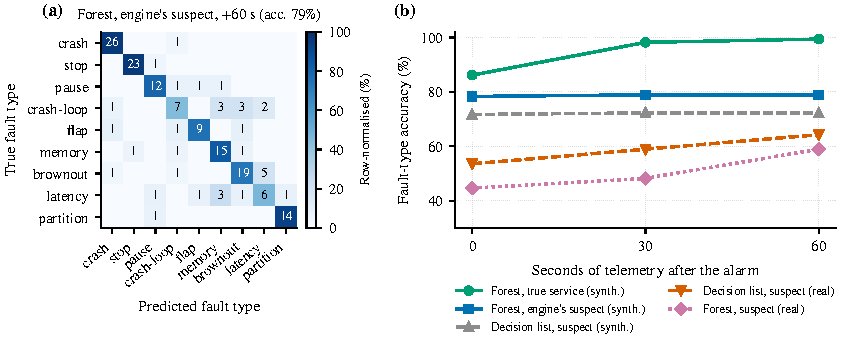
\includegraphics[width=0.78\textwidth]{fig_diag.pdf}
\caption{Fault-type diagnosis. (a) Confusion matrix of the random forest on the engine's suspect 60\,s after the alarm. (b) Accuracy against seconds of telemetry after the alarm.}
\end{figure}

\section{Learned directions: a robustness feature}
\begin{figure}[H]
\centering
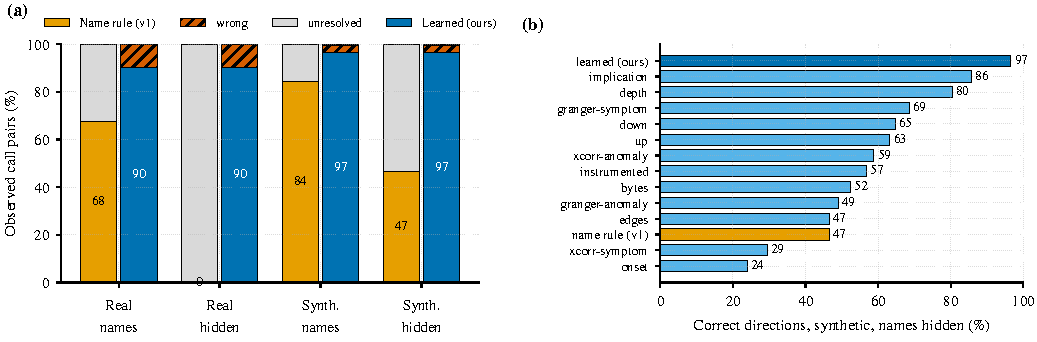
\includegraphics[width=0.98\textwidth]{fig_dirs.pdf}
\caption{Call directions. (a) Share of observed true-call pairs oriented correctly, wrongly or left unresolved, with names shown or hidden. (b) Correct share of each signal with names hidden.}
\end{figure}

\begin{simplebox}
We explained learned directions in Part~\ref{ch:graph}. Here is the result in plain words. When names tell you which service is a database, which is a gateway and so on, the simple name rule gets 21 of 31 pairs right and leaves 10 undecided; the learned rule gets 27 of 31 (4 wrong). When names are hidden (renamed ``alpha, bravo, ...''), the name rule is undecided for every pair and the learned rule is unchanged. On ranking the effect is small: with names available, learned directions are \emph{not} better than the name rule (68\% against 71\%, $-3.2$ points, not significant). With names hidden they reach 68\% against 66\% for the name rule and 71\% for the true graph. So learned directions are a \emph{robustness} mechanism, not an accuracy gain.
\end{simplebox}

\section{Cost: can this run live?}
\begin{figure}[H]
\centering
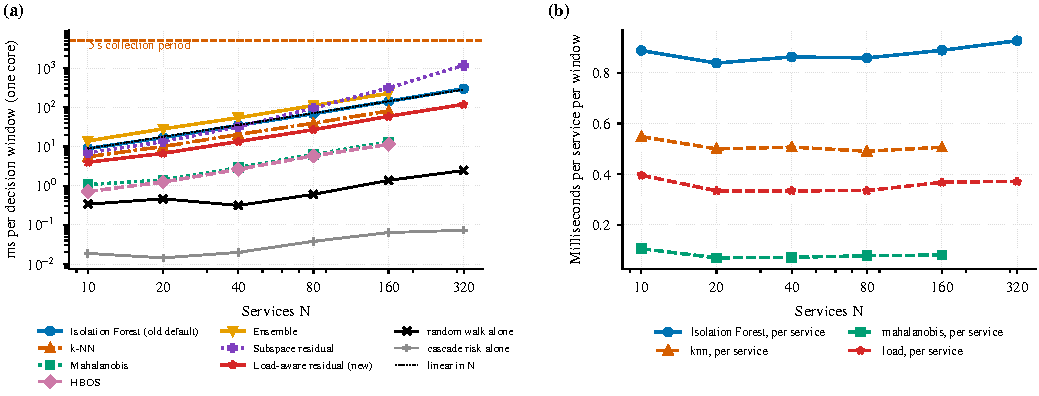
\includegraphics[width=0.98\textwidth]{fig_scale.pdf}
\caption{Cost of one decision window against the number of services (single core, logarithmic axes; the dashed line is the 5\,s collection period).}
\end{figure}

\begin{simplebox}
Does the thinking take long? No. For one service, one decision takes about a third of a millisecond. For ten services about four milliseconds; for 320 services about a tenth of a second. The mapper only needs to finish within five seconds, so it has a lot of room. The cost grows in a straight line with the number of services: twice the services, twice the cost.
\end{simplebox}

\begin{techbox}
The adopted load-aware model costs about $0.37$\,ms per service per window and grows linearly: 4.0\,ms for 10 services, 26.8\,ms for 80 and 119\,ms for 320 (95th percentile 356\,ms), always far below the 5\,s collection period. The old forest cost about $0.9$\,ms per service (296\,ms for 320) with 95th-percentile windows nine times the mean, because every service refits at once every ten readings; the load-aware model refreshes its baselines every four readings with a much smaller peak (about three times the mean). The subspace residual grows faster than linearly (1.2\,s for 320 services, with 11\,s windows at the 95th percentile) because its covariance has one row per service-signal pair. On the two benches (12 and 13 services) a window takes about 5\,ms. These are wall-clock times on one core of a shared four-core virtual machine, not a tuned benchmark.
\end{techbox}

\chapter{The dashboard: a guided tour}
\label{ch:ui}

Use this part to rehearse the demo. For each page: what it shows, what to point at, and one sentence to say.

\section{The sidebar and the top bar}
\begin{simplebox}
On the left there is a menu with the pages. In the top bar you pick a project (or ``All projects''), see how many services are healthy, degraded or critical, and use the \textbf{Rules / Hybrid / ML} switch. At the right there is a green ``Live'' light and the time of the last update. While a project is still learning its normal behaviour the bar says ``Learning baseline, 5 of 30 min''. That is honest: for the first thirty minutes a project has no learned rule model, and only container facts (a stopped container) can raise incidents.
\end{simplebox}

\begin{techbox}
Pages: \emph{Incidents \& cascade}, \emph{Detection engines}, \emph{Cascade risk}, \emph{Spatial view} (3D), \emph{Architecture} (2D), \emph{Telemetry}, \emph{Traces}, \emph{Dependencies}, \emph{Analytics}. Three research pages (ML pipeline, model findings from the optional Python sidecar, experiment history) are hidden until the operator switches them on under ``Show research tools''. The setting \code{MAPPER\_BASELINE\_MIN} (30) controls the learning period.
\end{techbox}

\section{Architecture (2D)}
\begin{figure}[H]
\centering
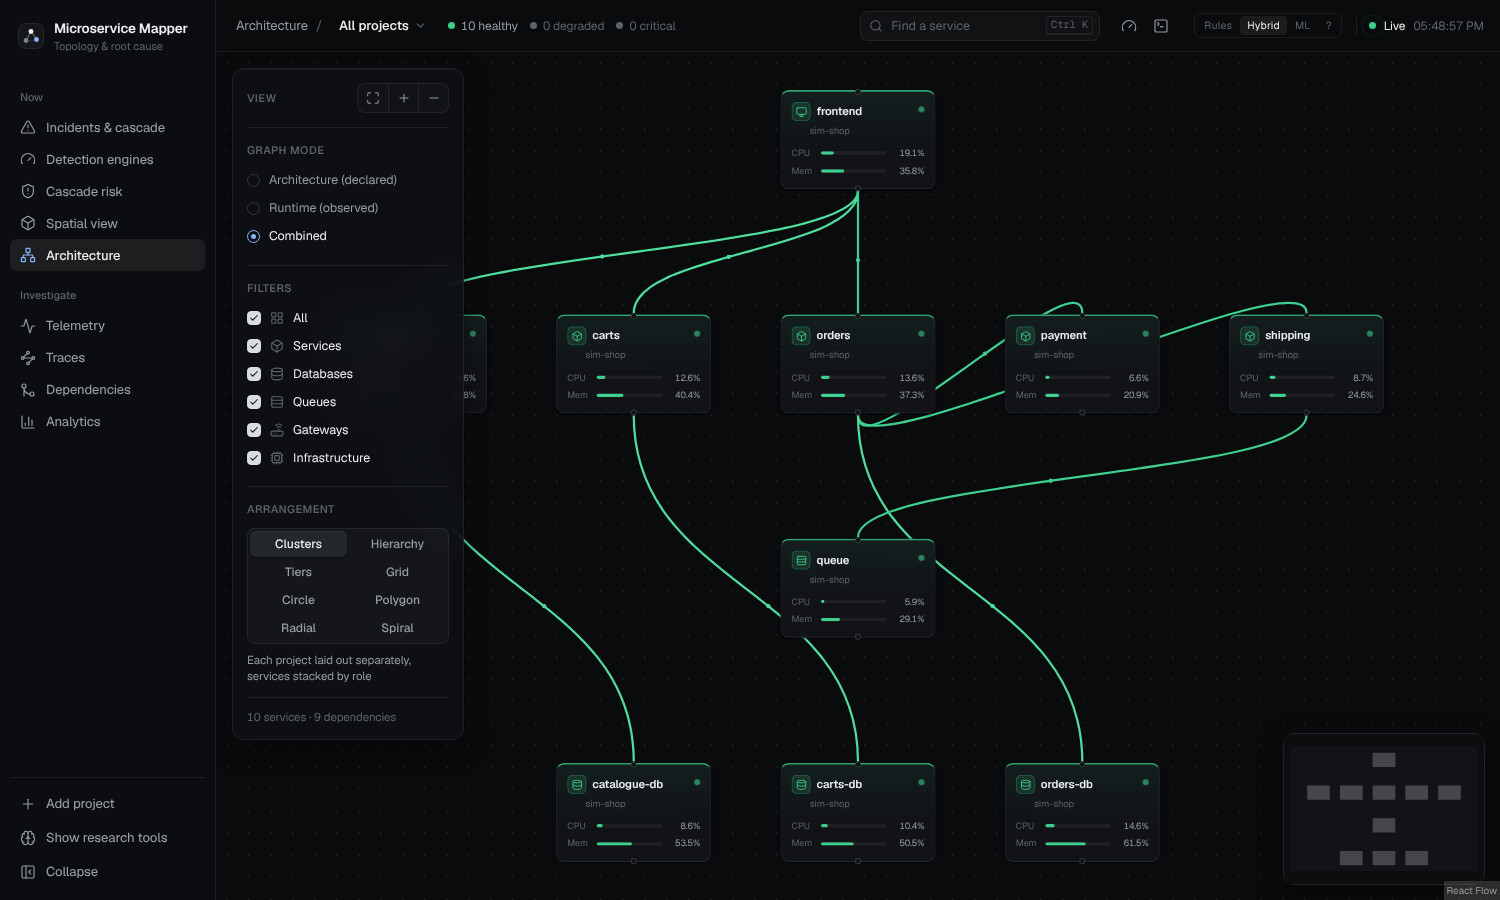
\includegraphics[width=0.96\textwidth]{ui_architecture.jpg}
\caption{The 2D dependency graph with arrangement and filter controls.}
\end{figure}
\begin{simplebox}
The flat map of services as boxes joined by lines. Each box shows CPU and memory against the container's own allowance. Lines show dependencies, and when we have actually seen traffic on them, their activity. You can choose different layouts (clusters, hierarchy, tiers, grid, circle, radial, spiral).
\end{simplebox}
\begin{saybox}
``This is the map the rest of the system works on. Declared and observed links are both shown; observed ones carry evidence.''
\end{saybox}

\section{Incidents and cascade}
\begin{figure}[H]
\centering
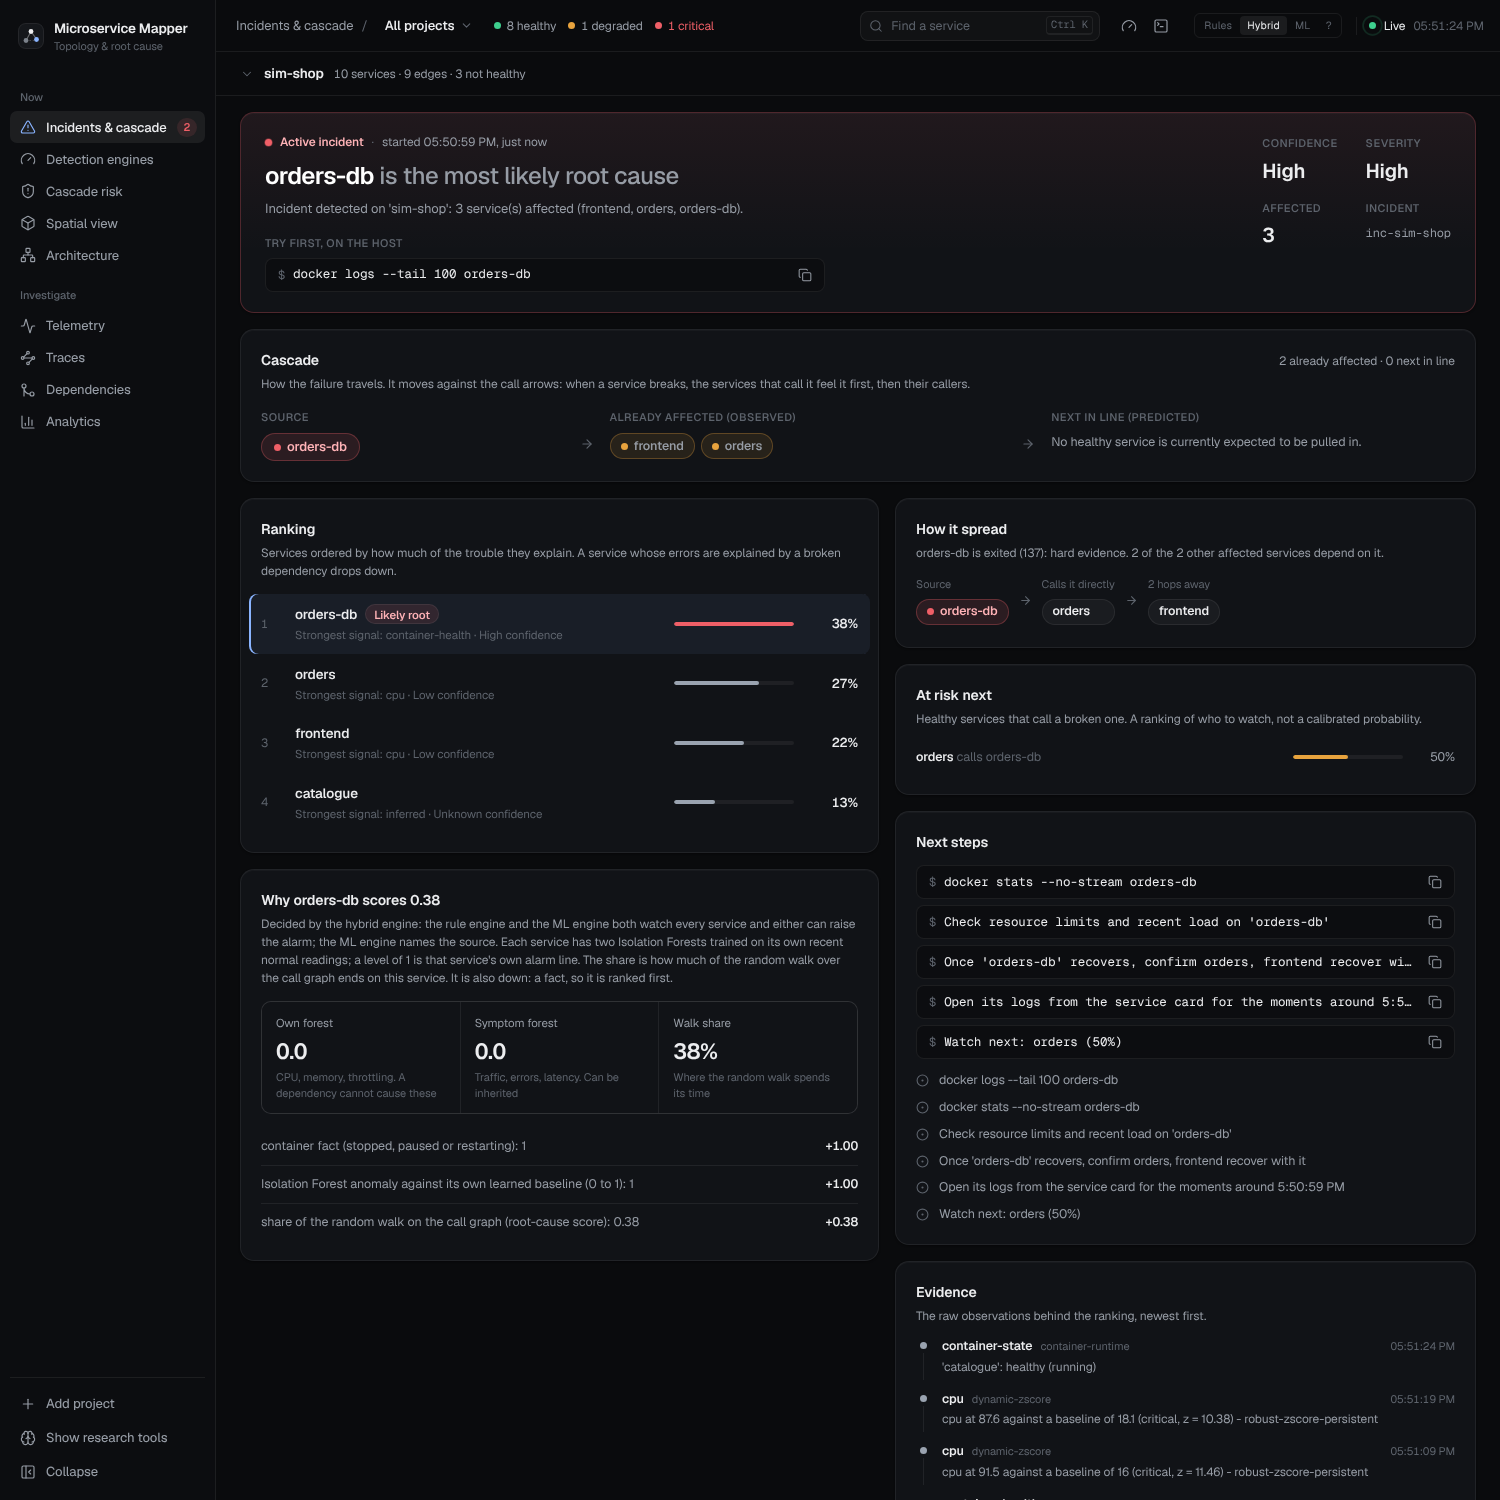
\includegraphics[width=0.78\textwidth]{ui_incident_active.png}
\caption{An active incident after \code{orders-db} was killed.}
\end{figure}
\begin{simplebox}
When something goes wrong, this page opens an incident. At the top: the most likely root cause, how confident the tool is, and how severe. Below that: a \emph{cascade panel} with three groups --- the source, the services already affected, and the services predicted to be next. A \emph{ranking} lists each service with the strongest signal behind its score. A \emph{Why} panel splits a score into its own, symptom and walk parts, and lists the evidence. At the bottom, \emph{next steps}: concrete commands to run on the host.
\end{simplebox}
\begin{saybox}
``Read it top to bottom: who, how sure, who is hurt, who is next, why, and what to do. Every number has a parts breakdown you can open.''
\end{saybox}

\section{Detection engines (the page for the ML story)}
\begin{figure}[H]
\centering
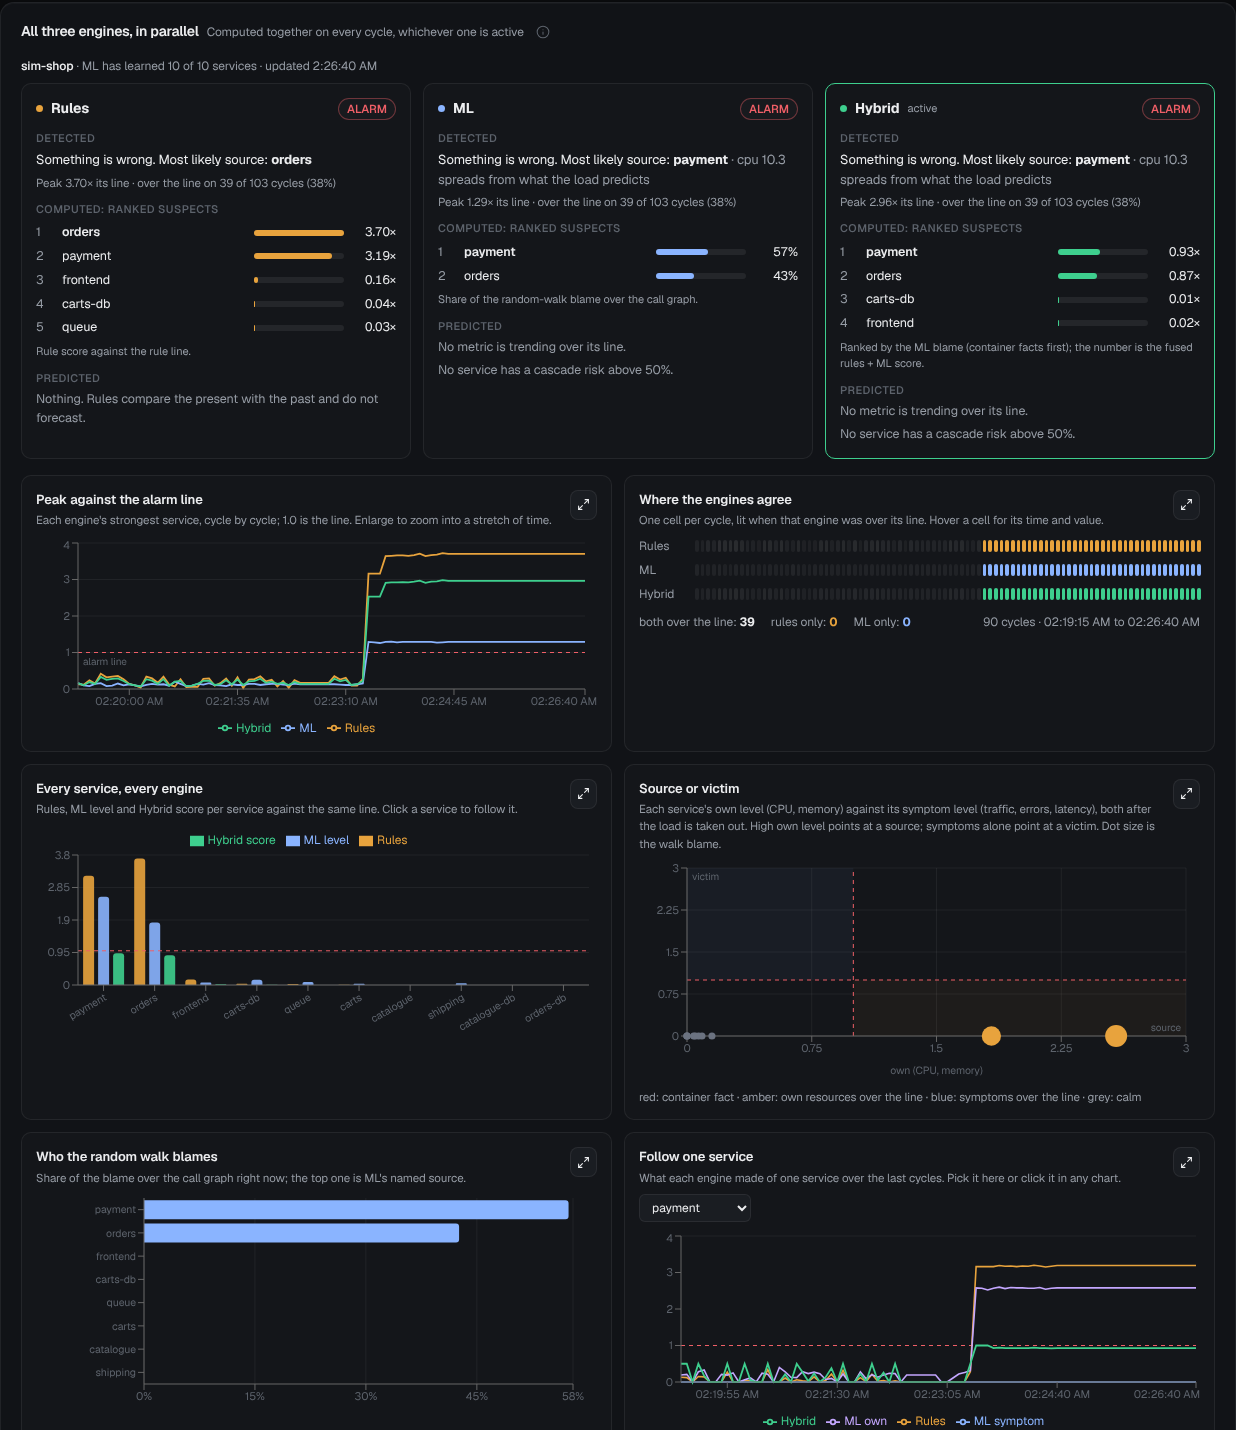
\includegraphics[width=0.92\textwidth,height=0.78\textheight,keepaspectratio]{ui_engines_alarm.png}
\caption{The Detection engines page during a slow-payment fault.}
\end{figure}
\begin{simplebox}
This is the page to use when you explain the ML correction. The top explains Rules, ML and Hybrid in four short lines each. The three middle columns show \emph{what each engine thinks right now about the same data}. In the screenshot, Rules blame \code{orders} (the louder victim); ML and Hybrid name \code{payment} and say \emph{why} (``cpu 10.3 spreads from what the load predicts''). A small chip beside the project name says whether the shared workload moved. Below are six charts; each has a button that enlarges it into a pop-up with a brush for zooming into a few seconds of time.
\end{simplebox}

\begin{techbox}
Charts: each engine's peak against its alarm line; a strip showing the cycles on which the engines agreed; the level of every service under every engine; a source-or-victim scatter (own resources against symptoms); the share of blame from the random walk; a trail for one chosen service. The page ends with the configuration of both engines in plain words (alarm line 4 spreads, alarm level 2, persistence 2 windows, window 120, slow reference 360 readings, and so on).
\end{techbox}

\begin{figure}[H]
\centering
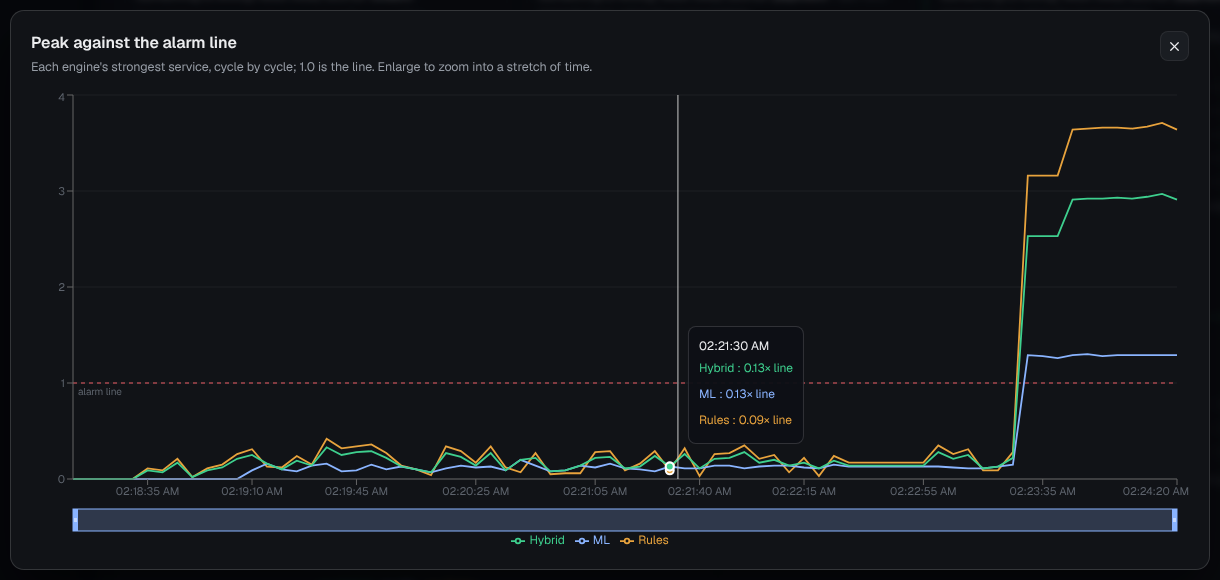
\includegraphics[width=0.9\textwidth]{ui_engines_popup.png}
\caption{An enlarged chart with its time brush and hover read-out.}
\end{figure}

\begin{saybox}
``Look at the pop-up: the rule score climbs higher than the ML peak, but on the wrong service. The ML peak crosses the line once and stays just above it, on the right service. That is the whole difference between the engines, on one chart.''
\end{saybox}

\begin{warnbox}
In the demo on the simulator, the ML engine alarms on the slow \code{payment} fault and then, after about 48 simulated seconds, absorbs it and goes quiet (its two-minute drift rule). The Rules and Hybrid engines keep alarming. If someone asks why ML went quiet, that is the answer, and it is in the limitations.
\end{warnbox}

\section{Cascade risk}
\begin{figure}[H]
\centering
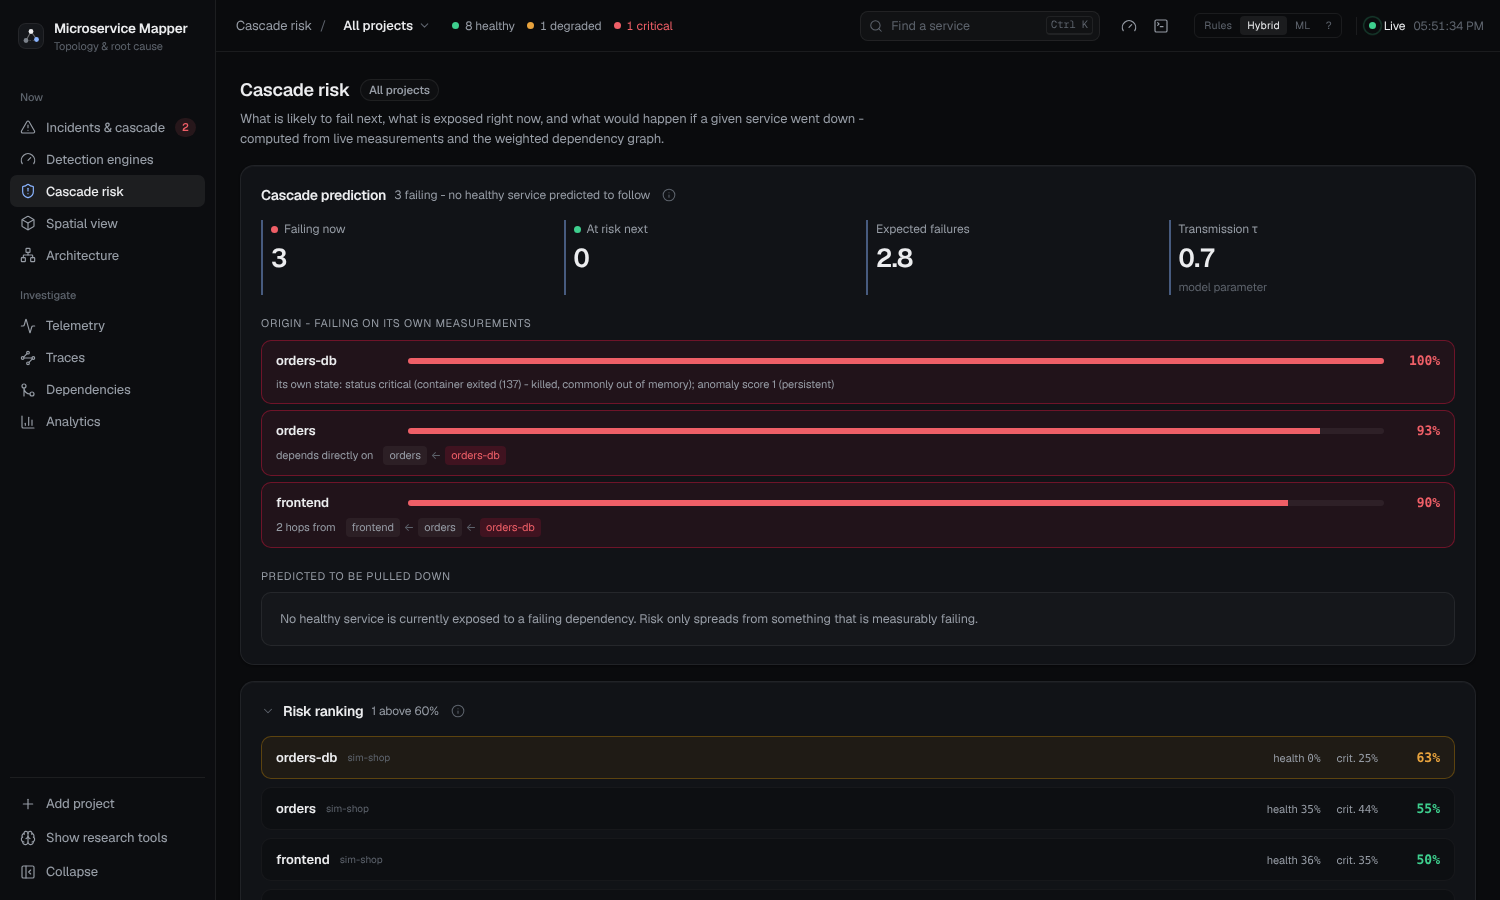
\includegraphics[width=0.96\textwidth]{ui_cascade_risk_fault.png}
\caption{Cascade risk during the fault.}
\end{figure}
\begin{simplebox}
Three questions in one page: what is failing now (judged on its own measurements), what is exposed (which services have a lot depending on them), and what would happen if a chosen service failed (what-if). Every prediction shows the \emph{name of the model and its parameter} beside it. No bare numbers.
\end{simplebox}

\section{Telemetry, Traces, Dependencies, Analytics}
\begin{figure}[H]
\centering
\setlength{\tabcolsep}{2pt}
\begin{tabular}{cc}
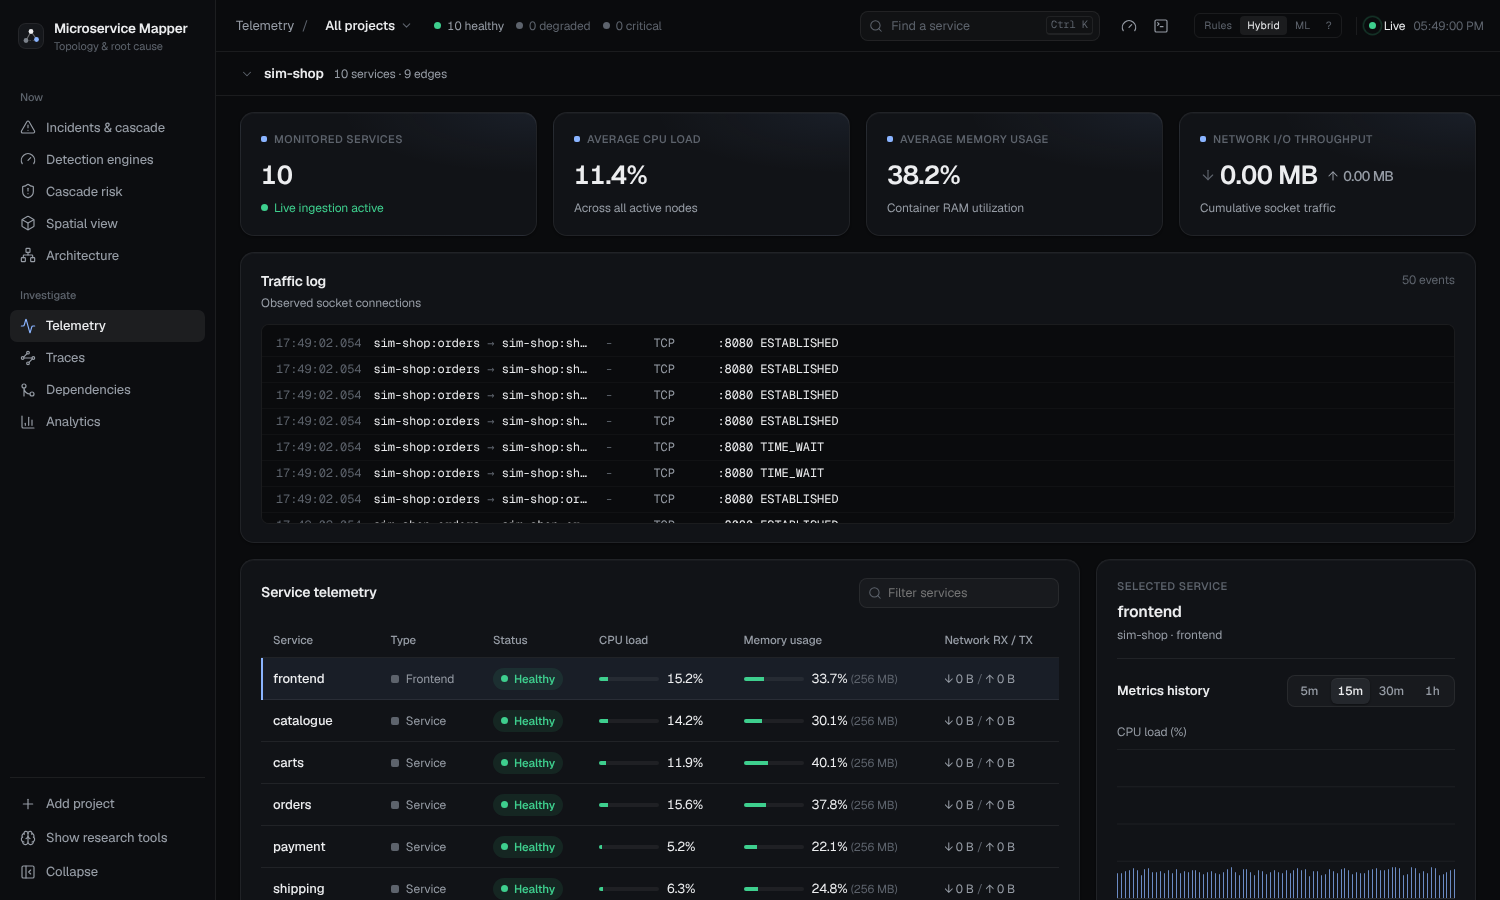
\includegraphics[width=0.49\textwidth]{ui_telemetry.png} & 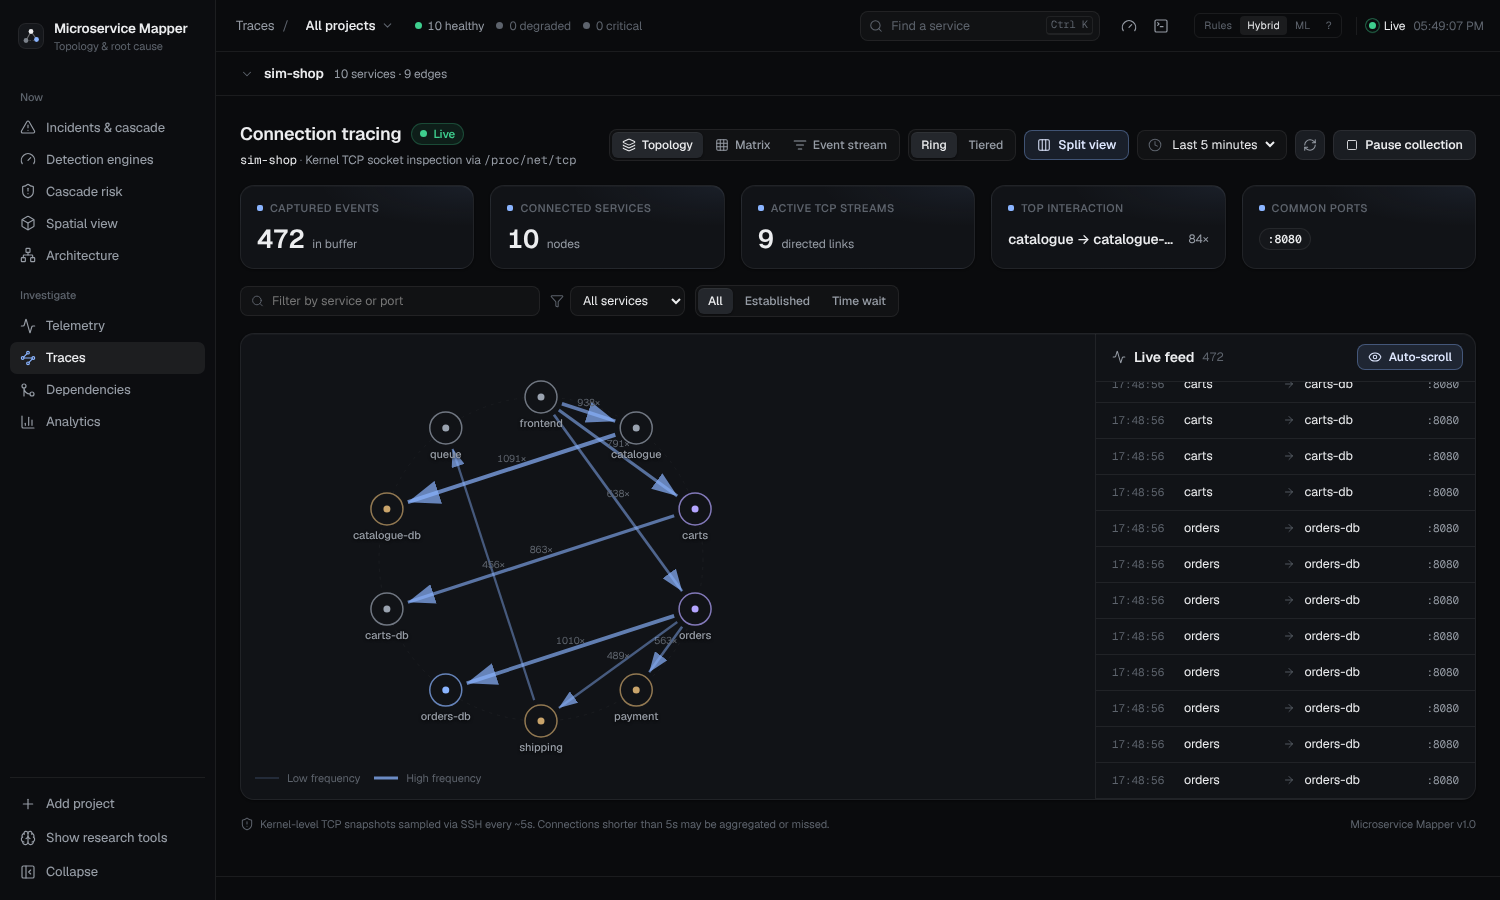
\includegraphics[width=0.49\textwidth]{ui_traces.png}\\
\small (a) Telemetry & \small (b) Traces\\[4pt]
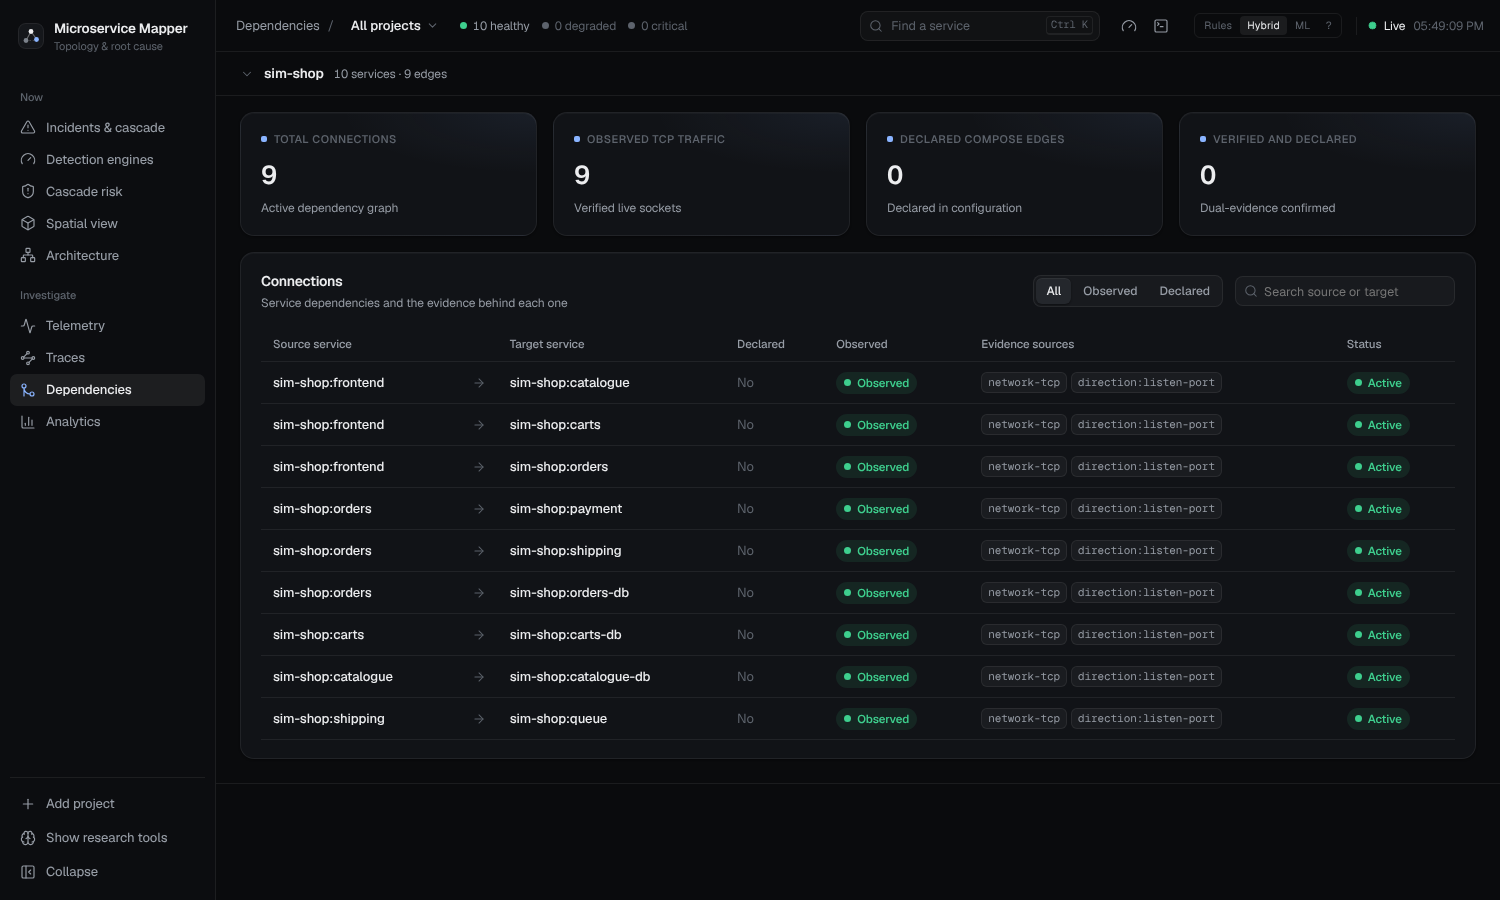
\includegraphics[width=0.49\textwidth]{ui_dependencies.png} & 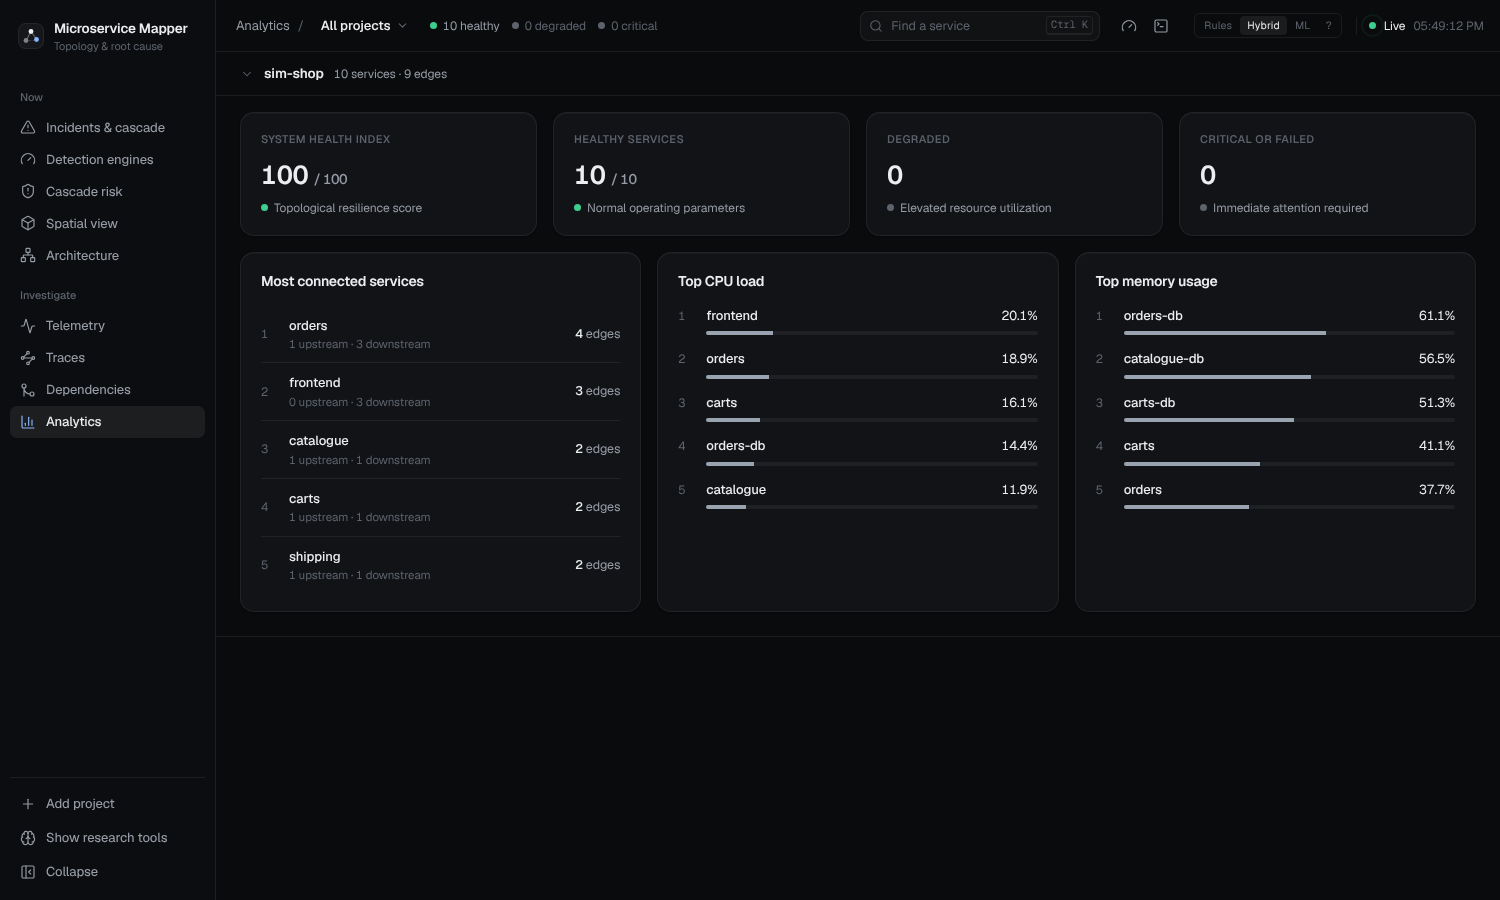
\includegraphics[width=0.49\textwidth]{ui_analytics.png}\\
\small (c) Dependencies & \small (d) Analytics
\end{tabular}
\caption{The investigation pages.}
\end{figure}
\begin{simplebox}
\textbf{Telemetry} is the raw numbers: fleet totals, the live connection log, a sortable per-service table with a history chart. \textbf{Traces} shows sampled connections as a ring, a matrix or an event stream; it is \emph{not} request tracing. \textbf{Dependencies} lists every connection with its declared and observed flags and the evidence sources (for example \emph{network-tcp} and \emph{direction:listen-port}). \textbf{Analytics} gives a health index, the counts of healthy/degraded/critical services, the most connected services and the top CPU and memory users.
\end{simplebox}

\begin{warnbox}
The ``Traces'' page name is a trap. It is not distributed tracing. It is a view of sampled TCP sockets. Say so before an evaluator assumes otherwise.
\end{warnbox}

\section{The 3D spatial view}
\begin{simplebox}
The 3D view draws the same graph as a small city. Services are buildings on platforms. Links are cables: thick cables are heavily used links; the colour shows how healthy the link is; and little pulses move along them faster when the link carries more requests. A card floats over each platform with its role and how many services it holds. A \emph{Cards} button hides the cards when they cover things.

Four arrangements answer four questions:
\begin{itemize}
\item \textbf{Islands}: ``what kinds of services do I have?'' --- one raised platform per role (edge, services, messaging, data).
\item \textbf{Flow}: ``in what order does a request travel?'' --- platforms in order from entry points to data, with a note on how many callers a fault at each hop can reach.
\item \textbf{Topology}: ``what would hurt the most if it broke?'' --- services grouped by how much depends on them.
\item \textbf{Tiers}: ``are my layers respected?'' --- layers stacked as terraces from edge down to data; a call that skips a layer or goes up the stack stands out.
\end{itemize}
\end{simplebox}

\begin{figure}[H]
\centering
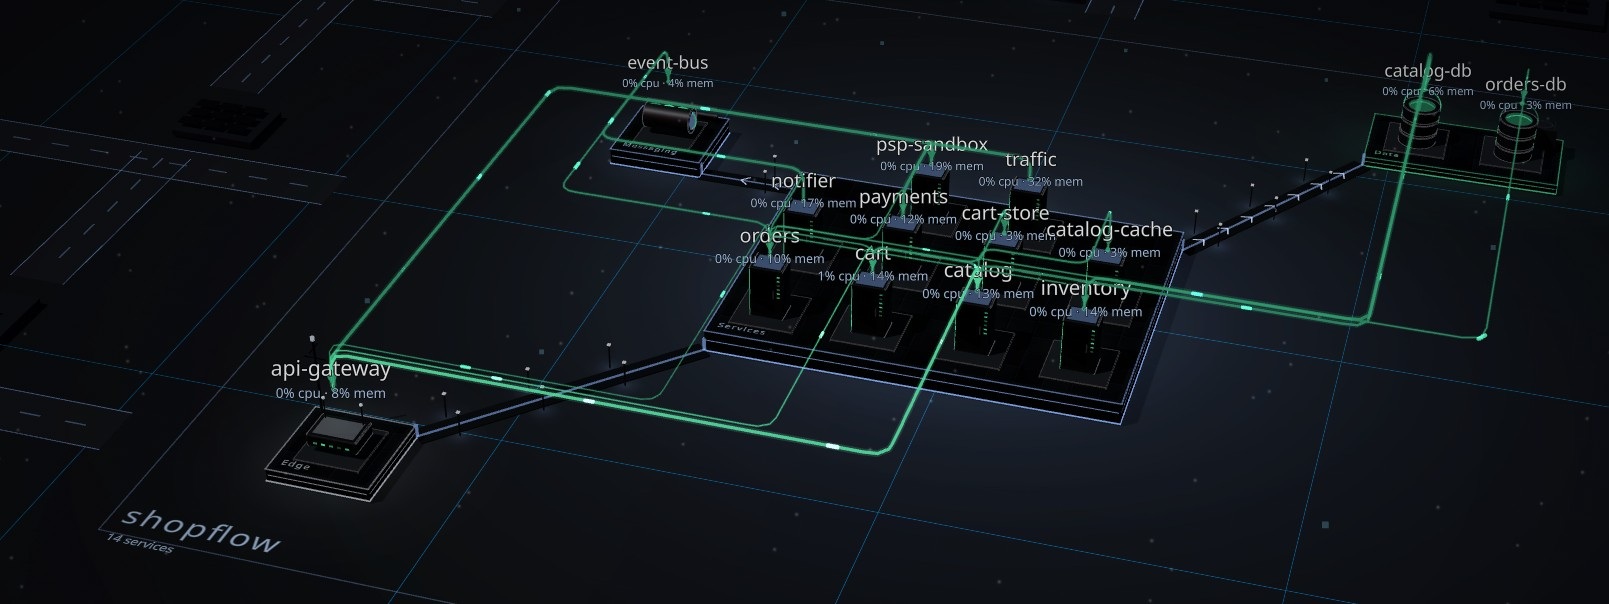
\includegraphics[width=0.84\textwidth]{ui3d_shopflow_islands_nocards.jpg}\\[3pt]
{\small (a) Islands}\\[6pt]
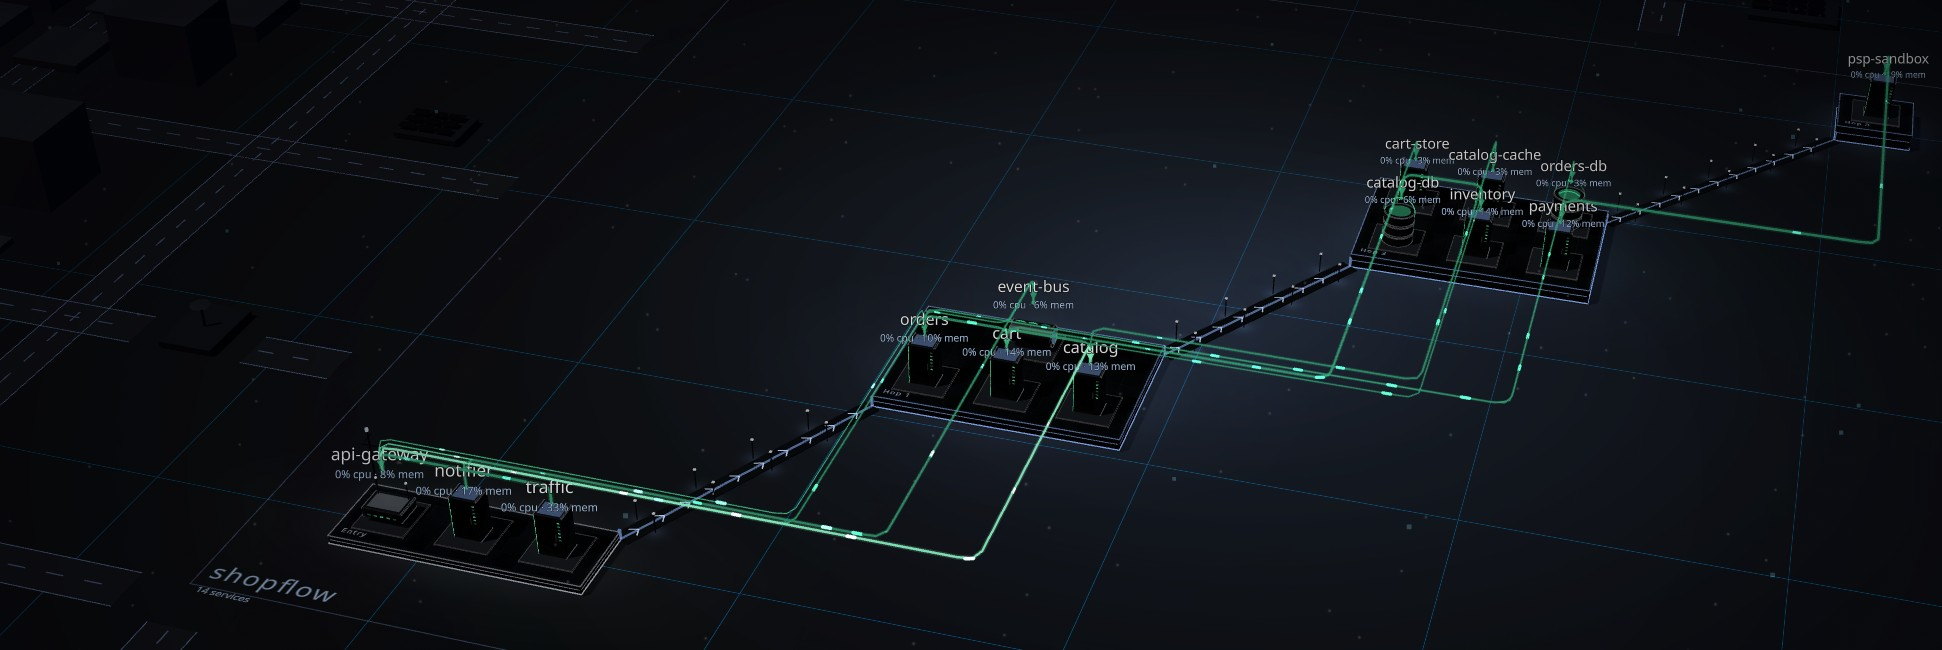
\includegraphics[width=0.84\textwidth]{ui3d_shopflow_flow_nocards.jpg}\\[3pt]
{\small (b) Flow}
\caption{ShopFlow in two of the four 3D arrangements.}
\end{figure}
\begin{figure}[H]
\centering
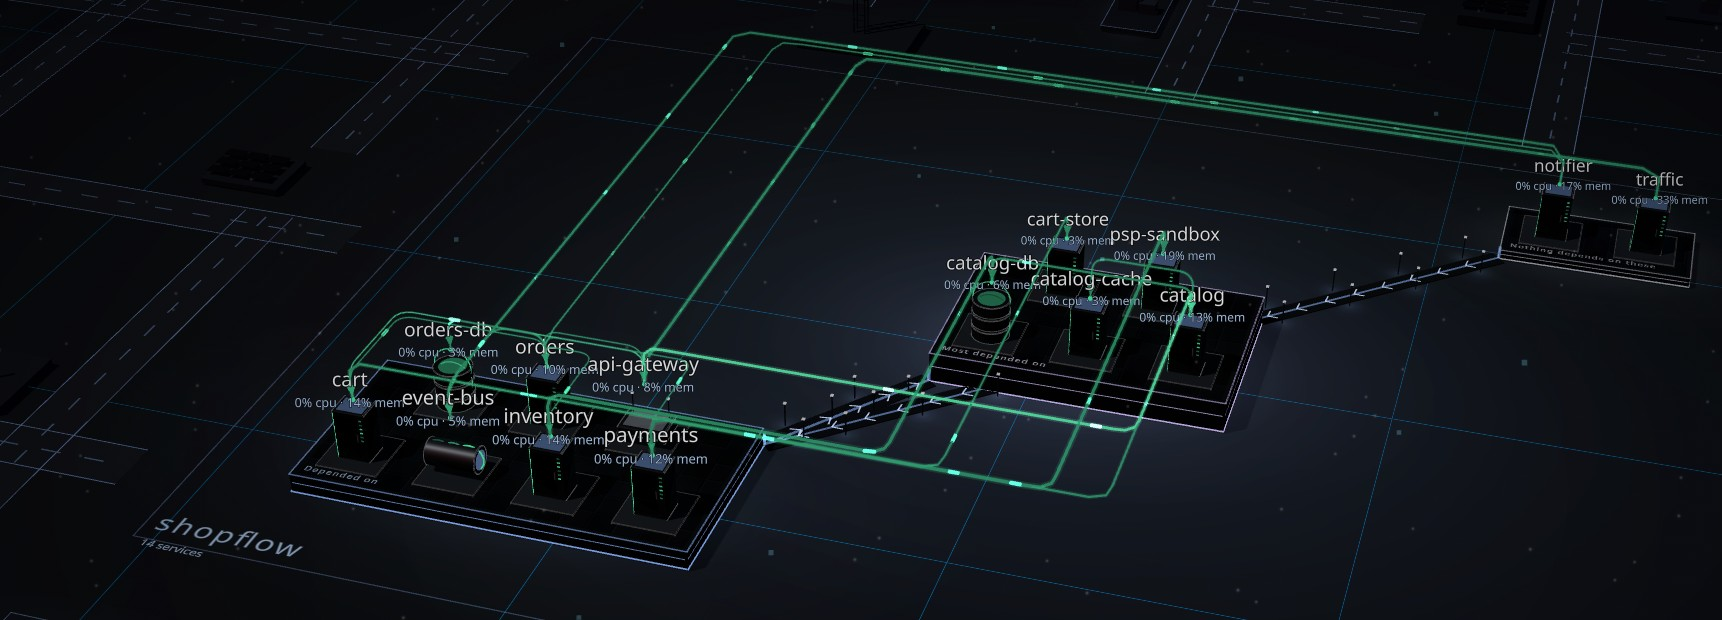
\includegraphics[width=0.84\textwidth]{ui3d_shopflow_topology_nocards.jpg}\\[3pt]
{\small (c) Topology}\\[6pt]
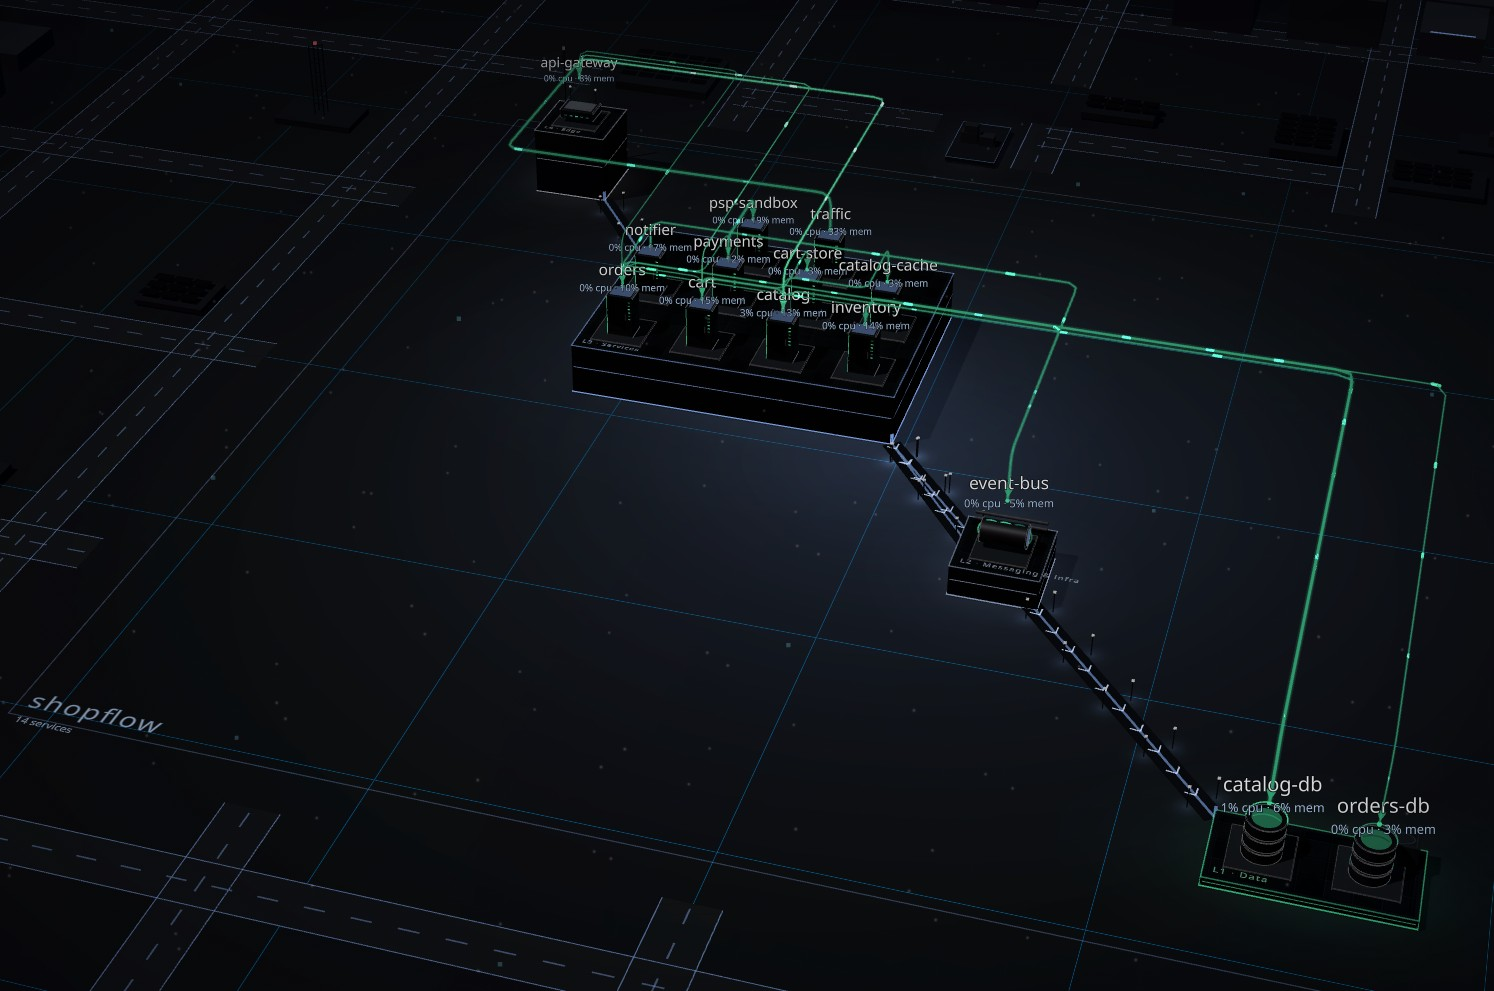
\includegraphics[width=0.62\textwidth]{ui3d_shopflow_tiers_nocards.jpg}\\[3pt]
{\small (d) Tiers}
\caption{ShopFlow in the other two arrangements.}
\end{figure}
\begin{figure}[H]
\centering
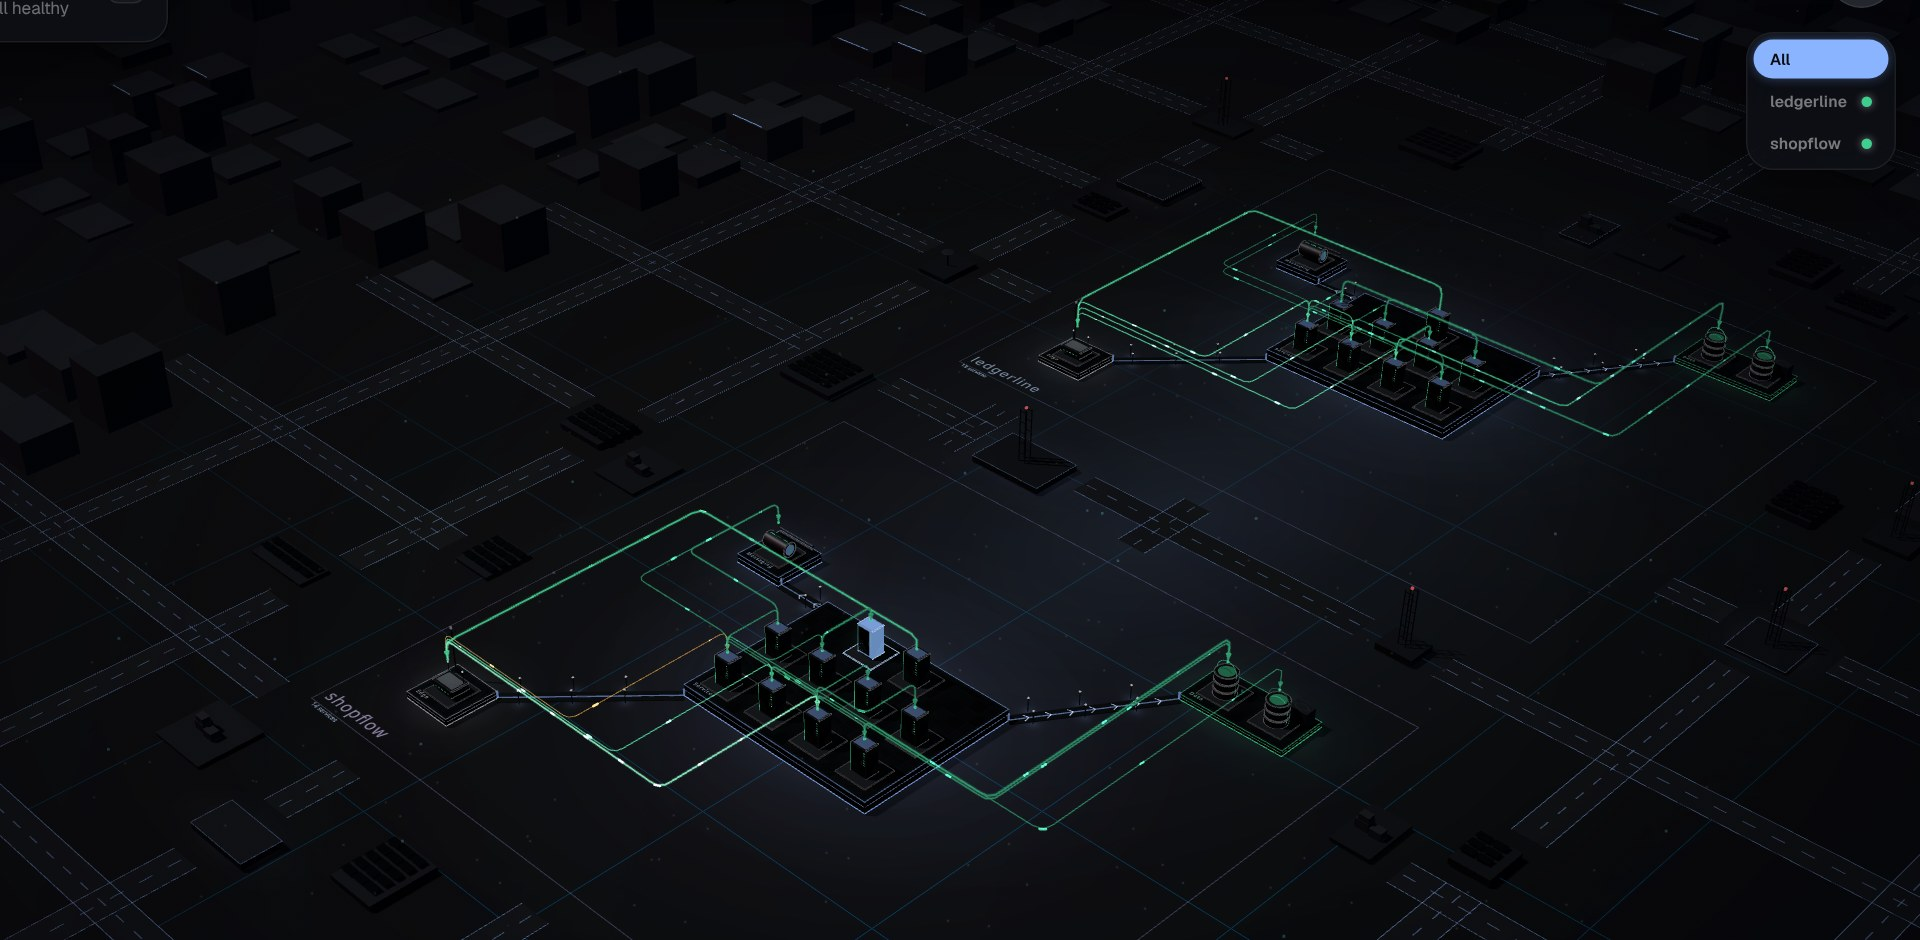
\includegraphics[width=0.9\textwidth]{ui3d_all_nocards.jpg}\\[3pt]
{\small (a) All projects}\\[6pt]
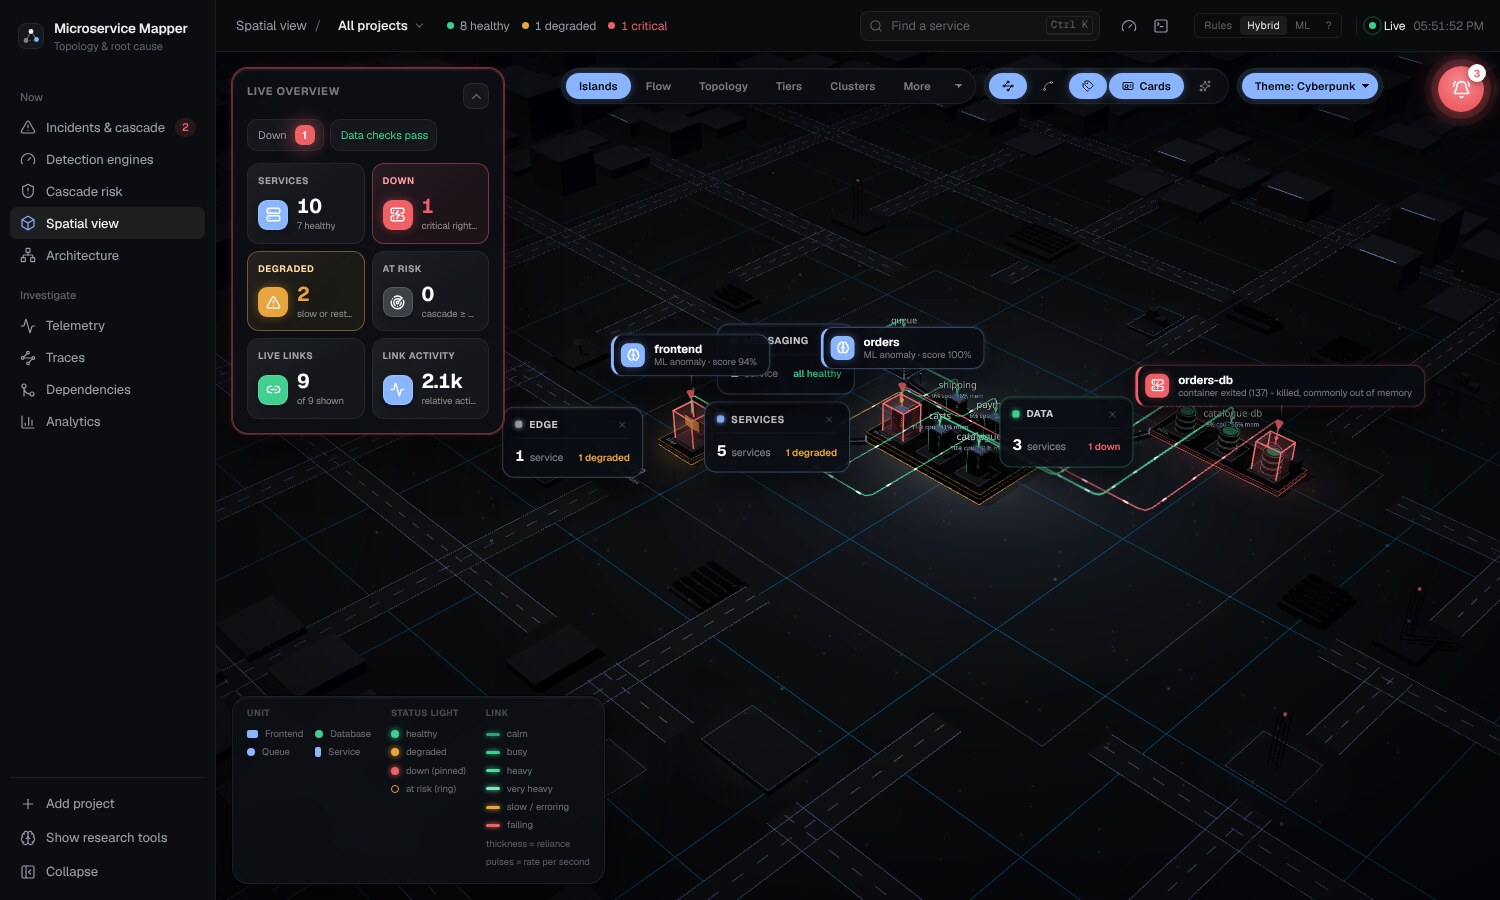
\includegraphics[width=0.9\textwidth]{ui3d_islands_fault.jpg}\\[3pt]
{\small (b) ShopFlow during a fault: \code{payments} paused}
\caption{The Islands view of all projects, and a fault in one of them.}
\end{figure}

\begin{saybox}
``Islands for what we have, Flow for how a request travels, Topology for what hurts most if it breaks, Tiers for whether the layers are respected. During a fault the failing unit is boxed in red with its name and score, and the bell in the corner counts what needs attention.''
\end{saybox}

\begin{techbox}
The scene is built with Three.js through react-three-fiber. Link thickness encodes the dependency weight and colour the heat of the link (calm, busy, heavy, very heavy, slow/erroring, failing); pulse rate is driven by the link's request rate. The legend on screen gives the status lights: green healthy, orange degraded, red down, and a ring for a service the cascade model marks at risk; a unit that the ML engine flags gets a callout with its name and anomaly score. Themes: Cyberpunk, Studio, Hologram. The camera frames the content automatically and flies to a zone or a service when selected.
\end{techbox}

\chapter{How we tested it: the evaluation design}
\label{ch:eval}

\section{The ground rules: what makes a test fair}
\begin{simplebox}
A fair test has four rules. (1) \textbf{The answer key is hidden.} The tool must not be able to peek at what was actually broken. (2) \textbf{The faults are physical.} We really kill, pause and starve containers, we do not just edit numbers. (3) \textbf{The test set is separate from the tuning set.} You do not grade a student on the questions you taught them with. (4) \textbf{Report the whole picture.} Include the weak results, with error bars.

We followed all four, within the limits we describe honestly later.
\end{simplebox}

\section{The two real systems we built}
\begin{simplebox}
We did not use someone else's demo app. We built two realistic systems, each in its own repository, each on its own cloud machine:

\begin{itemize}
\item \textbf{ShopFlow}: an online shop checkout with 13 services (a gateway, catalogue, cart, inventory, payments, orders, a notification consumer, a pretend third-party payment provider, plus databases, caches and a message bus).
\item \textbf{LedgerLine}: a bank-transfer system with 12 services (an edge, accounts, transfers, fraud screening, FX rates, a double-entry ledger, a statements worker, a pretend third-party FX provider, plus databases and a message bus).
\end{itemize}

Each comes with a monitoring stack (Prometheus, Grafana, Loki), an always-on traffic generator that mimics visitors with a daily wave, bursts and flash crowds, and a \emph{Fault Lab}: the fault injector.
\end{simplebox}

\begin{techbox}
Each bench runs on an EC2 \code{c7i-flex.large} host (2 vCPUs, 4\,GiB; about 0.6\,GiB of containers) in \code{ap-south-1}. The code of both is deliberately correct and defensive: every failure comes from configuration, data volume, sizing, topology or a third party, and every scripted scenario ships with a machine-readable ground truth (true root cause, what a monitor should and should not see, the fix). Monitoring is a \emph{separate Compose project}, so the application project stays exactly what a mapper should discover. A ``dashboard viewer'' container queries Grafana every few seconds, as a person watching would, so those links are live.
\end{techbox}

\begin{figure}[H]
\centering
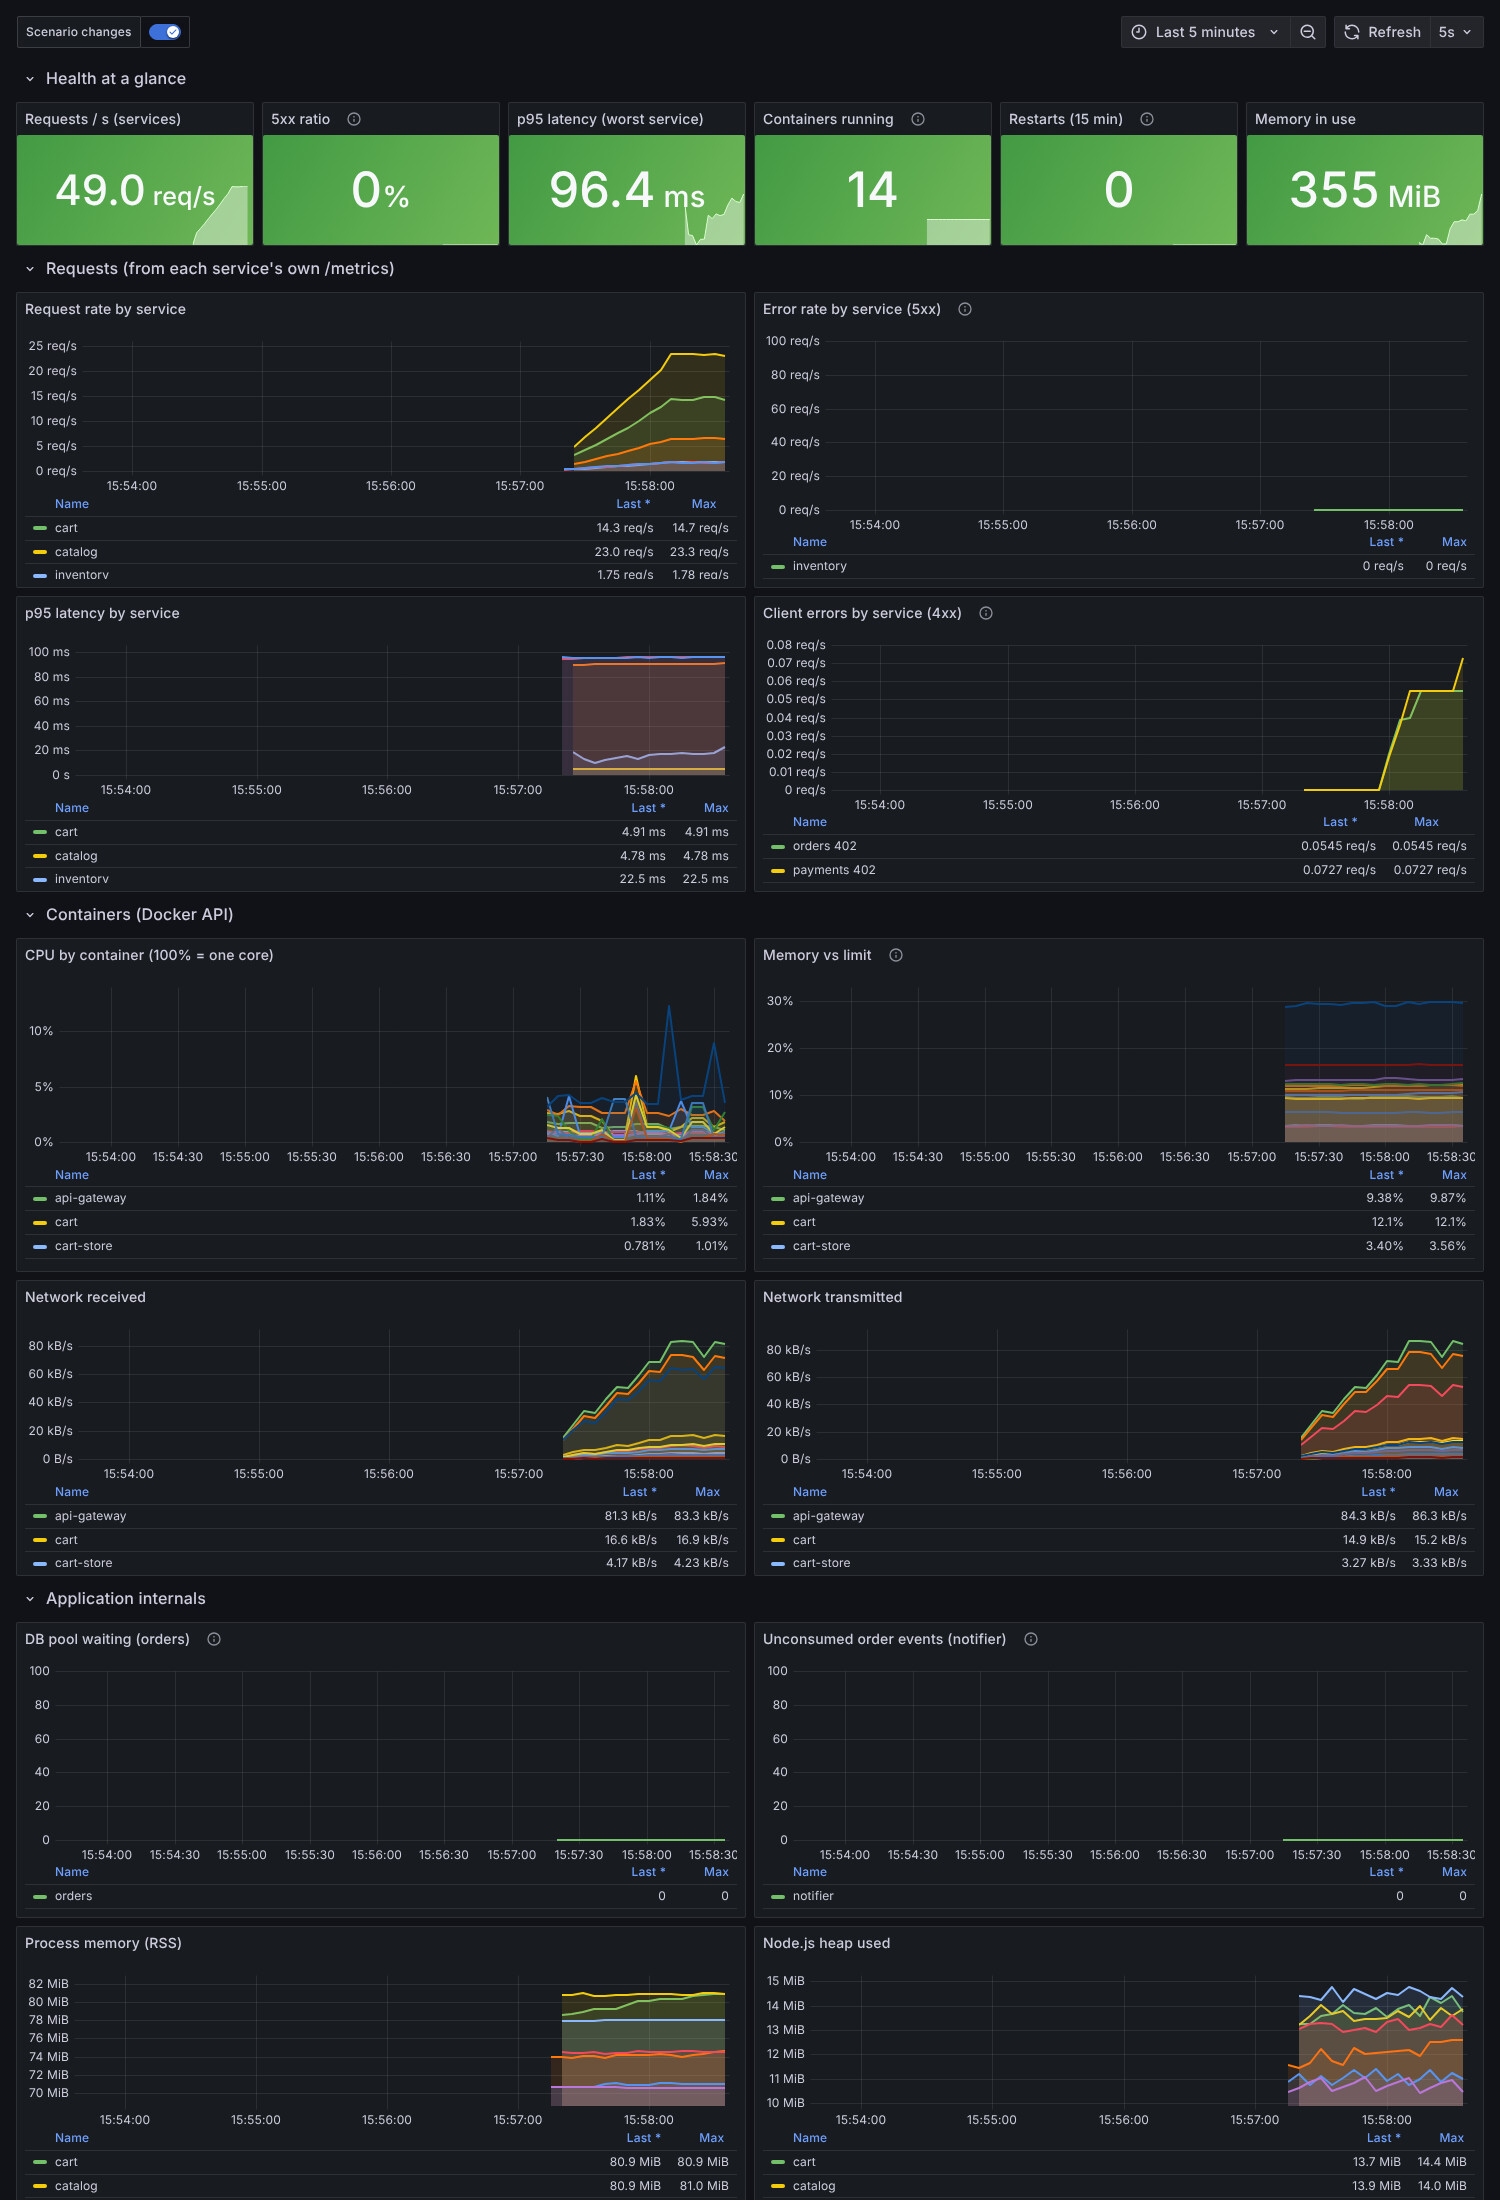
\includegraphics[width=0.5\textwidth]{grafana_shopflow.jpg}\hfill
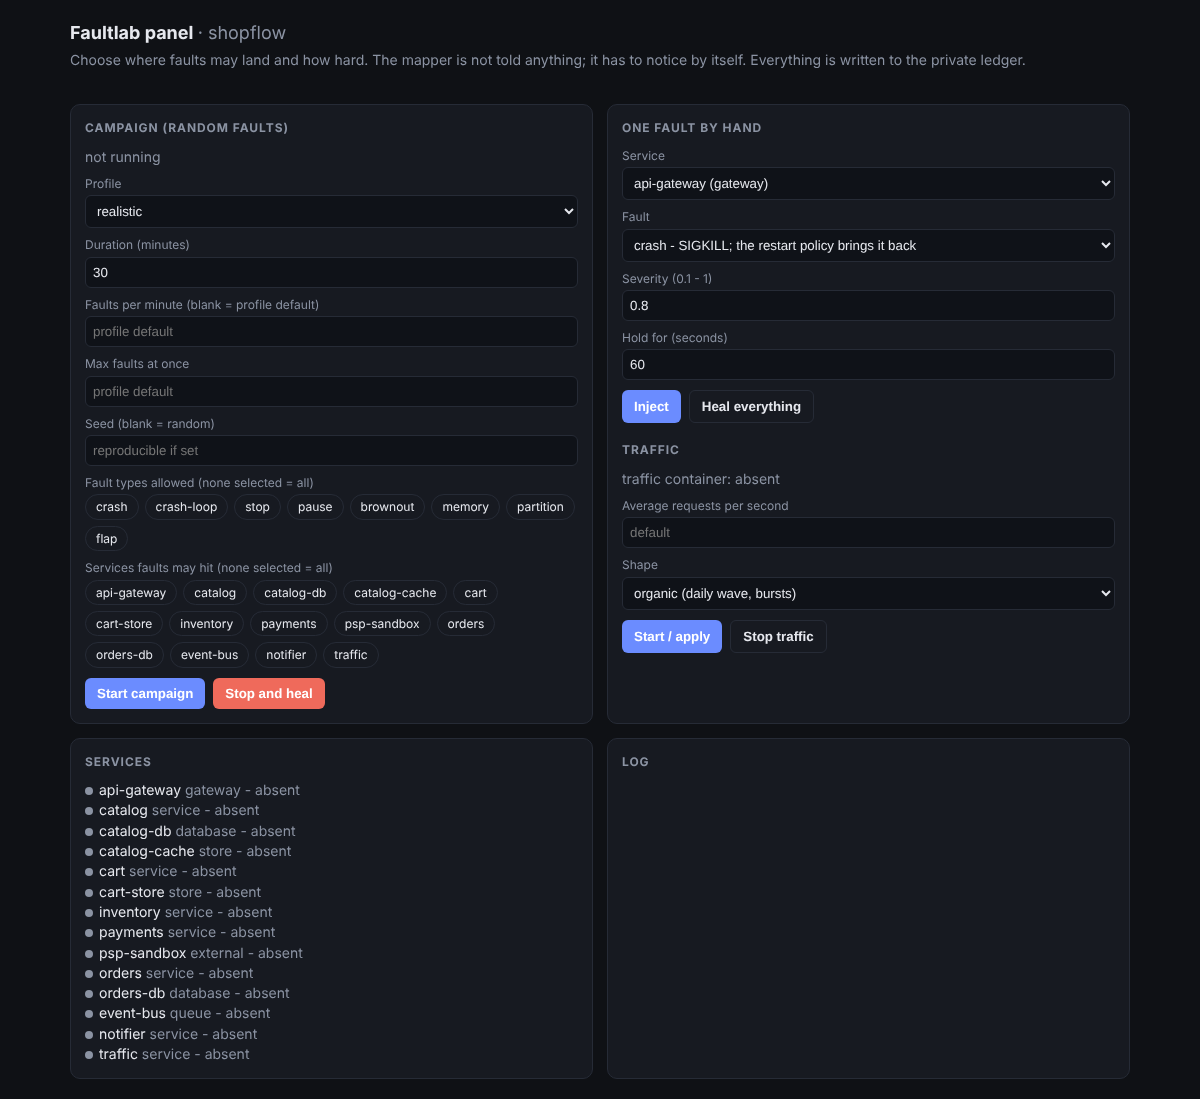
\includegraphics[width=0.46\textwidth]{faultlab_shopflow.png}
\caption{Left: the ShopFlow Grafana dashboard. Right: the Fault Lab control page.}
\end{figure}

\section{The Fault Lab: three properties}
\begin{simplebox}
\textbf{Blind.} The mapper is never told what is injected. The injector writes every fault into a private notebook (a ``ledger'') that nobody reads until scoring. \textbf{Physical.} Faults act on containers: kill, repeated kills, stop, pause, resource limits that slow a service, network detach, repeated pause-and-release. \textbf{Reproducible.} A campaign draws faults at random from a Poisson process with a profile, rate and seed; the same seed gives the same campaign.
\end{simplebox}

\begin{techbox}
Faults arrive by a non-homogeneous Poisson process whose rate follows the load, each with a class, a role-weighted target, a heavy-tailed duration and a severity; with some probability a follower is spawned in the target's one-hop neighbourhood, so incidents overlap. The ledger records, per fault, the true root cause and the services structurally able to be affected. The control page runs on the bench host, listens on localhost only and requires a header only the page itself sets, so another site open in the same browser cannot drive it. The two real systems contribute 62 faults over seven classes (crash, stop, brownout, memory, crash-loop, pause, flap).
\end{techbox}

\section{Four kinds of data}
\begin{center}
\small
\begin{tabularx}{\textwidth}{>{\raggedright\arraybackslash}p{2.7cm}>{\raggedright\arraybackslash}p{2.7cm}>{\raggedright\arraybackslash}X}
\toprule
\textbf{Data} & \textbf{Size} & \textbf{What it is for}\\
\midrule
Real recorded campaigns & 62 faults, 217 min each, both benches & The main result on real systems.\\
Live campaigns & 84 faults (21 per run; both benches; auto-restart on and off) & Check the mapper against a system it cannot see into, and test auto-restart.\\
Synthetic held-out & 178 faults, 16 topologies, seed 2, scored once & Enlarge the sample; test generalisation to topologies not tuned on.\\
Synthetic tuning & 170 faults, 16 campaigns, seed 1 & Choose settings; never used for reported numbers.\\
Workload recordings (no fault) & 62 min organic on/off; 72 min stepped $2,8,2,0,20,2$ visitors & Count false alarms when only the load changes; every alarm is false by construction.\\
\bottomrule
\end{tabularx}
\end{center}

\begin{warnbox}
The 62 real faults are not tuned on a held-out real system. Say ``the synthetic numbers come from a split scored once; the real numbers are optimistic by an amount we cannot measure''. Also: the workload recordings come from traffic generators, not real users.
\end{warnbox}

\section{The measures}
\begin{simplebox}
We needed measures that match how an operator experiences the tool, so we did not use a simple ``percentage of readings classified correctly''. We use event-level measures.

\begin{itemize}
\item \textbf{Detected}: an alarm names a truly involved service while the fault is active.
\item \textbf{Caught and named (C+N)}: detected, \emph{and} the true root cause was ranked first. This is the headline number.
\item \textbf{A@1, A@3}: among detected faults, how often the truth was first, or in the top three.
\item \textbf{False-alarm episodes per fault-free hour (FA/h)}: alarms outside every fault window, with one unbroken alarm counting as one episode.
\item \textbf{Alarm time}: the share of fault-free time the engine spent in alarm.
\item \textbf{Detection delay}: seconds from fault onset to the first alarm.
\end{itemize}

Why two false-alarm measures? One unbroken alarm counts as one episode, so an engine can look good on episodes while alarming almost all the time. Alarm time exposes that. An earlier version of our own detector had a low episode rate and 86\% alarm time on the real systems; after the refinements it was 5\%.
\end{simplebox}

\begin{techbox}
Point-wise scoring with a window adjustment (credit a whole event if any point is flagged) rewards an engine that flags one point of a long fault; that is not how an operator experiences an alarm. Warm-up (the first five minutes of each run) is excluded from false-alarm and ROC counts. Intervals are 95\% percentile bootstrap intervals over faults; comparisons between engines are \emph{paired} bootstrap differences over the same faults with two-sided $p$ values. Overlapping faults within a run are not independent, so intervals are, if anything, optimistic. With 62 real faults a difference below about 8--10 points cannot be resolved.
\end{techbox}

\section{What a bootstrap confidence interval means (so you can explain it)}
\begin{simplebox}
We have 62 faults and the tool caught and named 44 of them (71\%). Is the true rate 71\%? Not exactly: with a different 62 faults we would have got a slightly different number. To see how much the number wobbles, we pretend our 62 faults are the whole world, draw 62 faults \emph{with replacement} many times, compute the rate each time, and read off the middle 95\% of those rates. That range is the confidence interval. For 71\% on 62 faults it is about $[60, 81]$.
\end{simplebox}

\begin{examplebox}[A paired comparison in one paragraph]
To ask ``is Hybrid better than Rules?'' we do not compare two separate intervals. We look at the \emph{same} 62 faults under both engines. For each fault, record whether Hybrid got it and Rules did not (+1), the reverse ($-1$) or both/neither (0). Average these differences, and bootstrap the average. The result is $+8.1$ points, 95\% interval $[-1.6,+17.7]$. The interval includes zero, so we cannot rule out ``no difference'', and the $p$ value is 0.117 (not below 0.05).
\end{examplebox}

\section{Two measurement bugs, which we found and fixed}
\begin{simplebox}
\textbf{Bug 1: the notebook was half-read.} Each recorded run held two fault campaigns, and both numbered their faults from one. Our reader kept only the second, so for every engine 14 of 31 faults per system were hidden, and the outages of the hidden faults were counted as \emph{false alarms}. Every number in the report uses all 62 faults now, and a test guards the reader.

\textbf{Bug 2: the replay threw away the quiet parts.} The tool that replays recorded runs skipped a reading when it matched the previous one. An idle service reports the same zeros again and again, so the replay deleted exactly the idle stretches. That is why the old forest looked fine in our benchmarks when traffic stopped; the live system does not skip readings. We fixed the replay and recomputed every number that depended on it.
\end{simplebox}

\begin{saybox}
``Both bugs made the engines look \emph{better} than they were, and we found them ourselves. That is why we trust the numbers in the report: they are what is left after we tried to break our own evaluation.''
\end{saybox}

\chapter{The results, and what each one really says}
\label{ch:results}

\section{The main table}
\begin{center}
\scriptsize
\setlength{\tabcolsep}{3pt}
\begin{tabular}{lcccccc}
\toprule
Engine & Detected [95\% CI] & A@1 & A@3 & C+N [95\% CI] & FA/h & Alarm \%\\
\midrule
\multicolumn{7}{l}{\textit{Real benches (62 faults, 217 min)}}\\
Rules & 90 [82, 97] & 70 & 91 & 63 [52, 74] & 9.2 & 9\\
Severity ranking & 90 [82, 97] & 75 & 86 & 68 [56, 79] & 6.2 & 8\\
ML engine & 90 [82, 97] & 79 & 89 & 71 [60, 81] & 2.3 & 6\\
\textbf{Hybrid} & 90 [82, 97] & 79 & 89 & 71 [60, 81] & 6.2 & 8\\
Hybrid + change-point & 95 [89, 100] & 76 & 88 & 73 [61, 82] & 5.4 & 16\\
Hybrid + learned dir. & 90 [82, 97] & 75 & 89 & 68 [55, 77] & 6.2 & 8\\
\midrule
\multicolumn{7}{l}{\textit{Synthetic held-out (178 faults, 16 topologies)}}\\
Rules & 89 [84, 93] & 78 & 95 & 70 [62, 76] & 2.5 & 2\\
Severity ranking & 93 [89, 97] & 80 & 92 & 74 [67, 80] & 0.9 & 5\\
ML engine & 92 [87, 96] & 82 & 94 & 75 [69, 81] & 0.2 & 4\\
\textbf{Hybrid} & 93 [89, 97] & 81 & 93 & 75 [69, 81] & 0.9 & 5\\
Hybrid + change-point & 94 [90, 98] & 80 & 92 & 75 [69, 81] & 0.8 & 6\\
Hybrid + learned dir. & 93 [89, 97] & 81 & 93 & 75 [69, 81] & 0.9 & 5\\
\bottomrule
\end{tabular}
\end{center}

\begin{simplebox}
How to read it, row by row for the real benches. \textbf{Rules} found 90\% of faults, and named the right service first for 63\% of all faults, but they raised 9.2 false alarms per hour and were in alarm 9\% of the fault-free time. \textbf{ML} found the same 90\%, named the right service for 71\%, and raised only 2.3 false alarms per hour (6\% alarm time). \textbf{Hybrid} (the default) has the same 71\% but 6.2 false alarms per hour, because it also lets the rules raise the alarm. The two bold results to stress: ML and Hybrid have higher C+N than Rules, and ML has by far the fewest false alarms.
\end{simplebox}

\begin{techbox}
Paired differences (C+N): Hybrid vs Rules $+8.1$ points on the real systems (95\% CI $[-1.6,+17.7]$, $p=0.117$), $+5.6$ on the synthetic set ($[-0.6,+11.8]$, $p=0.093$); Hybrid vs severity ranking $+3.2$ and $+1.1$; Hybrid vs ML $0.0$ and $+0.6$. The first version of the report showed hybrid over rules as significant ($+9.7$ points, $p=0.032$). With the corrected engine it is not: the improvement is in robustness, not in the benchmark. With 62 real faults a difference below about ten points cannot be resolved.
\end{techbox}

\begin{figure}[H]
\centering
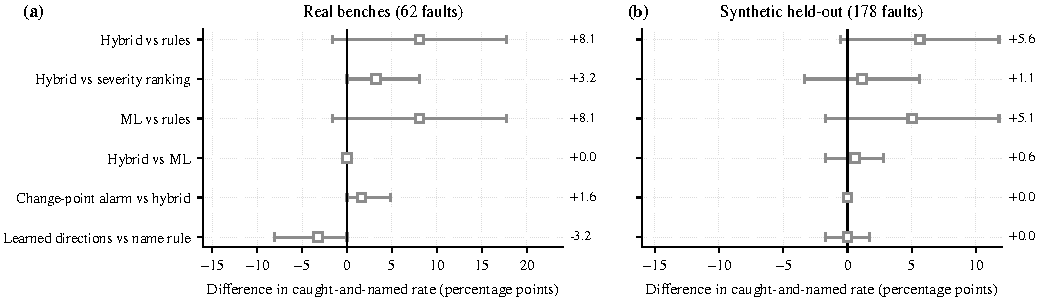
\includegraphics[width=0.98\textwidth]{fig_forest.pdf}
\caption{Paired differences in caught-and-named rate between engines (percentage points, 95\% paired-bootstrap interval); filled markers exclude zero.}
\end{figure}

\begin{figure}[H]
\centering
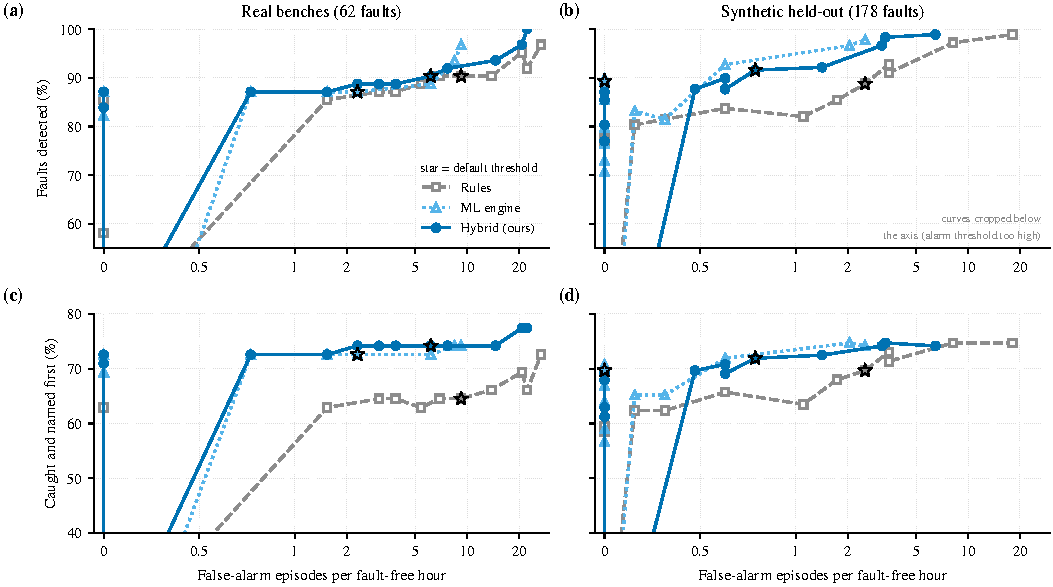
\includegraphics[width=0.98\textwidth]{fig_op.pdf}
\caption{Operating curves. Sweeping the alarm threshold of each engine traces detection rate (top) and caught-and-named rate (bottom) against false-alarm episodes per hour; stars mark the default threshold.}
\end{figure}

\begin{simplebox}
The operating curves show a different way to compare engines. Every engine has a dial (the alarm threshold). Turning the dial up trades faults caught for fewer false alarms. If you plot that trade for every engine, you see whether one engine is better at \emph{every} dial setting. Here the curves are close, and Hybrid and ML sit on or near the top edge in both sets, above the rules at almost every false-alarm budget. So their advantage is about the \emph{operating point}, not one lucky threshold.
\end{simplebox}

\begin{saybox}
``Rules, ML and Hybrid are close on how many faults they catch, 90\% on the real systems. The difference is that ML and Hybrid name the right service more often, 71\% against 63\%, and ML does it with a quarter of the false alarms. The 71 against 63 is not statistically significant with 62 faults, and we say so.''
\end{saybox}

\section{The ablation: which part matters}
\begin{figure}[H]
\centering
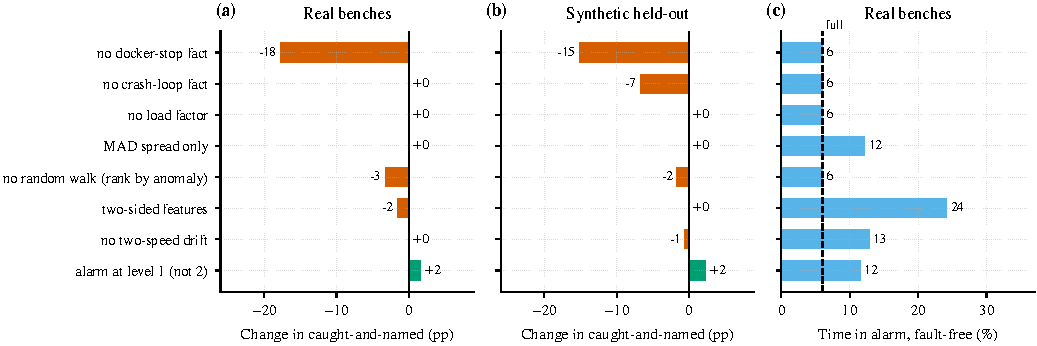
\includegraphics[width=0.98\textwidth]{fig_ablation.pdf}
\caption{Ablation. Each bar removes one mechanism from the full engine.}
\end{figure}

\begin{simplebox}
An ablation takes the full tool and removes one part at a time, to see what that part was worth. The parts are, in order of importance:
\begin{enumerate}
\item \textbf{The \code{docker stop} fact} costs \textbf{18 points} on the real systems and 15 on the synthetic set when removed, because every stopped service goes unnamed. This is the single most valuable component.
\item \textbf{The crash-loop fact}: 0 points on the real systems and 7 on the synthetic set.
\item \textbf{The random walk}: 3 and 2 points.
\item \textbf{The load factor}: nothing changes on injected faults (the load does not move in them); it matters on the workload recordings, where false alarms go from 0.0 to 1.2 and from 1.0 to 1.9 per hour without it.
\item \textbf{The tail-aware spread}: with the plain MAD spread, alarm time on the real systems doubles (6\% to 12\%), and on the workload recordings rises from 0\% to 10\% and 6\%.
\item \textbf{One-sided features}: removing them raises alarm time on the real systems from 6\% to 24\%.
\item \textbf{The two-speed drift}: without it, alarm time is 13\% instead of 6\% and false alarms 3.1 instead of 2.3 per hour.
\end{enumerate}
\end{simplebox}

\begin{saybox}
``The most important single component is container state as a fact: 18 points. The statistical mechanisms matter in a different way: they decide whether the model stays \emph{quiet}, not whether it \emph{catches} faults. Without the load factor nothing changes on the injected faults, but with it the false alarms on the workload recordings go from 1.2 and 1.9 per hour to 0.0 and 1.0.''
\end{saybox}

\section{Detection delay and top-$k$}
\begin{simplebox}
How fast does it react? On the real systems, the Hybrid's median delay from the start of a fault to the first alarm is 11.3 seconds, against 14.9 for the rules. On the synthetic set, whose faults are abrupt, it is 8.2 against 9.5 seconds. And among the detected faults, ML-based rankers put the true cause first more often than rules on the real systems (79\% against 70\%); by the third place both are near the 90\% ceiling. The remaining misses are mostly faults the engine \emph{does not see} (brownouts on near-idle services), not faults it ranks badly.
\end{simplebox}

\section{The service-level detection table}
\begin{center}
\small
\begin{tabular}{lcccc}
\toprule
 & \multicolumn{2}{c}{Real} & \multicolumn{2}{c}{Synthetic}\\
Detector & AUROC & AP & AUROC & AP\\
\midrule
Rule z-score & 0.695 & 0.337 & 0.873 & 0.666\\
Isolation Forest (old) & 0.629 & 0.288 & 0.862 & 0.528\\
k-NN & 0.668 & 0.193 & 0.860 & 0.517\\
Mahalanobis & 0.650 & 0.290 & 0.868 & 0.608\\
HBOS & 0.620 & 0.274 & 0.853 & 0.473\\
Ensemble of four & 0.650 & 0.287 & 0.865 & 0.593\\
Control chart (no load factor) & 0.669 & 0.302 & 0.842 & 0.657\\
Subspace residual & 0.696 & 0.298 & 0.847 & 0.629\\
Load-aware residual (new) & 0.665 & 0.313 & 0.842 & 0.665\\
\bottomrule
\end{tabular}
\end{center}
\begin{simplebox}
\textbf{AUROC} asks: if I pick one faulted service-moment and one healthy one at random, how often does the detector give the faulted one a higher score? 1.0 is perfect, 0.5 is coin-flip. \textbf{AP} (average precision) summarises how pure the top of the ranking is. The plain rule score is among the best on AUROC. That is fine: it ranks single readings well. It is not enough because it also fires on traffic swings and blames the loudest service.
\end{simplebox}

\section{The live campaigns and the auto-restart question}
\begin{center}
\small
\begin{tabular}{llrrrrr}
\toprule
Bench & Auto-restart & Detected & Top-1 (\%) & Top-3 (\%) & Delay (s) & FA/h\\
\midrule
ShopFlow & on & 100\% & 33 [17, 55] & 71 [50, 86] & 3.3 & 9.2\\
ShopFlow & off & 100\% & 24 [11, 45] & 71 [50, 86] & 2.6 & 0.0\\
LedgerLine & on & 95\% & 55 [34, 74] & 65 [43, 82] & 9.7 & 0.0\\
LedgerLine & off & 95\% & 40 [22, 61] & 70 [48, 85] & 3.9 & 3.1\\
\bottomrule
\end{tabular}
\end{center}
\begin{simplebox}
The same plan of 21 faults was replayed four times: both benches, with auto-restart on and off. Almost every fault was detected (all but one), and the true cause was within the top three suspects for 65 to 71\% of faults. The on/off rows differ by 9 to 15 points of Top-1, but with only 21 faults their intervals overlap completely, so none of the differences can be called an effect of auto-restart. \emph{Why was there no effect?} Because the benches set \code{restart: always} (Docker revives a crashed container within seconds, before the mapper looks), the mapper checks for dead containers only every 180 seconds (longer than the 20-second crash faults), and it skips containers that exited with code 0, which is what \code{docker stop} produces. The one restart in each ``on'' run was of the \emph{other} bench's message bus, which we had stopped by hand; that is an artefact of the setup and the report says so.
\end{simplebox}

\begin{techbox}
Direct test: \code{cart} and \code{payments} were each stopped for 5 minutes by the Fault Lab, sampled every 2\,s. Down time with auto-restart on/off: cart 299\,s / 298\,s, payments 301\,s / 301\,s. The mapper left the containers down in both modes. Brownouts are the weak class in all four runs (no Top-1 at all).
\end{techbox}

\section{The engines on one live fault (the simulator story)}
\begin{simplebox}
We also ran a simulator with a slow \code{payment} service (CPU saturated from second 30; \code{orders} follows twelve seconds later). It shows the personality of each engine on one fault.

\begin{center}
\small
\begin{tabularx}{\textwidth}{>{\raggedright\arraybackslash}p{1.6cm}>{\raggedright\arraybackslash}X>{\raggedright\arraybackslash}X>{\raggedright\arraybackslash}X}
\toprule
Engine & +5 s: payment only & +20 to +70 s: both saturated & after +75 s\\
\midrule
Rules & payment (3.0$\times$) & orders (3.7$\times$), payment second & the same\\
ML & payment (88\% of the walk) & payment (57\%), orders (43\%) & absorbed: no alarm\\
Hybrid & payment & payment (0.91), orders (0.87) & orders (alarm kept by the rules)\\
\bottomrule
\end{tabularx}
\end{center}

Rules point at the \emph{loudest} service (orders) once both are saturated. ML keeps blaming \code{payment} because its own CPU is the root, but then, because the fault is steady and mild, absorbs it after two minutes of simulated readings. Hybrid keeps the alarm up (from the rules) while naming the source mostly by ML.
\end{simplebox}

\begin{warnbox}
This is one simulated fault, an illustration and not evidence. It shows the mechanism the evaluation measures at scale. Do not use it as a result.
\end{warnbox}

\section{Operational findings from the benchmark hosts}
\begin{itemize}
\item \textbf{A host too small for its workload looks like a mapper fault.} The OpenTelemetry demo on a 2-vCPU, 4\,GiB instance had a load average near 25, 3.6 of 3.8\,GiB memory in use, and docker did not answer. The check tool measured it; the cure was a bigger host, not a mapper change.
\item \textbf{Idle front ends have no edges.} A front end that nothing calls has no outgoing sockets to see; an undeclared edge expires ten minutes after its last traffic.
\item \textbf{Hard-coded project names blocked traffic.} The traffic controller accepted only five named projects, so benchmark hosts with other names could not be driven. Unknown projects now get a generic workflow.
\end{itemize}

\section{Where we compare with published methods}
\begin{simplebox}
We did \emph{not} re-implement published root-cause systems (MicroRank, DiagFusion, Eadro and others) on our recordings. They need tracing in every service, or labelled failures and a GPU, which our setting does not have. So there is no head-to-head accuracy table against them, and we say that plainly. What we compared head-to-head are the \emph{baselines those methods build on}: the rule layer, ranking by anomaly alone, the walk, and a range of detectors.
\end{simplebox}

\chapter{What we cannot claim: limitations and honest answers}
\label{ch:limits}

An evaluator's best questions are about limits. If you have already said the limits yourself, those questions lose their sting. This part is the list, with a one-sentence reply for each.

\section{The limitation list, in plain words}

\begin{enumerate}
\item \textbf{We only see eight numbers per service.} A brownout on a nearly idle service moves none of them enough to alarm. No engine here catches it. \emph{Reply:} ``Outside-in observation is coarse by design; that is the trade for touching nothing. Active probing is listed as future work.''

\item \textbf{Two real systems.} We argue the method is architecture-independent from a cross-system check and from synthetic topologies, but we have not proved it. \emph{Reply:} ``Two systems we built, 217 minutes each, plus 16 random topologies. It is evidence, not proof.''

\item \textbf{Real cascades were rare.} Learned propagation could not be tested on real data because real faults are mostly absorbed single-service outages. \emph{Reply:} ``On synthetic cascades it is better calibrated. On real data there were too few cascades to say.''

\item \textbf{Edge evidence is not isolated offline.} The recordings do not keep it. \emph{Reply:} ``We use the evidence weighting live; we did not measure its isolated effect.''

\item \textbf{Cost was measured on synthetic readings.} Random graphs of 10--320 services on a shared virtual machine. \emph{Reply:} ``About 0.37 ms per service per window, linear; we have not observed a real system of that size.''

\item \textbf{Workload recordings are generated.} Traffic came from two generators, not real users, and a fault that begins during a very large change of load can be masked by the load-aware model. \emph{Reply:} ``That is why the Hybrid also lets the rules and container facts raise the alarm.''

\item \textbf{We tuned the settings.} Real-system settings were not tuned on a held-out real system, so those numbers are optimistic by an unmeasured margin. The load-model settings were swept on all recordings together. \emph{Reply:} ``We chose the flat region of the sweep, not its maximum, and the synthetic numbers come from a split scored once.''

\item \textbf{A mild fault longer than two minutes is absorbed by the ML.} The rules and container facts keep alarming. \emph{Reply:} ``A trade for not alarming forever on a service that really changed; we measured the alternative (4--20 minutes) and it doubled alarm time with no accuracy gain.''

\item \textbf{Early warning is weak.} Warned before the alarm for 13 of 178 synthetic faults and none of the 62 real ones. \emph{Reply:} ``It is the weakest component and we say so.''

\item \textbf{Auto-restart exists.} The mapper restarts crashed containers by default. \emph{Reply:} ``It had no measurable effect on our benches; switch it off when measuring detection.''

\item \textbf{Not tested on Kubernetes.}

\item \textbf{The ingest endpoint has a built-in token} for local use. \emph{Reply:} ``It must be changed when the server is reachable by others.''
\end{enumerate}

\section{The things that did not work (we reported them)}
\begin{simplebox}
An honest report lists failures. Ours does:

\begin{itemize}
\item The corrected ML engine is \emph{not} more accurate than the first at catching injected faults.
\item Hybrid over Rules was significant in the first version ($p=0.032$); with the corrected engine it is not ($p=0.117$).
\item The random walk is not significantly better than ranking by anomaly alone on our benchmarks.
\item Learned directions do not beat the name rule when names exist.
\item Onset-precedence re-ranking made no difference.
\item The subspace residual (the principled multivariate alternative) is as good at discrimination but raises more false alarms on the load steps and costs more.
\item Early warning does not fire on abrupt real faults.
\item A range guard on the new model added false alarms and was dropped.
\end{itemize}
\end{simplebox}

\section{Claims you should \emph{not} make}
\begin{warnbox}
\begin{itemize}
\item ``Our model is more accurate than the old one at detecting faults.'' (Same accuracy; it is more \emph{robust}.)
\item ``Hybrid is significantly better than rules.'' (Not significant.)
\item ``It predicts failures.'' (It forecasts \emph{who falls next} given a failure; early warning for gradual faults is weak.)
\item ``It works in production.'' (Two benches and a simulator; no production system.)
\item ``It is distributed tracing.'' (It is not.)
\item ``It is autonomous.'' (Its only action is a restart, which can be switched off.)
\item ``Learned propagation works on real cascades.'' (Untested on real cascades.)
\item ``We proved architecture independence.'' (Argued, not proven.)
\end{itemize}
\end{warnbox}

\section{Claims you \emph{can} make with confidence}
\begin{saybox}
\begin{itemize}
\item ``The first ML engine mistook a workload change for a fault: 23--52\% of the time in alarm on recordings with no faults. The corrected engine: 0\%.''
\item ``Container facts are the most valuable single component: 18 points on the real systems.''
\item ``The tool needs no labels, no GPU and no changes to the application; one decision costs about 0.37 ms per service.''
\item ``Learned propagation is better calibrated than fixed edge probabilities: ECE 0.033 against 0.051 on 69 cascades.''
\item ``Learned directions stay correct when names carry no information: 27 of 31 pairs, against none for the name rule.''
\item ``Two measurement bugs inflated the engines in our own benchmark; we found and fixed both.''
\end{itemize}
\end{saybox}

\chapter{The demo script}
\label{ch:demo}

A demo can go wrong in many small ways. This part gives two safe options: a \textbf{simulator demo} that needs only a laptop, and a \textbf{live-bench demo} that needs Docker and the benches. Practise the simulator one until it is boring; keep the live bench as the stretch goal.

\section{Before you start}
\begin{enumerate}
\item Node.js 20.19 or 22.12 and later. \code{npm run doctor} checks the machine.
\item In the repository, \code{npm start} installs what is missing and starts the server (port 3001) and the dashboard (port 5173). Open \code{http://localhost:5173}.
\item Keep a second terminal open for the simulator commands below.
\item Use a clean data folder for a demo so that old data does not confuse the story (the mapper keeps its data in \code{server/data}; never commit that folder).
\end{enumerate}

\begin{warnbox}
Never put \code{.pem} keys or the contents of \code{server/data} into git. The repository ignores them, but a stray \code{git add -A} in the wrong folder can still include data you do not want public.
\end{warnbox}

\section{Option A: the simulator demo (about ten minutes)}
\begin{simplebox}
The simulator pretends to be a small shop with ten services and scripted failures, so \emph{you know the true answer in advance}. That is useful in a demo: you can say ``watch, I will break the payment service'' and then show the tool finding it.
\end{simplebox}

\begin{techbox}
The simulator (\code{run/scripts/simulate-target.ts}) pushes telemetry to the mapper's real \code{/api/ingest} endpoint, the same path the SSH collector uses, so graph building, edge weights, detection, ranking, cascade prediction, the API and the UI all run for real. The target id is \code{sim-shop}. Scenarios: \code{baseline} (healthy), \code{db-crash} (\code{orders-db} exits with 137, then \code{orders} and the front end degrade), \code{slow-payment} (\code{payment} saturates, \code{orders} degrades after it), \code{crash-loop} (\code{carts-db} crash-loops, \code{carts} degrades). The ingest token defaults to \code{mapper-secret-token} unless \code{INGEST\_TOKEN} is set.
\end{techbox}

\subsection{The script, step by step}
\begin{enumerate}
\item \textbf{Start healthy.} In the second terminal run the baseline scenario for a few minutes:
\begin{verbatim}
node server/node_modules/tsx/dist/cli.mjs run/scripts/simulate-target.ts \
  --url http://localhost:3001 --token mapper-secret-token \
  --target sim-shop --scenario baseline --duration 200
\end{verbatim}
\emph{Say:} ``The mapper is learning what normal looks like. Everything is green.''
\item \textbf{Show the map.} Open \emph{Architecture} (2D) then \emph{Spatial view} (3D, \emph{Islands}). Point at the platforms and the cables.
\item \textbf{Break something.} Start the failure scenario:
\begin{verbatim}
node server/node_modules/tsx/dist/cli.mjs run/scripts/simulate-target.ts \
  --url http://localhost:3001 --token mapper-secret-token \
  --target sim-shop --scenario db-crash --duration 150
\end{verbatim}
\emph{Say:} ``I just killed the orders database. Watch the incident page.''
\item \textbf{Show the incident.} Open \emph{Incidents \& cascade}. Read it top to bottom: root cause, confidence, affected services, next in line, why, next steps.
\item \textbf{Show the three engines.} Open \emph{Detection engines}. Point at the three columns and the \emph{Peak against the alarm line} chart. Open it with the enlarge button.
\item \textbf{Tell the ML story.} ``This is the page that shows why we corrected the ML.'' Point at the workload chip. ``If the traffic changes, the chip says so, and no service is judged until it is explained.''
\item \textbf{Optional: the slow-payment scenario} shows Rules blaming the louder \code{orders}, while ML and Hybrid name \code{payment}.
\end{enumerate}

\begin{saybox}
At step 4, resist the urge to say everything. Say three things: ``this is the root cause and how sure we are, these are the services already hurt, these are the next ones''. Then stop and let them ask.
\end{saybox}

\section{Option B: the live-bench demo}
\begin{simplebox}
This runs a real application (the ShopFlow shop) in Docker on your machine, with the mapper watching it over SSH and the Fault Lab breaking containers while the mapper does not know. It is more impressive and more fragile. Do it only if the machine is ready and you have rehearsed.
\end{simplebox}

\begin{techbox}
The repository has a staged demonstration script: \code{npm run demo -- --bench ../bench-1 --subject shopflow}. Stages: (1) baseline (watch the running services so the mapper learns what normal is), (2) traffic (raise organic traffic $\times2$), (3) calm (random faults one at a time), (4) storm (faults more often, up to two at once), (5) score (compare the mapper's answers with the injector's private ledger into one HTML report). The mapper (\code{npm run local}) must already be running; the injector never talks to the mapper. Minutes are real time; use \code{--dry-run} to see the plan first.
\end{techbox}

\begin{warnbox}
\begin{itemize}
\item Allow thirty minutes of baseline in a real demo: the mapper needs about thirty readings per service before ML judges, and the learned rule model needs \code{MAPPER\_BASELINE\_MIN} (30) minutes.
\item Switch auto-restart off (\code{MAPPER\_AUTO\_RESTART=off}) so the mapper does not heal the faults you are showing.
\item On a laptop with little memory the benches are slow; check \code{docker ps} answers within a second or two before you start.
\end{itemize}
\end{warnbox}

\section{What to do if something goes wrong on stage}
\begin{center}
\small
\begin{tabularx}{\textwidth}{>{\raggedright\arraybackslash}p{4cm}>{\raggedright\arraybackslash}X}
\toprule
\textbf{What you see} & \textbf{What to do}\\
\midrule
Dashboard shows nothing & Check the server is on port 3001 (\code{curl localhost:3001/api/targets}). Run \code{npm run doctor}.\\
``Learning baseline 5 of 30 min'' stays up & That is normal for a new project. Use the simulator, or say ``the learned rules need thirty minutes; container facts work from the start''.\\
ML engine goes quiet during a slow fault & Expected: the two-minute drift rule absorbed a mild steady fault. Switch to Hybrid; say so.\\
A service shows a dash instead of a number & Expected: unmeasured is shown as missing, not as zero.\\
Host does not appear & Run \code{npm run check-host -- <ip> <key> <port>}; it says whether the host or the mapper is at fault.\\
3D view is slow & Turn off the glow button; use the Studio theme.\\
\bottomrule
\end{tabularx}
\end{center}

\chapter{The evaluator report, chapter by chapter}
\label{ch:reportmap}

The evaluator will hold the report (about 100 pages). This part tells you what is in each chapter, which pages of this guide explain it, and the one thing to say if they open that chapter.

\begin{center}
\small
\begin{tabularx}{\textwidth}{>{\raggedright\arraybackslash}p{3.1cm}>{\raggedright\arraybackslash}X>{\raggedright\arraybackslash}p{3.2cm}}
\toprule
\textbf{Report chapter} & \textbf{What it contains} & \textbf{Explained here}\\
\midrule
Abstract & Problem, what we built, the ML failure and fix, headline numbers. & Parts~\ref{ch:story}, \ref{ch:numbers}\\
1 Introduction & Background, problem statement, motivation, objectives, scope, contribution, organisation. & Parts~\ref{ch:story}, \ref{ch:problem}\\
2 Literature review & Anomaly detection, evaluation practice, root-cause localisation, cascade and change detection, benchmarks, observability tooling, comparison tables, the four gaps. & Part~\ref{ch:problem}\\
3 Proposed system and scope & Formal problem, seven-step solution, requirements, architecture, the two agents, three engines, components, design principles, scope. & Parts~\ref{ch:problem}, \ref{ch:system}\\
4 Methodology & Objective, measures, the models (graph, directions, load-aware model, hybrid, ranker, cascade, early warning), error sources, complexity, evaluation design, the two bugs. & Parts~\ref{ch:primer}--\ref{ch:more}, \ref{ch:eval}\\
5 Implementation & Environment, modules, algorithms, API, configuration, prototype screenshots, security, testing, the two benches and their Fault Lab, diagnostic tools, harness. & Parts~\ref{ch:observe}, \ref{ch:ui}, \ref{ch:eval}, \ref{ch:codemap}\\
6 Results & The ML correction, which model of normal, rules vs old vs new, detection and root cause, ablation, amplification, cascade, directions, early warning, cost, live campaigns, analysis, validity, comparison. & Parts~\ref{ch:mlstory}, \ref{ch:rank}--\ref{ch:more}, \ref{ch:results}, \ref{ch:limits}\\
7 Conclusion & Summary, conclusions, contributions, utility, limitations, future work. & Parts~\ref{ch:limits}, \ref{ch:qa}\\
Appendices & Engine constants, fault classes, user guide. & Parts~\ref{ch:demo}, \ref{ch:codemap}\\
\bottomrule
\end{tabularx}
\end{center}

\section{If they open a specific figure or table}
\begin{center}
\small
\begin{tabularx}{\textwidth}{>{\raggedright\arraybackslash}p{3.4cm}>{\raggedright\arraybackslash}X}
\toprule
\textbf{They open\ldots} & \textbf{Say\ldots}\\
\midrule
Architecture figure & ``One SSH connection, fixed read-only commands, nothing installed. Three engines run on the same readings; the switch only chooses which one opens incidents.''\\
Hybrid alarm figure & ``Alarm if a container fact holds, or the ML level is twice its line, or the rules are 25\% past theirs. The model and rule conditions must hold for two cycles.''\\
Cascade example figure & ``Edge probabilities are learned from the system's own incidents. Risk at the gateway combines two routes with noisy-OR.''\\
Workload figure (6.1) & ``Panel (a) is the traffic stepping up and down. Panel (b): the old forest alarms with the traffic, the new model does not. Panel (c) is the load factor the new model read.''\\
Models table and figure (6.2) & ``Look at the last two columns: forest family 23--96\% of calm time in alarm, adopted model 0\%. The injected-fault columns are all close.''\\
Rules vs old vs new table & ``Same recordings, same replay, three engines. New ML is slightly ahead on injected faults with far fewer false alarms, and clearly ahead when only the workload moves.''\\
Main table (6.3) & ``Detection is 90\% for all engines on the real systems. ML and Hybrid name the right service more often. The difference is not significant with 62 faults.''\\
Operating curves & ``Sweep the alarm threshold: the engines trace nearly overlapping curves, and Hybrid and ML sit on the upper edge.''\\
Ablation & ``The stop fact is the single most valuable component, 18 points. The statistical mechanisms decide whether it stays quiet.''\\
Amplification study & ``As victims get louder, severity ranking falls and the walk holds, but intervals include zero at every level.''\\
Cascade calibration & ``Better calibrated than fixed probabilities on synthetic cascades; real cascades were too rare to test.''\\
Early warning & ``The weakest part. Works for some gradual synthetic faults; did not fire on abrupt real ones.''\\
Cost figure & ``Linear in the number of services, 0.37 ms per service; far below the 5-second period.''\\
Live campaign table & ``Same plan, four runs, auto-restart on and off. Intervals overlap completely: no measurable effect.''\\
3D figures & ``Islands, Flow, Topology and Tiers: four questions a developer asks. Shown without the cards because cards can cover units.''\\
Engines page screenshot & ``Rules blame the louder victim; ML and Hybrid name the source and say why.''\\
\bottomrule
\end{tabularx}
\end{center}

\chapter{Presenting as a team of four}
\label{ch:roles}

An evaluator will ask any of you anything. But a presentation goes best when each person owns a part and the hand-offs are clean. This is a suggested split by topic, not by who wrote which code. Change it to fit who knows what, but make sure \emph{every} part of this guide is owned by at least two people, so nobody is stranded if one of you is asked a question outside their part.

\section{A suggested split}
\begin{center}
\small
\begin{tabularx}{\textwidth}{>{\raggedright\arraybackslash}p{2.2cm}>{\raggedright\arraybackslash}p{4.4cm}>{\raggedright\arraybackslash}X}
\toprule
\textbf{Speaker} & \textbf{Owns} & \textbf{Guide parts}\\
\midrule
Speaker 1 & The problem and the big picture: story, why existing tools do not fit, what the system is, the architecture and the three engines. Also the opening and closing. & \ref{ch:howto}\ (how to use), \ref{ch:story}, \ref{ch:problem}, \ref{ch:system}\\
Speaker 2 & Observation and the graph: SSH, sockets, direction, container facts, edge confidence, learned directions, the dashboard and the 3D tour. & \ref{ch:observe}, \ref{ch:graph}, \ref{ch:ui}\\
Speaker 3 & The detection and ML story: rules, the old forest, why it failed, the load-aware model, the comparison, and the three-way table. & \ref{ch:primer}, \ref{ch:detect}, \ref{ch:mlstory}\\
Speaker 4 & Ranking, cascade, evaluation and results: root cause, noisy-OR, the Fault Lab, the measures, the main table, ablation, limits. & \ref{ch:rank}, \ref{ch:cascade}, \ref{ch:more}, \ref{ch:eval}, \ref{ch:results}, \ref{ch:limits}\\
\bottomrule
\end{tabularx}
\end{center}

\section{A ten-minute talk with hand-offs}
\begin{center}
\small
\begin{tabularx}{\textwidth}{>{\raggedright\arraybackslash}p{1.5cm}>{\raggedright\arraybackslash}p{1.8cm}>{\raggedright\arraybackslash}X}
\toprule
\textbf{Minutes} & \textbf{Speaker} & \textbf{Content}\\
\midrule
0:00--1:30 & 1 & The restaurant story, the problem, why current tools do not fit. Hand-off line: ``To do this from outside, we first need to see the system. Over to \ldots''\\
1:30--3:00 & 2 & SSH and sockets, who calls whom, container facts. Show the 3D Islands view. Hand-off: ``Seeing is not enough, we must decide what is wrong.''\\
3:00--5:30 & 3 & Normal is personal; the first ML failed (23--52\%); the load-aware fix; the chart on the Detection engines page. Hand-off: ``Once we know something is wrong, who started it?''\\
5:30--7:00 & 4 & The decomposition, the random walk, noisy-OR prediction, a live break in the simulator.\\
7:00--9:00 & 4 then 1 & Evaluation: blind Fault Lab, the measures, the headline results with the honest caveat. Then back to 1.\\
9:00--10:00 & 1 & Limits and future work, and the one-sentence takeaway: ``Test your detector when nothing is wrong.''\\
\bottomrule
\end{tabularx}
\end{center}

\section{Rules for the question time}
\begin{enumerate}
\item The person who owns the topic answers first. If they stumble, a teammate may add one sentence, not take over.
\item Answer the question that was asked. Use the short version from Part~\ref{ch:qa} and stop.
\item If you do not know, say ``we did not measure that; the closest thing we measured is \ldots''. Do not invent a number.
\item Never argue with an evaluator about whether something is a limitation. Say ``agreed, it is listed under limitations''.
\item If an evaluator finds a mistake in the report, thank them and say how you would check it. Do not defend an error.
\item Keep these three honesty sentences ready: ``the 71 against 63 is not significant'', ``our first ML called every workload change a fault'', ``we found two bugs in our own measurement''.
\end{enumerate}

\section{The night-before checklist}
\begin{itemize}
\item Run the simulator demo end to end once on the machine you will present on.
\item Open the PDF report and this guide on a second screen.
\item Know your own five numbers (Part~\ref{ch:numbers}).
\item Check that auto-restart is off if you plan to show a live fault on a bench.
\item Charge the laptop and have the PDF on a USB stick.
\item Sleep.
\end{itemize}

\chapter{Questions an evaluator may ask, with answers}
\label{ch:qa}

Each answer has a \textbf{short version} (what to say first) and, when useful, a \textbf{longer version} (if they push). Say the short version, stop, and wait. Do not volunteer the long one unless asked.

\section{The project in general}

\q{What problem does your project solve?}\\
\textbf{Short:} When one service in a microservice system fails, the failure spreads and the engineer gets dozens of alarms without knowing which service started it. Our tool finds the likely root cause and predicts which services fall next, without changing the application.\\
\textbf{Longer:} It watches the Docker containers from outside over SSH, builds the call graph from socket tables, judges every service against its own normal, ranks causes with a random walk and spreads risk with a learned noisy-OR cascade model.

\q{What is new here? Others have done root-cause analysis.}\\
\textbf{Short:} Three things together. It works with no instrumentation and no labels, on one CPU core. The cascade model learns edge probabilities online. And our evaluation is blind, event-level and reports negative results.\\
\textbf{Longer:} Many published methods need traces, labelled failures or GPUs. The random-walk family needs only a graph and an anomaly score, and we build on that. Our contributions: recovering the graph and call direction from the host alone, a load-aware model of normal that does not confuse a workload change with a fault, facts-first ranking, learned propagation, and an honest evaluation that includes two measurement bugs we found.

\q{Why did you not use deep learning?}\\
\textbf{Short:} Deep models need labelled failures and GPUs, and the engineer cannot audit their output. Our users have neither labels nor GPUs, and need to see why.\\
\textbf{Longer:} Also, the simple models beat or matched the complex ones in our own comparison of nine models of normal. The key problem (workload changes) was not about model capacity; it was about what the model assumes.

\q{Is this AI?}\\
\textbf{Short:} It is unsupervised machine learning and probabilistic modelling, not a neural network and not a language model.\\
\textbf{Longer:} The learned parts: the model of normal per service, the edge propagation probabilities (Beta--Binomial), the learned call directions, the fault-type classifier (a random forest).

\q{What does ``agent-assisted'' mean?}\\
\textbf{Short:} A collector agent that observes and a diagnosis assistant that turns the observations into a cause, a forecast, a fault type and a runbook. Neither is a language model.

\q{Does it work on real systems?}\\
\textbf{Short:} On two real, containerised systems we built, running in Docker on cloud hosts, with 62 blind-injected faults over 217 minutes each, plus 84 live faults.\\
\textbf{Longer:} Not in production. We argue generality from a cross-system check and 16 synthetic topologies. We say plainly that it is evidence, not proof.

\section{Observation and the graph}

\q{How do you get the dependencies without instrumenting the application?}\\
\textbf{Short:} From each container's socket table, read over SSH through the host's \code{/proc}. A connection shows who is talking to whom.

\q{How do you know which service is the caller?}\\
\textbf{Short:} The end that holds the listening port is being called. The end with a random temporary port is the caller.\\
\textbf{Longer:} If the listening port is unknown we use the ephemeral-port range as a fallback with lower confidence (0.85). If neither settles it, the edge is marked unresolved (confidence 0.50). We never guess silently.

\q{Why does direction matter so much?}\\
\textbf{Short:} Failure travels against the arrow. If the arrows are wrong, every downstream question (root cause, cascade, blast radius) gives the opposite answer.

\q{What if the service names are meaningless?}\\
\textbf{Short:} Learned directions use how services behave during trouble. On 31 real pairs they are right for 27; the name rule is undecided for all of them when names are hidden.

\q{What are ``container facts''?}\\
\textbf{Short:} Container state treated as certainty, not as a degree of anomaly: stopped, paused, restarting, network-detached, crash-looping. When one exists, that service ranks first.\\
\textbf{Longer:} We added two facts that raw state misses: \code{docker stop} exits with code zero (looks like a finished job), and a crash loop looks healthy between kills. Removing the stop-fact costs 18 points on the real systems.

\q{Is anything installed on the monitored hosts?}\\
\textbf{Short:} No. One SSH connection and a fixed list of read-only Docker and \code{/proc} commands.

\q{Is it safe to give it SSH access?}\\
\textbf{Short:} The commands come from a fixed catalogue, every argument is sanitised, output and time are bounded, and keys stay on the operator's machine, never in the repository.\\
\textbf{Longer:} A test checks that an identifier with shell metacharacters is refused before a command is built. The one write the mapper makes is restarting a crashed container (non-zero exit), a few times at most, and it can be switched off.

\q{What are the eight metrics?}\\
\textbf{Short:} CPU, memory, CPU throttling, network in and out, request rate, error share and p95 latency, every five seconds.

\q{What happens when a metric is missing?}\\
\textbf{Short:} It stays missing and is never replaced by zero, because ``idle'' and ``not measured'' lead to opposite decisions.

\section{Detection and the ML correction}

\q{What was wrong with your first ML engine?}\\
\textbf{Short:} It flagged every service as anomalous when the traffic stopped, because it could not tell ``everyone got quieter'' from ``one service is sick''.\\
\textbf{Longer:} The Isolation Forests learn the shape of each service's recent readings. A workload change moves all services outside that shape together. On fault-free recordings it was in alarm 23\% to 52\% of the time.

\q{How did you find it?}\\
\textbf{Short:} An operator stopped the traffic generator and switched to ML, and every service showed 100\%. We then recorded fault-free runs with only the load changing and measured it.\\
\textbf{Longer:} Our own benchmarks had hidden it: the replay tool skipped repeated readings, which deleted the idle stretches.

\q{How does the new model avoid that?}\\
\textbf{Short:} It first estimates how much the whole project's workload moved (a median over busy services), expects each service to follow that, and judges only the leftover. A fault in one service cannot move a median.

\q{Why a median and not an average?}\\
\textbf{Short:} One broken service can drag an average but barely moves a median. The median follows the shared change and ignores the fault.

\q{What if a fault happens during a traffic change?}\\
\textbf{Short:} It is still seen, because each signal is tested against two hypotheses (ignores load / follows load) and counts as unusual only if neither explains it. A CPU spike on one service during a surge is still a spike compared with what the surge predicts.\\
\textbf{Longer:} But a fault that starts during a \emph{very large} load change can be masked. The Hybrid also lets the rules and container facts raise the alarm, which covers some of that.

\q{Is the new model more accurate than the old one?}\\
\textbf{Short:} At catching injected faults, about the same (71\% against 69\% caught and named on the real faults, inside the noise). The improvement is robustness: 0\% against 23--52\% time in alarm when only the load moves.

\q{Why did you choose the load factor over the control chart or the subspace model?}\\
\textbf{Short:} The control chart with the tail spread is almost as good (0\% and 0\% time in alarm) but still raised 1.2 and 1.9 false episodes per hour; with the load factor 0.0 and 1.0. The subspace model discriminates as well but raised 7.7--10.7 false episodes per hour on the steady load steps, adapts more slowly and costs more as services grow.

\q{What is the tail-aware spread?}\\
\textbf{Short:} The spread is at least the distance to the 90th percentile in the direction that matters, so a bursty signal's ordinary bursts count as normal width. Without it, alarm time on the workload recordings rises from 0\% to 10\% and 6\%.

\q{Why do you only accept readings below the alarm line into the training window?}\\
\textbf{Short:} So a long fault never becomes the baseline.

\q{What is the downside of that gate?}\\
\textbf{Short:} A mild fault that lasts more than two minutes is eventually absorbed. The rules and container facts keep alarming. We measured longer drift times and they doubled alarm time with no accuracy gain.

\q{Did you tune on the test data?}\\
\textbf{Short:} For the load model, partly: the alarm line, window and slow reference were swept over all recordings together; we chose the flat region, not the maximum. The synthetic numbers come from a split scored once. The real-system numbers have no held-out system, so they are optimistic by an unmeasured margin.

\q{Why is Hybrid the default if ML has fewer false alarms?}\\
\textbf{Short:} The Hybrid lets the rules and container facts also raise the alarm, so it covers what ML absorbs or cannot see, at the cost of more false alarms (6.2 per hour against 2.3 on the real systems).

\q{What does a false alarm mean in your evaluation?}\\
\textbf{Short:} An alarm episode outside every fault window, with one unbroken alarm counting as one episode. We also report alarm time, because an engine could meet an episode budget while alarming almost all the time.

\section{Ranking, cascade and prediction}

\q{How do you decide the root cause?}\\
\textbf{Short:} Two steps. First, split each service's trouble into what it caused itself (CPU, memory) and what it inherited (symptoms), subtracting what its sick callees explain. Second, a random walk over the call graph, which collects the most time at the true source. Facts rank first.

\q{Why is the loudest service often the wrong answer?}\\
\textbf{Short:} Victims accumulate symptoms from everything below them (retries amplify the load), so they can be louder than the origin.

\q{Is the random walk better than ranking by severity?}\\
\textbf{Short:} Not significantly on our benchmarks. Under an amplification study the walk holds at 75--76\% while severity falls from 76\% to 71\%, a gain growing to $+3.8$ points ($[-0.9,+9.4]$), but our sample is too small to confirm it.

\q{How does the cascade model work?}\\
\textbf{Short:} Each call edge has a probability that trouble crosses it. We learn it online: every time a service goes bad, each healthy caller is a trial, and it succeeds if it goes bad within a minute. A Beta--Binomial update gives the probability. Risk then spreads up the graph by noisy-OR.

\q{What is noisy-OR?}\\
\textbf{Short:} The chance a service is hit is one minus the product of the chances each route fails to deliver trouble. It combines independent routes.

\q{Is the learned cascade model better than a fixed probability?}\\
\textbf{Short:} Better calibrated: ECE 0.033 against 0.051 on 69 synthetic cascades; ranking only slightly better (AUROC 0.841 against 0.827). On real systems there were too few cascades to test.

\q{Do you predict failures before they happen?}\\
\textbf{Short:} We predict who falls next \emph{given} a failure. Early warning for gradual faults exists but is weak: it warned before the alarm for 13 of 178 synthetic faults and none of the 62 real ones, which were abrupt.

\q{What does the change-point alarm do?}\\
\textbf{Short:} It cuts the median detection delay on the real systems from 11.3 to 4.8 seconds, but doubles the time in alarm (8\% to 16\%), so it is a trade-off and not the default.

\q{How do you name the fault type?}\\
\textbf{Short:} A random forest on 35 features of the top suspect's telemetry names crash, stop, pause, crash-loop, flap, memory, brownout, latency or partition, and a runbook of two to four checks is attached. It never changes detection or ranking.

\section{Evaluation and statistics}

\q{How did you make the test fair?}\\
\textbf{Short:} The injector is blind and writes a private ledger read only at scoring; faults are physical; the synthetic tuning and test sets are separate; and we report intervals and negative results.

\q{What is ``caught and named''?}\\
\textbf{Short:} A fault that was detected \emph{and} had the true root cause ranked first.

\q{Why is 71\% against 63\% not significant?}\\
\textbf{Short:} With 62 faults the paired 95\% interval for the difference is $[-1.6,+17.7]$ points, so it includes zero ($p=0.117$).

\q{What is a bootstrap interval?}\\
\textbf{Short:} We resample the faults with replacement many times, recompute the rate each time and take the middle 95\% of the results.

\q{How many faults did you use in total?}\\
\textbf{Short:} 62 on the real benches (217 minutes each), 84 live, 178 synthetic held-out over 16 topologies (170 more for tuning), and four fault-free workload recordings.

\q{Why are the synthetic results not enough?}\\
\textbf{Short:} They come from our own generator. They enlarge the sample, but the simulator is cleaner than a real system (for example, restarts do not lower memory in it).

\q{What were the measurement bugs?}\\
\textbf{Short:} (1) The ledger reader kept only one of two campaigns, hiding 14 of 31 faults per system and counting their outages as false alarms. (2) The replay tool skipped repeated readings, which deleted the idle periods and hid the forest's failure. Both made engines look better than they were; both are fixed and tested.

\q{Did you compare with published methods?}\\
\textbf{Short:} Not head to head. They need traces, labels or GPUs we do not have. We compared the baselines they build on: rules, severity ranking, the walk, and a range of detectors.

\q{What does auto-restart do to your results?}\\
\textbf{Short:} Nothing measurable on our benches: Docker's \code{restart: always} revives containers faster than the mapper looks (every 180 seconds), and the mapper skips exit-code-0 stops. Stopped containers stayed down for about 300 seconds in both modes.

\section{Engineering questions}

\q{How big is the project?}\\
\textbf{Short:} About 36\,000 lines of TypeScript, 339 automated tests in 19 suites, 64 REST endpoints and one WebSocket.

\q{How fast is it?}\\
\textbf{Short:} About 0.37 ms per service per decision window on one core; 4 ms for 10 services, 119 ms for 320; far below the 5-second collection period.

\q{What if the host is slow?}\\
\textbf{Short:} Timeouts are sized for a loaded host: on a swap-thrashing 2\,GB machine \code{docker ps} took 45 seconds. We built \code{check-host} and \code{mapper-edges} to tell a host problem from a mapper problem.

\q{Why TypeScript?}\\
\textbf{Short:} One language for the server, the dashboard and the algorithms, with types that catch mistakes in the data structures. The algorithm modules are pure (no filesystem or network), which a test enforces, so they replay deterministically.

\q{How do you test it?}\\
\textbf{Short:} Purity tests (algorithm modules never touch the filesystem or network), regression tests for every bug we found, and security tests for the command catalogue.

\q{Does it scale?}\\
\textbf{Short:} The cost is linear in the number of services in our timing (10 to 320, synthetic readings). We have not observed a real system of that size.

\q{Why a 3D view?}\\
\textbf{Short:} It answers questions a flat graph does not: Islands (what kinds of service), Flow (request order), Topology (what hurts most if it breaks), Tiers (are layers respected).

\section{The hard questions}

\q{Your model is not more accurate. So what did you actually achieve?}\\
\textbf{Short:} We found and fixed a failure that matters in practice. The first engine called every workload change a fault; the corrected one does not, and it matches the old one at catching real faults. Robustness, not benchmark score, was the real defect.

\q{Isn't Rules just as good?}\\
\textbf{Short:} At ranking single readings, yes: the rule score has the best AUROC. At what an operator sees, no: it raised 9.2 false alarms per hour against 2.3 for ML, named the right service for 63\% against 71\%, and was in alarm 35\% of the time on the stepped-load recording where ML was in alarm 0\%. We say the first part in the report.

\q{Isn't your evaluation circular? You built the systems and the injector.}\\
\textbf{Short:} The mapper never sees the injector's ledger, the faults are physical, and the synthetic test split was scored once. But yes, we built both sides, and that is a limitation we state; external systems (Sock Shop, DeathStarBench, the OpenTelemetry demo) were used only for discovery checks, not for scoring.

\q{What would you do with more time?}\\
\textbf{Short:} More real systems with real cascades; retain edge evidence in recordings; promote learned directions and change-point alarms behind the operator switch; a language-model agent that answers follow-up questions using only the structured evidence, with an approval gate for any action; Kubernetes; workload recordings from a production-like day; brownout detection on idle services.

\q{What is the single most important lesson?}\\
\textbf{Short:} Test your detector when nothing is wrong. A tool that only looks good on injected faults can fail the first time the traffic changes.

\chapter{Where everything lives: a code map}
\label{ch:codemap}

Use this when someone says ``show me the code for X''. All paths are relative to the repository root (\cpath{microservice-mapper}).

\section{Folders at a glance}
\begin{center}
\small
\begin{tabularx}{\textwidth}{>{\raggedright\arraybackslash}p{4.5cm}>{\raggedright\arraybackslash}X}
\toprule
\textbf{Folder} & \textbf{What is in it}\\
\midrule
\cpath{server/} & The mapper server (Node.js, Express 5, TypeScript): collection, graph, detection, ML, incidents, API.\\
\cpath{client/} & The dashboard (React 19, Vite): all pages, the 3D scene, the charts.\\
\cpath{run/} & Scripts, the evaluation harness, recorded runs, synthetic runs, the 339 tests.\\
\cpath{v2/} & Research studies: learned directions, change-point onset, fault diagnosis, cached traces.\\
\cpath{paper/} & Experiments and plotting code that produce the report's figures and data.\\
\cpath{report/} & The evaluator report (LaTeX), figures, diagrams; \cpath{report/guide/} is this guide.\\
\cpath{wiki/} & Written explanations; \cpath{wiki/44-ml-comparison.md} is the Rules / old ML / new ML comparison.\\
\cpath{traffic-gen/} & The traffic generator used in experiments.\\
\cpath{remote-collector/} & The optional standalone collector that pushes to the ingest endpoint.\\
\bottomrule
\end{tabularx}
\end{center}

\section{The core algorithms, file by file}
\begin{center}
\small
\begin{tabularx}{\textwidth}{>{\raggedright\arraybackslash}p{6.2cm}>{\raggedright\arraybackslash}X}
\toprule
\textbf{File} & \textbf{What it does}\\
\midrule
\cpath{server/algorithms/ml/loadModel.ts} & \textbf{The load-aware residual model}: load factor, ridge slopes, two hypotheses, tail-aware spread, gate and two-speed drift.\\
\cpath{server/algorithms/ml/mlEngine.ts} & The ML engine step: facts, model levels, walk, forecast, cascade; chooses the model (\cpath{levels:'load'} default).\\
\cpath{server/algorithms/ml/pcaModel.ts} & The subspace-residual alternative (kept for the comparison).\\
\cpath{server/algorithms/ml/isolationForest.ts}, \cpath{detectors.ts}, \cpath{serviceBaseline.ts} & The old forest-family models (kept for the comparison).\\
\cpath{server/algorithms/ml/randomWalk.ts} & The personalised random walk for root cause.\\
\cpath{server/algorithms/ml/propagation.ts} & Learned edge probabilities (Beta--Binomial) and noisy-OR risk.\\
\cpath{server/algorithms/ml/hybrid.ts} & Fusion of rules and ML (the Hybrid alarm).\\
\cpath{server/algorithms/ml/replay.ts} & Replays a recorded run through the engine (every reading is fed; the old version skipped repeats).\\
\cpath{server/algorithms/detection/scoring.ts} & The rule layer's robust $z$-scores and rule score.\\
\cpath{server/algorithms/detection/containerFacts.ts} & Container state to facts (down, paused, restarting, detached, benign).\\
\cpath{server/algorithms/graph/EdgeWeights.ts} & Edge confidence and dependency share.\\
\cpath{server/algorithms/graph/CascadeEngine.ts} & Risk, what-if failure and blast radius.\\
\cpath{server/rca/IncidentManager.ts} & Runs the three engines each cycle and manages incidents; records each engine's verdict for the Detection engines page.\\
\cpath{server/algorithms/rca/RCAEngine.ts} & Root-cause ranking and the evidence breakdown.\\
\cpath{server/connection/RemoteCommand.ts} & The fixed command catalogue.\\
\cpath{server/telemetry-platform/} & Connection manager, discovery, metric collector, parsers.\\
\bottomrule
\end{tabularx}
\end{center}

\section{The dashboard, file by file}
\begin{center}
\small
\begin{tabularx}{\textwidth}{>{\raggedright\arraybackslash}p{6.2cm}>{\raggedright\arraybackslash}X}
\toprule
\textbf{File} & \textbf{What it is}\\
\midrule
\cpath{client/src/components/EnginesView.tsx} & The Detection engines page.\\
\cpath{client/src/components/EngineCharts.tsx} & Its six charts with the enlarge pop-up.\\
\cpath{client/src/components/RCAView.tsx} & The Incidents \& cascade page.\\
\cpath{client/src/components/ReliabilityView.tsx} & Cascade risk.\\
\cpath{client/src/components/3d/Scene3D.tsx} & The 3D scene and camera.\\
\cpath{client/src/components/3d/Islands.tsx}, \cpath{site.ts}, \cpath{layouts.ts} & The Islands, Flow, Topology and Tiers arrangements.\\
\cpath{client/src/components/3d/SceneHud.tsx} & The 3D toolbar (layout, cards, glow, theme).\\
\bottomrule
\end{tabularx}
\end{center}

\section{Commands to know}
\begin{center}
\small
\begin{tabularx}{\textwidth}{>{\raggedright\arraybackslash}p{5.2cm}>{\raggedright\arraybackslash}X}
\toprule
\textbf{Command} & \textbf{What it does}\\
\midrule
\cpath{npm start} & Install what is missing, start server (3001) and dashboard (5173).\\
\cpath{npm test} & Run the 339 tests.\\
\cpath{npm run doctor} & Check the machine.\\
\cpath{npm run check-host -- <ip> <key> <port>} & Step-by-step host check.\\
\cpath{npm run mapper-edges -- <project> <name>} & Print what the mapper holds for a service.\\
\cpath{npm run eval} & Record a campaign and score the live mapper.\\
\cpath{npm run ml:levels} & Compare all models of normal on all five data sets (writes \cpath{graphs/output/ml-levels.json}).\\
\cpath{npm run ml:compare}, \cpath{ml:hybrid}, \cpath{ml:predict}, \cpath{ml:synth}, \cpath{ml:bench} & Detector comparison, fusion variants, early warning and cascade, the synthetic generator, cost.\\
\cpath{npm run demo -- --bench ../bench-1 --subject shopflow} & The staged live demo.\\
\cpath{report/build.sh}, \cpath{report/guide/build.sh} & Rebuild the evaluator report or this guide.\\
\bottomrule
\end{tabularx}
\end{center}

\section{Reproducing the headline numbers}
\begin{simplebox}
Every number in the report is regenerated by a script. The shortest way to reproduce the main ML result is \cpath{npm run ml:levels}: it replays the real, live, synthetic and workload recordings through each model of normal and prints a table with caught-and-named, false alarms per hour, and time in alarm. The extra rules row is produced with the same script (\cpath{--variants rules}).
\end{simplebox}

\begin{saybox}
If an evaluator asks ``can I reproduce this?'': ``Yes. The recordings are in the repository (\cpath{run/recorded-runs}, \cpath{run/synthetic-runs}), and \cpath{npm run ml:levels} regenerates the table; the plain run takes minutes and the parameter sweeps take longer.''
\end{saybox}

\chapter{Glossary: every term in simple and in technical words}
\label{ch:glossary}

Each entry has a one-line simple meaning, then the technical one. Learn the simple line; know the technical line exists.

\begin{longtable}{>{\raggedright\arraybackslash}p{3.1cm}>{\raggedright\arraybackslash}p{5.5cm}>{\raggedright\arraybackslash}p{5.6cm}}
\toprule
\textbf{Term} & \textbf{In simple words} & \textbf{In technical words}\\
\midrule
\endhead
Microservice & One small program that does one job in a bigger application. & An independently deployable service that communicates with others over the network, usually in its own container.\\
Container / Docker & A sealed box that holds a program and everything it needs. & An isolated process group with its own filesystem and network namespace, managed by the Docker runtime.\\
Docker Compose & A file that lists all the boxes of an application and how they connect. & A YAML description of services, networks and volumes for a multi-container application.\\
Call graph & A map of which service calls which. & A directed graph $G=(S,E)$ where $u\to v$ means $u$ calls $v$.\\
Root cause & The first thing that broke. & The service whose fault originates an incident, as opposed to its victims.\\
Cascade / alert storm & A failure spreading and many alarms firing at once. & Propagation of failure against call edges, amplified by timeouts and retries.\\
SSH & A secure way to type commands on a remote machine. & The Secure Shell protocol; we use the \code{ssh2} library with a key pair.\\
Telemetry & Numbers measured from a running system. & Time series of metrics (here eight per service every 5\,s).\\
Socket table & A list of the open network connections of a container. & The contents of \code{/proc/<pid>/net/tcp}: local and remote address, port and state.\\
Listening port & The fixed ``door number'' of a service. & The port a server socket binds to; identifies the callee end of a connection.\\
Ephemeral port & A temporary random door number used by a caller. & A port from the OS's dynamic range used by a client socket.\\
TIME\_WAIT & A connection that just closed but still shows. & A TCP state lasting about a minute after close; counted once by connection key.\\
Container fact & A certain thing about a container's state, like ``stopped''. & Evidence from the runtime (down, paused, restarting, detached, crash-looping), ranked first.\\
Declared / observed edge & Written down vs seen happening. & Compose \code{depends\_on} vs socket-table evidence; each has a confidence.\\
Confidence $c(e)$ & How much we trust a link. & Strongest evidence behind the edge: 1.0, 0.85, 0.70, 0.50 or 0.40.\\
Dependency share $d(e)$ & How much of a service's calls go to this dependency. & Slow-baseline traffic of an edge normalised over the caller's edges.\\
Baseline / ``normal'' & What a service usually looks like. & The robust location and spread of a service's accepted recent readings.\\
Median & The middle value when you line numbers up. & The 50th percentile; robust to outliers.\\
MAD & How spread out numbers are, ignoring extremes. & Median absolute deviation; $1.4826\cdot$MAD estimates a standard deviation for Gaussian data.\\
Robust $z$-score & How far from normal, measured in robust units. & $(x-\text{median})/(1.4826\,\text{MAD})$.\\
Percentile & ``90\% of values are below this one''. & The $q$-quantile of a sample; $q_{0.90}$ is used in the tail spread.\\
Isolation Forest & A method that finds odd points by how few cuts isolate them. & An ensemble of random trees; anomaly score from expected path length.\\
Subspace / PCA residual & Describe the shared pattern of all signals, then look at what is left over. & Residual after projecting standardised readings on the top principal directions.\\
Load factor $L(t)$ & How much the whole system's workload moved right now. & Median log-shift of the signals that carry traffic over busy services.\\
Carrying signal & A number that rises and falls with traffic. & A signal whose reference is at least 0.4 above its idle level.\\
Ridge regression & A fit that is pulled toward a sensible starting guess when data is thin. & Least squares with an L2 penalty; $\kappa=60$ toward the prior slope.\\
Residual & What is left after you remove the expected part. & $x-bL-m$: the reading minus the load response and the baseline.\\
Level & How many alarm lines away from normal. & $\max_f z_{s,f}/z_{\text{line}}$ with $z_{\text{line}}=4$; level 1 is the line, the hybrid uses 2.\\
Gate / drift & Which readings are allowed to teach the model; when a new level becomes normal. & Only readings under level 1 join the window; mild shifts are accepted after 24 readings, large after 360.\\
Persistence & The alarm must last two cycles in a row. & Two consecutive windows over the line.\\
Rules engine & The simple threshold-style detector. & Robust one-sided $z$ per metric, alarm at the rule score line.\\
ML engine & Our load-aware model plus the random walk. & Load-aware residual levels, walk ranking, forecast, learned cascade.\\
Hybrid & Alarm if either engine alarms or a container fact holds. & $f=1$ or $\lambda\ge2$ or $\rho\ge1.25$.\\
Random walk / PageRank & A walker that spends most time near the likely origin. & Personalised PageRank with restart probability 0.15 and a stay term.\\
Own vs symptom level & Trouble from the service itself vs trouble that could be inherited. & Own = CPU, memory, throttling; symptom = traffic, errors, latency, network.\\
Noisy-OR & Chance of being hit by at least one of several independent routes. & $P(c)=1-\prod_x(1-P(x)\hat p(c\leftarrow x))$.\\
Beta--Binomial & A way to learn a probability from successes and failures. & Beta prior with mean $\pi_0$ and strength $m$; posterior mean $(k+m\pi_0)/(n+m)$.\\
Calibration / ECE & Whether ``70\%'' really means 70\%. & Expected calibration error over equal-width probability bins.\\
Brier score & How far predicted probabilities are from what happened. & $\frac1n\sum(p_i-y_i)^2$; lower is better.\\
Change-point detection & Noticing that the average has shifted. & Page--Hinkley test on raw metrics.\\
Early warning & A flag that a number is heading for the line. & Least-squares trend with $R^2\ge0.6$, projected two minutes.\\
Fault Lab & The tool that breaks containers on purpose. & The blind, physical, reproducible injector with a private ledger.\\
Ledger & The private notebook of what was really broken. & Per-fault true root cause and affectable services, read only at scoring.\\
Blind injection & The tool under test is not told what is broken. & The injector never communicates with the mapper.\\
Caught and named (C+N) & Found the fault and ranked the right service first. & Detected and the root cause ranked first, over all faults.\\
A@1, A@3 & Among detected faults, how often the truth is first, or in the top three. & Top-1 and Top-3 root-cause accuracy over detected faults.\\
False-alarm episode & One continuous wrong alarm. & An alarm episode outside every fault window; one unbroken alarm counts once.\\
FA/h & False alarms per hour of calm. & False-alarm episodes per fault-free hour.\\
Alarm time & Share of calm time spent in alarm. & Fraction of fault-free time with the engine in alarm.\\
AUROC / AP & Scores of how well a detector separates faulted from healthy. & Area under the ROC curve (0.5 = chance); average precision.\\
Bootstrap interval & The range where the true rate probably lies. & 95\% percentile interval from resampling faults with replacement.\\
Paired bootstrap & A fair comparison of two engines on the same faults. & Bootstrap of per-fault differences; two-sided $p$ value.\\
Ablation & Remove one part to see what it was worth. & Re-run with one mechanism disabled and compare.\\
Amplification study & Make victims louder than the origin to test the graph logic. & Synthetic soft faults with amplification factor $A\in\{1,\dots,4\}$.\\
Synthetic benchmark & A simulated set of faults for more data. & A generator writing runs in the recorded format over random topologies.\\
Held-out split & Test data that was not used to choose settings. & The seed-2 synthetic split of 178 faults, scored once.\\
Workload recording & A run with no fault where only the traffic changes. & Fault-free runs (organic on/off; stepped $2,8,2,0,20,2$ visitors); any alarm is false.\\
Auto-restart & The mapper restarting crashed containers. & Optional write; \code{MAPPER\_AUTO\_RESTART=off} disables it.\\
Runbook & A short checklist for a type of fault. & Two to four concrete checks attached per fault type.\\
Ingest endpoint & Where outside tools push their readings. & \code{POST /api/ingest} with a bearer token.\\
WebSocket & A live two-way channel to the browser. & Carries \code{graph-update} and \code{incident.updated}.\\
\bottomrule
\end{longtable}

\chapter{The numbers cheat sheet}
\label{ch:numbers}

One page to glance at before you walk in. Every value is in the report.

\section{System facts}
\begin{center}
\small
\begin{tabular}{@{}ll@{}}
\toprule
Lines of code & about 36\,000 (TypeScript)\\
Automated tests & 339 in 19 suites\\
REST endpoints & 64, plus one WebSocket\\
Collection period & 5 seconds\\
Metrics per service & 8\\
Decision cost & about 0.37 ms per service per window; 4 ms (10 services), 119 ms (320)\\
Real systems & ShopFlow (13 services), LedgerLine (12 services)\\
\bottomrule
\end{tabular}
\end{center}

\section{Data sets}
\begin{center}
\small
\begin{tabular}{@{}ll@{}}
\toprule
Real faults & 62 over 7 classes, 217 minutes each system\\
Live faults & 84 (21 per run, both benches, auto-restart on/off)\\
Synthetic held-out & 178 faults, 16 topologies, seed 2, scored once\\
Synthetic tuning & 170 faults, 16 campaigns, seed 1\\
Workload recordings & 62 min organic on/off; 72 min stepped $2\to8\to2\to0\to20\to2$ visitors\\
\bottomrule
\end{tabular}
\end{center}

\section{The ML correction in six numbers}
\begin{center}
\small
\begin{tabular}{@{}lrr@{}}
\toprule
 & Old forest & New load-aware\\
\midrule
Time in alarm, traffic on/off (no fault) & 23\% & 0\%\\
Time in alarm, stepped load (no fault) & 52\% & 0\%\\
Real faults, caught and named & 69\% & 71\%\\
Real faults, false alarms per hour & 4.6 & 2.3\\
Live faults, false alarms per hour & 40.9 & 0.0\\
Cost at 320 services & 296 ms & 119 ms\\
\bottomrule
\end{tabular}
\end{center}

\section{Rules vs Hybrid (real faults)}
\begin{center}
\small
\begin{tabular}{@{}lrr@{}}
\toprule
 & Rules & Hybrid\\
\midrule
Detected & 90\% & 90\%\\
Caught and named & 63\% [52, 74] & 71\% [60, 81]\\
False alarms per hour & 9.2 & 6.2\\
Time in alarm & 9\% & 8\%\\
Paired difference in C+N & \multicolumn{2}{c}{$+8.1$ points, 95\% CI $[-1.6,+17.7]$, $p=0.117$}\\
\bottomrule
\end{tabular}
\end{center}

\section{Other results}
\begin{center}
\small
\begin{tabular}{@{}ll@{}}
\toprule
Removing the \code{docker stop} fact & $-18$ points (real), $-15$ (synthetic)\\
Learned cascade vs fixed 0.7 & ECE 0.033 vs 0.051; AUROC 0.841 vs 0.827 (69 cascades)\\
Learned directions, names hidden & 27 of 31 correct; name rule: none decided\\
Change-point alarm & delay 11.3 s $\to$ 4.8 s; alarm time 8\% $\to$ 16\%\\
Early warning & 13 of 178 synthetic faults warned; 0 of 62 real; median lead 25 s\\
Fault typing with the true service & 99\% (synthetic, 60 s after alarm); 79\% on the engine's suspect\\
Live campaigns & all but one fault detected; true cause in top 3 for 65--71\%\\
Auto-restart & no measurable effect (down time $\approx$ 300 s both ways)\\
\bottomrule
\end{tabular}
\end{center}

\section{Settings of the load-aware model}
\begin{center}
\small
\begin{tabular}{@{}ll@{}}
\toprule
Alarm line $z_{\text{line}}$ & 4 robust spreads (level 1); hybrid uses level 2\\
Training window & 120 readings (about 10 minutes)\\
Slow reference & 360 readings (30 minutes)\\
Warm-up before judging & 30 readings\\
Mild drift / large drift & 24 readings (2 min) / 360 readings (30 min)\\
Persistence & 2 consecutive windows\\
Hybrid thresholds & $\tau_\lambda=2$, $\tau_\rho=1.25$\\
Random walk restart & 0.15\\
Cascade prior & mean 0.5, strength 2; trial window 12 windows (1 minute)\\
Edge confidences & 1.0 / 0.85 / 0.70 / 0.50 / 0.40\\
\bottomrule
\end{tabular}
\end{center}

\section{Ten sentences to be able to say without notes}
\begin{enumerate}
\item We watch containers from outside over SSH and change nothing.
\item The listening port tells us who calls whom.
\item A stopped container is a fact, not a degree of anomaly.
\item Each service is judged against its own recent normal.
\item Our first ML called every workload change a fault: 23--52\% of calm time in alarm.
\item The fix estimates the shared workload change with a median and judges what is left: 0\%.
\item A random walk over the call graph finds the likely origin.
\item Learned edge probabilities and noisy-OR predict who falls next, with better calibration than fixed probabilities.
\item 71\% against 63\% caught and named is real in our data but not statistically significant.
\item We report what failed, including two measurement bugs we found ourselves.
\end{enumerate}

\end{document}
